
%% bare_jrnl_compsoc.tex
%% V1.4b
%% 2015/08/26
%% by Michael Shell
%% See:
%% http://www.michaelshell.org/
%% for current contact information.
%%
%% This is a skeleton file demonstrating the use of IEEEtran.cls
%% (requires IEEEtran.cls version 1.8b or later) with an IEEE
%% Computer Society journal paper.
%%
%% Support sites:
%% http://www.michaelshell.org/tex/ieeetran/
%% http://www.ctan.org/pkg/ieeetran
%% and
%% http://www.ieee.org/

\documentclass[10pt,journal,compsoc]{IEEEtran}
%
% If IEEEtran.cls has not been installed into the LaTeX system files,
% manually specify the path to it like:
% \documentclass[10pt,journal,compsoc]{../sty/IEEEtran}

% *** CITATION PACKAGES ***
%
\ifCLASSOPTIONcompsoc
% IEEE Computer Society needs nocompress option
% requires cite.sty v4.0 or later (November 2003)
\usepackage[nocompress]{cite}
\else
% normal IEEE
\usepackage{cite}
\fi

% *** GRAPHICS RELATED PACKAGES ***
%
\ifCLASSINFOpdf
  \usepackage[pdftex]{graphicx}
  % declare the path(s) where your graphic files are
  % \graphicspath{{../pdf/}{../jpeg/}}
  % and their extensions so you won't have to specify these with
  % every instance of \includegraphics
  % \DeclareGraphicsExtensions{.pdf,.jpeg,.png}
\else
  % or other class option (dvipsone, dvipdf, if not using dvips). graphicx
  % will default to the driver specified in the system graphics.cfg if no
  % driver is specified.
  % \usepackage[dvips]{graphicx}
  % declare the path(s) where your graphic files are
  % \graphicspath{{../eps/}}
  % and their extensions so you won't have to specify these with
  % every instance of \includegraphics
  % \DeclareGraphicsExtensions{.eps}
\fi


\usepackage{algorithmicx}
\usepackage{listings}
\usepackage{xcolor}
\usepackage{setspace}
\usepackage{balance}
\usepackage{color}
\usepackage{soul}

\usepackage{tikz}
\usepackage{amsmath}
\usepackage{amsmath,amsfonts} %这两个包分别是数学公式和数学字体的宏包
\usepackage{algorithm}
\usepackage{algpseudocode}
% \usepackage{algorithmic} %这个包是算法的宏包
\usepackage{array} %这个包是表格和数组的宏包
% \usepackage[caption=false,font=normalsize,labelfont=sf,textfont=sf]{subfig} %这个包是子图的宏包,它可以让你在一个图形环境中放置多个图形,可以对子图进行编号,可以对子图进行交叉引用,可以对子图进行标题设置
\usepackage{textcomp} %这个包是对文本模式下的符号进行扩展的宏包
\usepackage{stfloats} %这个包是控制双栏浮动图形和表格的宏包
\usepackage{url} %这个包是对网址进行扩展的宏包
\usepackage{verbatim} %这个包是对抄录环境进行扩展的宏包
\usepackage{graphicx} %这个包是对图形进行扩展的宏包
\usepackage{subcaption}
\usepackage{multirow}
\usepackage{tabularx}
\usepackage{booktabs}
\usepackage{makecell}
\usepackage{orcidlink} %调包

\floatname{algorithm}{Algorithm}

% correct bad hyphenation here
\hyphenation{op-tical net-works semi-conduc-tor}


\begin{document}
%
% paper title
% Titles are generally capitalized except for words such as a, an, and, as,
% at, but, by, for, in, nor, of, on, or, the, to and up, which are usually
% not capitalized unless they are the first or last word of the title.
% Linebreaks \\ can be used within to get better formatting as desired.
% Do not put math or special symbols in the title.
\title{GraphCPP: A Data-Driven Graph Processing System for Concurrent Point-to-Point Queries} %这一行的作用是设置论文的标题
%
%
% author names and IEEE memberships
% note positions of commas and nonbreaking spaces ( ~ ) LaTeX will not break
% a structure at a ~ so this keeps an author's name from being broken across
% two lines.
% use \thanks{} to gain access to the first footnote area
% a separate \thanks must be used for each paragraph as LaTeX2e's \thanks
% was not built to handle multiple paragraphs
%
%
%\IEEEcompsocitemizethanks is a special \thanks that produces the bulleted
% lists the Computer Society journals use for "first footnote" author
% affiliations. Use \IEEEcompsocthanksitem which works much like \item
% for each affiliation group. When not in compsoc mode,
% \IEEEcompsocitemizethanks becomes like \thanks and
% \IEEEcompsocthanksitem becomes a line break with idention. This
% facilitates dual compilation, although admittedly the differences in the
% desired content of \author between the different types of papers makes a
% one-size-fits-all approach a daunting prospect. For instance, compsoc
% journal papers have the author affiliations above the "Manuscript
% received ..."  text while in non-compsoc journals this is reversed. Sigh.

\author{Yu~Zhang,~\IEEEmembership{Member,~IEEE,}
~Haoyu~Lu,
~Jianhui~Yue,~\IEEEmembership{Member,~IEEE,}
~Kang~Luo,
~Weihang~Yin,
~Yutao~Fu,
~Zirui~He,
~Xiaoxuan~Xu,
~Jiapeng~Li,
~Jin~Zhao,
~Xiaofei~Liao,~\IEEEmembership{Member,~IEEE,}
~Hai~Jin,~\IEEEmembership{Fellow,~IEEE}
\IEEEcompsocitemizethanks{\IEEEcompsocthanksitem Yu Zhang, Haoyu Lu, Kang Luo, Weihang Yin, Yutao Fu, Zirui He, Xiaoxuan Xu, Jiapeng Li, Jin Zhao, Xiaofei Liao, and Hai Jin are with the National Engineering Research Center for Big Data Technology and System, Service Computing Technology and System Lab, Cluster and Grid Computing Lab, School of Computer Science and Technology, Huazhong University of Science and Technology, Wuhan 430074, China. \protect\\
E-mail: \{zhyu, hylu, luokang2000, hannyin, fuyutao, hezirui, xuxiaoxuan, goodgap, zjin, xfliao, hjin\}@hust.edu.cn.
\IEEEcompsocthanksitem Jianhui Yue is with the Department of Computer Science, Michigan Technological University, Houghton, MI 49931 USA. \protect\\ E-mail: jyue@mtu.edu.}
}

% The paper headers
\markboth{IEEE TRANSACTIONS ON COMPUTERS, VOL. X, NO. X, JANUARY xxxx}%
{Shell \MakeLowercase{\textit{Liao et al.}}: A Structure-aware Storage Optimization for Out-of-Core Concurrent Graph Processing}

\IEEEtitleabstractindextext{%
\begin{abstract}
With the surging demand for concurrent point-to-point queries in applications like map navigation and network analysis, graph processing systems are facing an escalating challenge in maintaining high throughput. However, previous works either focus on optimizing the speed of individual point-to-point queries, neglecting the throughput of concurrent queries, or follow the concurrent execution schema of point-to-all algorithms, overlooking the optimization potential of point-to-point algorithms. Due to redundant data access and computational overhead, existing solutions exhibit poor overall throughput when executing concurrent point-to-point queries.
This paper introduces GraphCPP, a novel graph processing system designed for the concurrent execution of point-to-point queries. GraphCPP achieves significant throughput improvements through two key features: 1) {\bf{Data Access Sharing}}: recognizing the inherent overlap in traversal paths during concurrent queries, we propose a data-driven mechanism that facilitates shared access to redundant graph structure data, thereby amortizing the cost of data access. 2) {\bf{Computation Sharing}}: noting that a few popular path segments are frequently recalculated by a substantial number of queries, GraphCPP employs a dual-level computation sharing mechanism. It accelerates the convergence of new queries by sharing previously computed values from frequently accessed paths. Based on our experiments, GraphCPP outperforms the state-of-the-art point-to-point query system, SGraph, by 3.2× on average.
	
\end{abstract}

% Note that keywords are not normally used for peerreview papers.
\begin{IEEEkeywords}
	graph process, point-to-point queries, concurrent queries, data access sharing, computation sharing
\end{IEEEkeywords}}


% make the title area
\maketitle


% To allow for easy dual compilation without having to reenter the
% abstract/keywords data, the \IEEEtitleabstractindextext text will
% not be used in maketitle, but will appear (i.e., to be "transported")
% here as \IEEEdisplaynontitleabstractindextext when the compsoc
% or transmag modes are not selected <OR> if conference mode is selected
% - because all conference papers position the abstract like regular
% papers do.
\IEEEdisplaynontitleabstractindextext
% \IEEEdisplaynontitleabstractindextext has no effect when using
% compsoc or transmag under a non-conference mode.



% For peer review papers, you can put extra information on the cover
% page as needed:
% \ifCLASSOPTIONpeerreview
% \begin{center} \bfseries EDICS Category: 3-BBND \end{center}
% \fi
%
% For peerreview papers, this IEEEtran command inserts a page break and
% creates the second title. It will be ignored for other modes.
\IEEEpeerreviewmaketitle

\IEEEraisesectionheading{\section{Introduction}\label{sec:introduction}}
\IEEEPARstart{C}{ompared} to point-to-all query algorithms, which consider relationships among all vertices in the entire graph, point-to-point queries focus on the specific path between source and destination vertices. This unique traversal characteristic significantly enhances query efficiency, extending the applicability of point-to-point queries in daily scenarios. Examples include optimizing logistics routes on Google Maps \cite{google}, suggesting friends through social network analysis on Facebook \cite{facebook}, and analyzing risk propagation in financial assessments on Alipay \cite{alipay}. The increasing demand for these applications emphasizes the importance of efficiently managing high-throughput concurrent point-to-point queries on underlying graphs. While existing solutions like PnP \cite{pnp},  and SGraph \cite{sgraph} enhance the speed of individual queries through threshold-based pruning strategies, they are confined to facilitating serial queries and neglect concurrent query throughput. To meat the escalating demand for concurrent point-to-point queries, we must address the following challenges.
\begin{figure}[t]
    \centering
    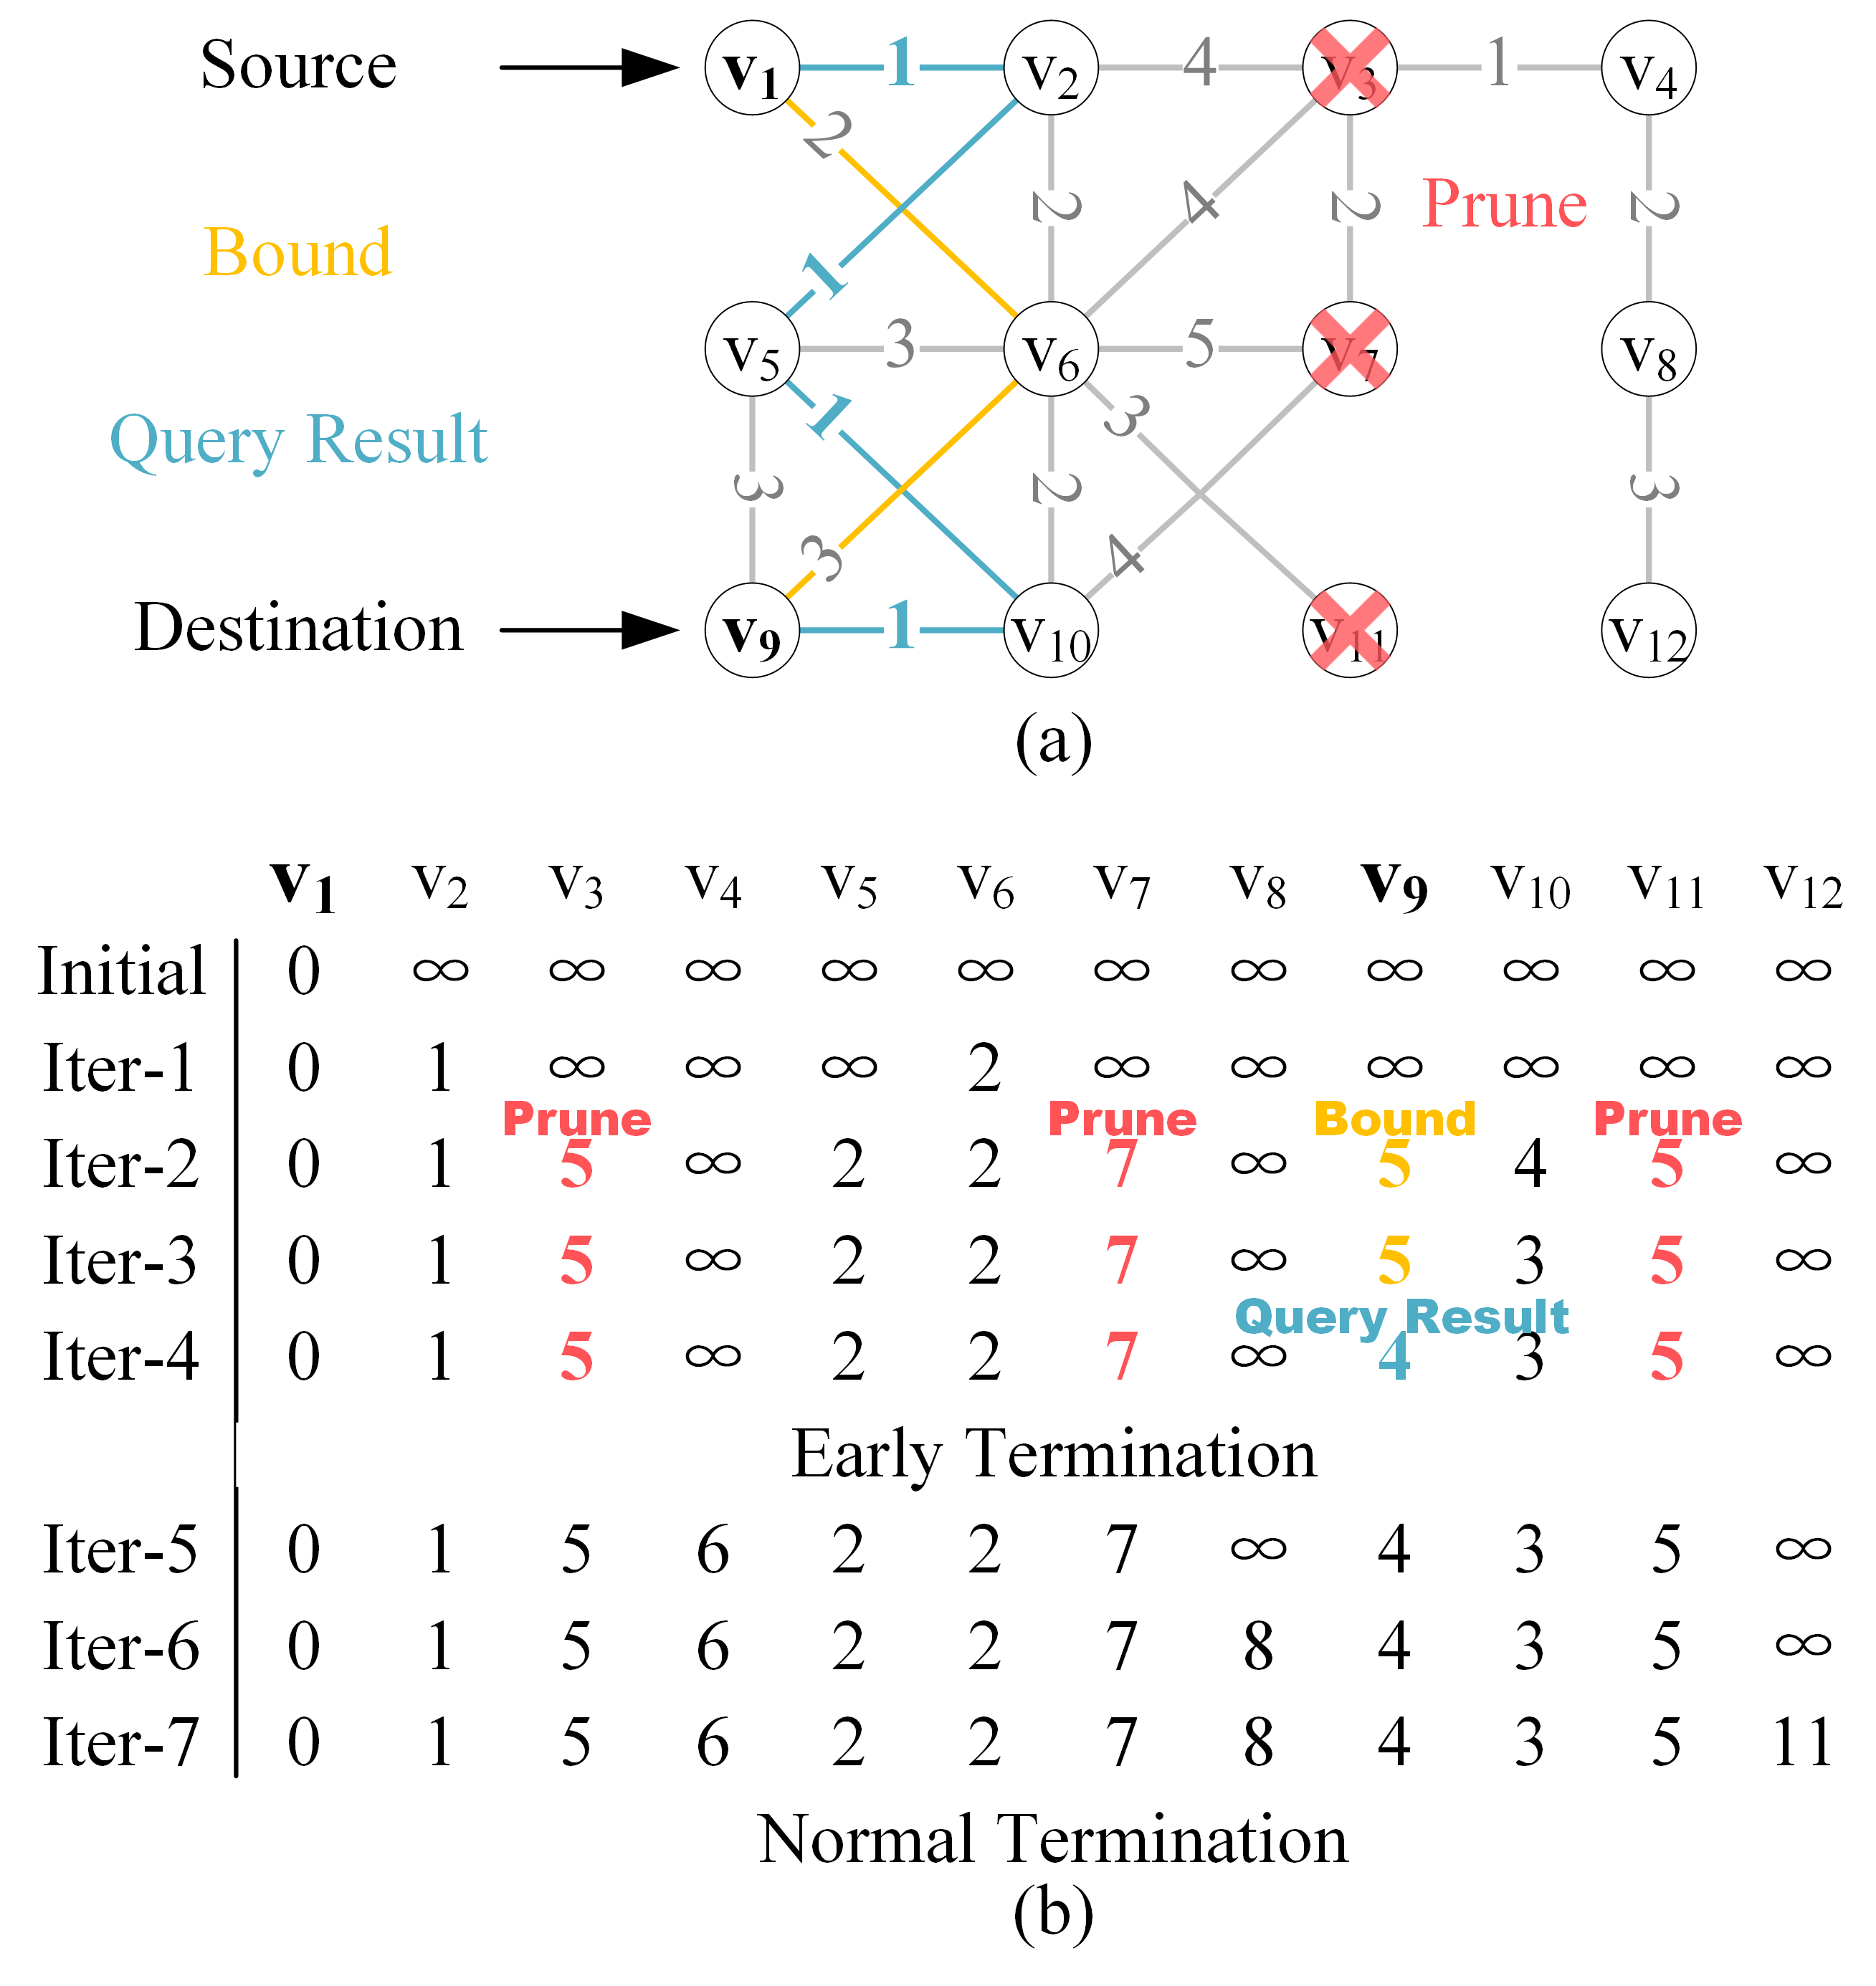
\includegraphics[width=\columnwidth]{picture/Zhang-fig1.png}
    \captionsetup{labelsep=period}
    \caption{\centering{The scheduling processes of task-driven and data-driven}}
    \label{fig1}
    \vspace{-0.5cm}
\end{figure}

Queries on the underlying graph exhibit an overlap effect, where the traversal paths formed by these tasks intersect. Our experiments reveal that 72\%-90\% of vertices in a graph are accessed by multiple queries (Figure \ref{fig3}), leading to significant {\bf{redundant data access}}.
Additionally, natural graphs follow a power-law distribution, with a small number of vertices connecting to numerous edges. These vertices are frequently involved in the computation processes of different queries, constituting 75\%-95\% of the total computation (Figure \ref{fig4}). The repeated process for these highly connected vertices caused by different queries results in {\bf{redundant computation}}.
However, as illustrated in Figure \ref{fig1}, existing query systems adopt a task-driven approach, independently accessing and processing the necessary data without inter-query cooperation, which fails to effectively address redundant overhead. Moreover, with an increase in concurrency, the situation even exacerbates.

Some solutions, such as Glign \cite{glign}, attempt to optimize the throughput of general concurrent graph processing. However, Glign primarily focuses on point-to-all algorithms and lacks an appropriate mechanism to fully leverage the unique characteristics of point-to-point queries, thus failing to avoid redundant path traversals.
Additionally, another solution SGraph \cite{sgraph}, proposes a computation sharing approach. It selects high-degree vertices and performs point-to-all queries with these vertices as the starting or ending vertices, storing the query results during the preprocessing phase.
In this way, tasks requiring the execution of queries associated with these high-degree vertices can benefit from avoiding recomputation.
This approach reduces the query response time by pre-computing and sharing the results that may be queried. 
However, it introduces a substantial overhead, as its computational and storage requirements typically scale proportionally with the size of the graph, making them unaffordable for large graphs.

Driven by the increasing demand for concurrent point-to-point queries and recognizing the limitations of current solutions, we present GraphCPP—a novel data-driven system designed to optimize concurrent query throughput.
GraphCPP integrates a data access sharing mechanism to facilitate concurrent queries with shared data access. It divides the data needed by query into task-specific information, which remains private to each query thread, and graph structure data, which is uniformly managed through a data-sharing mechanism. Subsequently, utilizing a priority scheduling strategy, the system loads graph blocks into the Last Level Cache (LLC). Following this, an association mechanism triggers the execution of queries related to the loaded block. These queries share the same graph structure data in LLC, eliminating redundant data access and amortizing data access overhead.
Additionally, drawing inspiration from logistics networks that optimize efficiency through hub stations and high-speed connections, GraphCPP employs a dual-level computation sharing mechanism to optimize query speed. This mechanism consists of two components: the Global Vertices and Core Subgraph Mechanisms. They identify frequently accessed vertices and paths, precomputing or dynamically obtaining their query results during runtime. Such pre-calculated information can be efficiently reused by subsequent queries, significantly boosting processing speed.


This paper makes the following contributions:
\begin{enumerate}
  \item{{\bf{Analysis of Performance Bottlenecks}}: we analyze the performance bottlenecks of existing systems for concurrent point-to-point queries and identify potential optimization opportunities through data access and computation sharing.}
  \item{{\bf{GraphCPP Design}}: we introduce GraphCPP, a novel data-driven graph processing system specifically designed for concurrent point-to-point queries. GraphCPP leverages redundancies in data access and computation across concurrent queries to achieve significant performance improvements.}
  \item{{\bf{Evaluation and Performance}}: we conduct comprehensive evaluations comparing GraphCPP against state-of-the-art systems on a diverse workload using real-world graphs and applications. The results demonstrate that GraphCPP surpasses SGraph by an average of 3.2×.}
\end{enumerate}

The remaining content is structured as follows: Section \ref{motivation} provides background information and outlines our motivation. Section \ref{overview} details the implementation specifics of GraphCPP, followed by the experimental evaluation in Section \ref{experimental}. Section \ref{relate_work} reviews related work, and lastly, we present our conclusions in Section \ref{conclusion}.


\vspace{-8pt}
\section{Background and Motivation}\label{motivation}
%This section first introduces the out-of-core concurrent graph processing systems, and then explains our observations on the I/O inefficiency when existing systems handle concurrent graph processing jobs.


\vspace{-4pt}
\subsection{Point-to-Point Query}\label{2.1}
\vspace{-4pt}
{\bf{Application.}} The point-to-point query is utilized to retrieve specific {\bf{query results}} between particular vertex pairs in a graph. It is typically divided into two categories: 1) Weighted graph algorithms: Point-to-point shortest path (PPSP) \cite{ppsp}, point-to-point widest path (PPWP) \cite{ppwp}, and point-to-point narrowest path (PPNP) \cite{ppnp} are employed to identify the shortest, widest, or narrowest path between two vertices, respectively. They find extensive applications in social/financial networks, traffic planning, monitoring money laundering activities, and network quality analysis. 2) Unweighted graph algorithms: Breadth-first search (BFS) \cite{bfs}, connectivity \cite{connectivity}, and reachability \cite{reachability} are used to determine layering (BFS) or reachability of specific vertex pairs in undirected (connectivity) or directed graphs (reachability). These algorithms are widely applied in bi-connectivity, higher-order connectivity, and advanced algorithms for graph clustering.

{\bf{Procedure.}} In Figure \ref{fig2}, we illustrate the steps of the point-to-point algorithm by employing the PPSP algorithm on an undirected graph.
Figure \ref{fig2}(a) illustrates the structural details of the graph, with $v_1$ serving as the source vertex and $v_9$ serving as the destination vertex. The corresponding edge weights are denoted as $W_{(v_1,v_9)}$. The query is represented as $Q(v_1\rightarrow v_9)$.
In Figure \ref{fig2}(b), specific details related to the query are tracked, including active vertices ($v_i$) and their corresponding query results ($R(v_1,v_i)$) from $v_1$ to $v_i$ in each iteration. The query result signifies the shortest distance between the corresponding vertices, with its value dynamically updated during the iterations, and its interpretation varies with specific algorithms. Specifically, the best-known query result in the current iteration from the source vertex to the destination vertex ($R(v_1,v_9)$) is referred to as the {\bf{bound}}.
Initially, $v_1$ is the only active vertex, setting $R(v_1,v_1)$ to 0, and the query results for other vertices are initialized to infinity since they are unknown. Subsequent iterations involve traversing outgoing neighbors ($v_j$) of active vertices ($v_i$). If $R(v_1,v_i) + W_{(v_i,v_j)} < R(v_1,v_j) < {bound}$ or $R(v_1,v_i) + W_{(v_i,v_j)} < R(v_1,v_j) = {bound} = \infty$, then $R(v_1,v_j)$ is updated to the value of $R(v_1,v_i) + W_{(v_i,v_j)}$, and $v_j$ becomes the active vertex in the next iteration. Otherwise, the corresponding path is pruned.
In the first iteration, we traverse the outgoing neighbors ($v_2$ and $v_6$) of the starting point ($v_1$) and obtain their query results from the starting point ($R(v_1,v_2)$ and $R(v_1,v_6)$), which are equal to the weights of their edges with the starting point. The activated $v_2$ and $v_6$ are added to the set of active vertices ($V_{active}$) for the next iteration.
In the second iteration, the algorithm identifies a valid path from the source to the destination vertex: $v_1\rightarrow v_6\rightarrow v_9$. The query result of this path ($R(v_1,v_9)$) is used as the bound. All paths with query results worse than the bound are terminated early, leading to the pruning of paths to $v_3$, $v_7$, and $v_{11}$. As iterations progress, the bound value is continuously updated.
In the fourth iteration, a better query path is discovered: $v_1\rightarrow v_2\rightarrow v_5\rightarrow v_{10}\rightarrow v_9$, and the bound is updated with $R(v_1,v_9)$. At this point, all outgoing edges of active vertices have been pruned, resulting in no active vertices in the next iteration. Consequently, the query terminates early, and the bound value at this point becomes the final query result. The described pruning steps effectively reduce redundant data access and computations in point-to-point queries.

\begin{figure}[t]
    \centering
    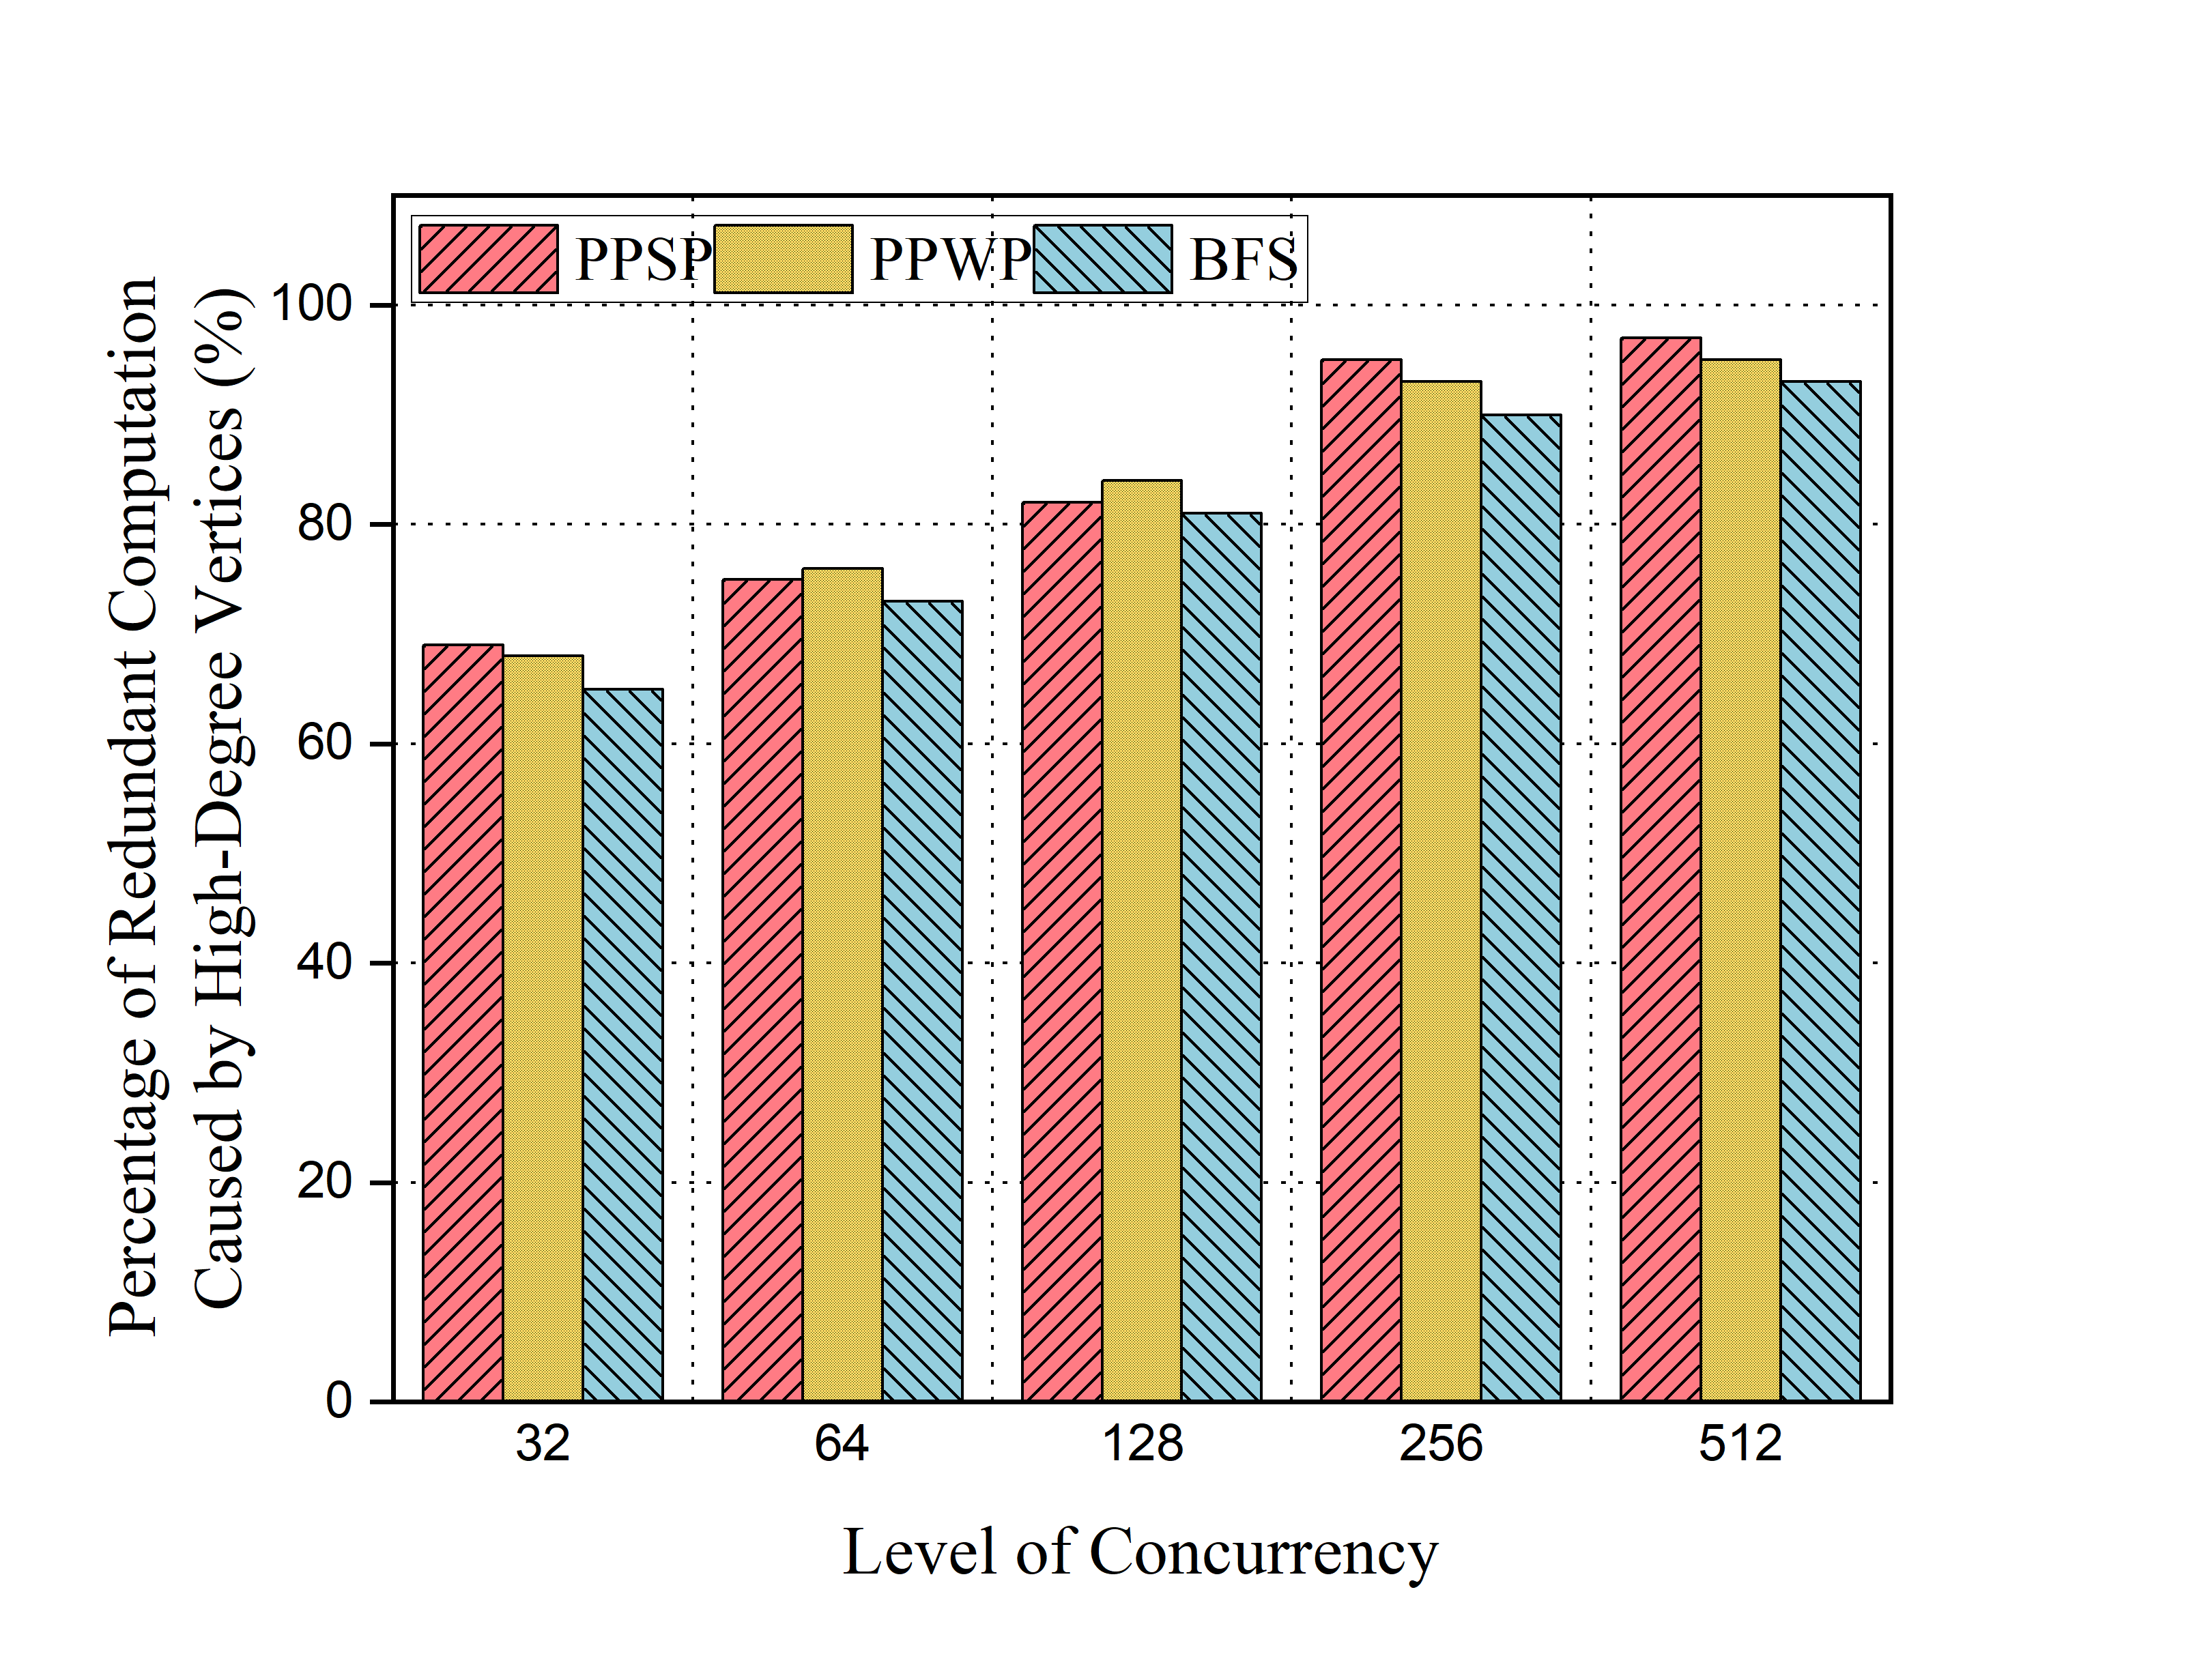
\includegraphics[width=\columnwidth]{picture/Zhang-fig2.png}
    \captionsetup{labelsep=period}
    \caption{\centering{Point-to-point shortest path query $Q(v_1\rightarrow v_9)$}}
    \label{fig2}
    \vspace{-0.5cm}
\end{figure}
{\bf{Pruning~Mechanism.}}
The primary optimization for these algorithms lies in the pruning mechanism \cite{sgraph}, which eliminates unnecessary path traversals, allowing iterative queries to converge more quickly. 
Taking PPSP as an example, this process can be summarized in three stages: 1) Establishing a valid query result as the initial bound; 2) Evaluate paths based on specific criteria. If a path's query result is better than the current bound, update the bound and continue exploration. Otherwise, prune the path to avoid further unnecessary computation; 3) The process continues until no paths' query results are better than the current bound. This signifies reaching the optimal solution, with the bound representing the final converged result.
 three-stage pruning processes exist for other point-to-point queries, though the specific details and comparison rules vary. Table \ref{table1} illustrates the diverse meanings of bounds and their corresponding comparison rules across different algorithms.



For the PPSP algorithm, the bound represents the distance value of the shortest path from vertex $v_i$ to $v_j$ in each iteration. The algorithm's rule compares the distance of different paths. Any paths with distances greater than the bound are pruned.
In the case of the PPWP/PPNP algorithm, the bound signifies the maximum (minimum) edge weight among all reachable paths from the source vertex ($v_s$) to the destination vertex ($v_d$) during an iteration. The rule dictates that if any edge weight in the path is narrower (wider) than the current bound, the corresponding path is pruned.
For the point-to-point version of the BFS algorithm, the bound denotes the minimum layer count from vertex $v_s$ to $v_d$.
In connectivity or reachability algorithms, the bound indicates the connectivity from vertex $v_s$ to $v_d$ in undirected and directed graphs, respectively.
The three algorithms mentioned later have a unique characteristic: once they encounter any valid path, it signifies the discovery of the desired optimal path, and the query concludes at that point. For instance, during the first traversal, BFS determines the shortest path to the endpoint. Once the path's accessibility is confirmed for the first time, there is no need to search for other reachable paths.

\begin{table}[t]
    \centering
    \renewcommand\arraystretch{1.2}
    \scriptsize
    \begin{tabular}{c c c}
    \hline
    \rule{0pt}{8pt} 
    Algorithm           & Meaing of Bound         &Criterion for Comparison\\
    \hline
    \rule{0pt}{8pt}
    PPSP                & shortest distance         & disatance     \\
    PPWP                & weight of widest edge             & weight     \\
    PPNP                & weight of narrowest edge             &weight      \\
    BFS                 & shortest layer              & number of layers      \\
    Reachability        & undirected graph connectivity       & reachability      \\
    Connectivity        & directed graph connectivity         & reachability     \\
    \hline
    \end{tabular}
    \caption{\centering{Details of different point to point query algorithms}}
    \label{table1}
\end{table}
\vspace{-0.5cm}
\subsection{Performance Bottlenecks in Concurrent Point-to-Point Queries}\label{2.2}
While extensive researches have been conducted on optimizing single point-to-point queries, effectively handling concurrent queries remains a challenge. 
To systematically evaluate the performance challenges of concurrent point-to-point queries, we examine the LLC miss ratio and redundant computation ratio of different systems as the concurrency level varies within a batch. In this context, we consider the computation of path segments that overlap among different queries as a redundancy. We implemented the concurrent version of point-to-point query systems: PnP and SGraph, and extended the general concurrent processing system Glign with pruning capabilities to support point-to-point queries. Experiments were conducted using a total of 512 queries with varying concurrency levels on the TW dataset. 
Table \ref{table2} illustrates an increase in LLC miss rates as the concurrency level rises. Notably, Glign demonstrates robust support for concurrent tasks, achieving the lowest miss ratio under  conditions.
Additionally, our analysis of traversal results within query batches reveals a positive correlation between concurrency and the occurrence of redundant computation in all systems. This correlation arises because, as the number of concurrent queries increases, the proportion of path segments that are computed more than once also increases.
Glign exhibits a higher redundancy computation ratio than other solutions due to its lack of point-to-point query optimizations. As a result, many paths that should be pruned are computed.
In a task-driven execution module, threads operate independently, leading to increased contention for shared resources. This results in redundant data access and computation overhead, which causes performance bottlenecks for concurrent point-to-point queries.

\begin{table}[h]
 	\centering
 	\renewcommand\arraystretch{1.2}
 	\scriptsize
 	\begin{tabular}{c c c c c c}
 		\hline
 		\rule{0pt}{13pt} 
 		\multirow{1}{*}{} & {\makecell[c]{Number of \\ concurrent queries}} & {PnP} & {SGraph} & {Glign} \\
 		\hline
 		\rule{0pt}{8pt}   
 		\multirow{4}{*}{\makecell[c]{LLC miss \\ ratio}}
 		& 1 & 41.1\% & 35.9\%  & 28.4\% \\
 		& 32 & 59.4\% & 54.0\% & 32.2\% \\
 		& 64 & 71.4\% & 67.2\% & 38.5\% \\
 		& 128 & 80.3\% & 76.7\% & 43.4\% \\
 		& 512 & 89.6\% & 84.7\% & 49.4\% \\    
 		\hline
 		\rule{0pt}{8pt}   
 		\multirow{4}{*}{\makecell[c]{Redundant \\ computation ratio}}
 		& 1 & - & - & - \\
 		& 32 & 65.6\% & 51.9\% & 72.9\% \\
            & 64 & 74.4\% & 64.9\% & 84.8\% \\
            & 128 & 85.6\% & 72.1\% & 92.6\% \\
            & 512 & 96.8\% & 80.4\% & 97.4\% \\
 		\hline
 	\end{tabular}
 	\caption{\centering{Performance analysis of systems with varying concurrency (512 PPSP queries on TW \cite{twitter})}}
 	\label{table2}
        \vspace{-0.5cm}
\end{table}



\subsection{Our Motivation}\label{2.3}
The mentioned challenges hinder the effectiveness of current solutions for handling concurrent point-to-point queries, yet they also create an opportunity through the sharing of data access and computation.
In real-world graphs, a small fraction of vertices is connected to the majority of edges, resulting in a characteristic power-law distribution.
\textit{We refer to these heavily interconnected vertices as \textbf{\textit{hot~vertices}} and term the convergent path obtained from executing point-to-point queries for pairs of hot vertices as \textbf{\textit{hot~paths}}.}
Through a thorough analysis of the concurrent query process, we observe that hot vertices and hot paths account for the majority of redundant overhead.
Using the PPSP example in Figure 2, queries $Q(v_1\rightarrow v_{9})$, $Q(v_1\rightarrow v_{10})$, and $Q(v_2\rightarrow v_{9})$ independently recomputed the path from $v_2$ to $v_{10}$, incurring redundant overhead. For these queries, $v_2$, $v_5$, and $v_{10}$ are identified as hot vertices, and the path $v_2\rightarrow v_5\rightarrow v_{10}$ is termed a hot path.
Therefore, by identifying hot vertices and sharing information about hot paths, we can significantly reduce redundant computations and enhance the efficiency of concurrent point-to-point queries. Further details are provided below.

{\bf{Data Access Sharing.}}
Queries originating from different points often access the same vertices during traversal.
In Figure \ref{fig3}, we record the traversal paths of concurrent queries within the same batch and analyze the proportion of vertices accessed more than once by different queries to the total activated vertices. When the query concurrency in a batch reaches 512, over 90\% of the vertices are accessed more than once. However, in the existing task-driven execution module, different queries independently access their required data, resulting in redundant access to the same data. 
\textit{Enabling queries to share access to the same graph structure data can amortize the data access overhead, significantly improving the overall throughput of concurrent query processing.}


{\bf{Computation Sharing.}}
As depicted in Figure \ref{fig1}, various queries frequently recompute the results of identical hot path segments during traversal, resulting in redundant computations.
In Figure \ref{fig4}, we identify the intersection of various query paths, redundantly processed by all queries in a batch. We then select the top 522 hot vertices, constituting less than 1\% of the total, and analyze their proportion in query intersections under different concurrency levels. As concurrency increases, the total amount of overlapping data decreases, while the percentage of hot vertices in this overlap can increase to 95\% (at 512 concurrency). This indicates that hot vertices and their corresponding hot paths significantly impact redundant computations.
\textit{Facilitating the sharing of computations for hot paths among distinct queries can significantly mitigate computational overhead and enhance query efficiency.}
\begin{figure}[t]
	\centering
	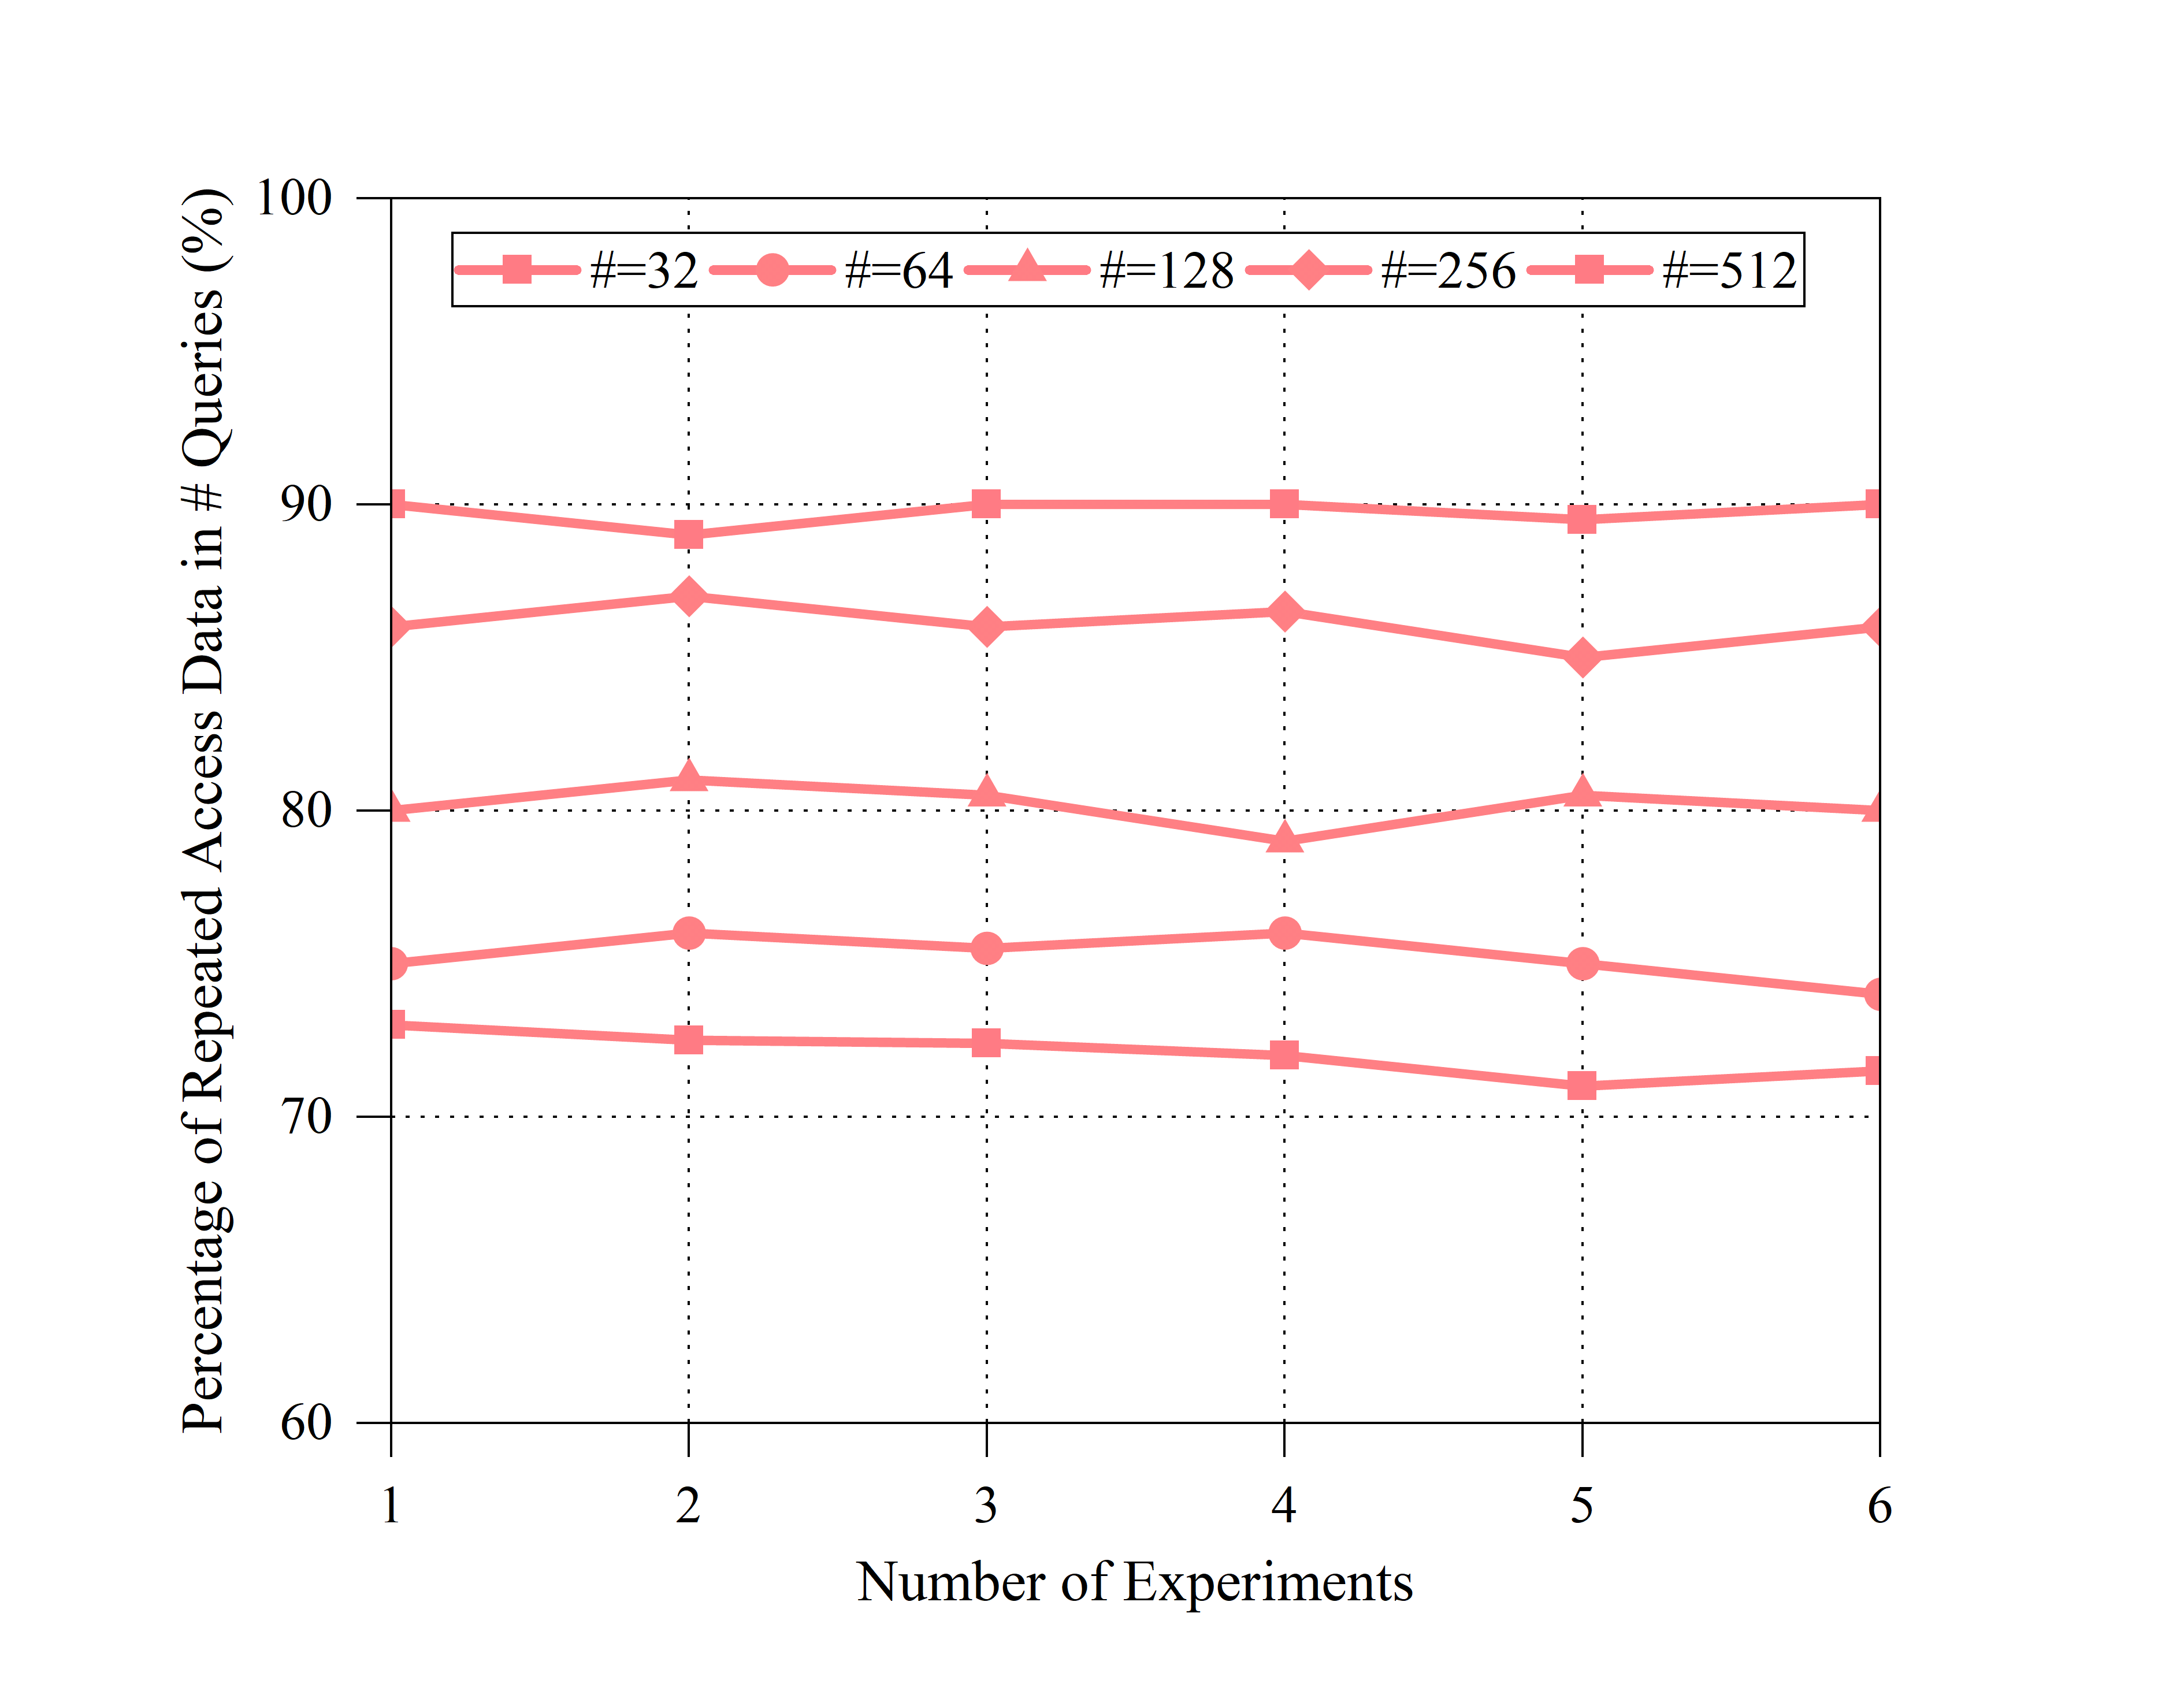
\includegraphics[width=3.0in]{picture/Zhang-fig3.png} %调节单个子图大小
	%\setlength{\abovecaptionskip}{-0.05cm} %控制标题与子图距离
    \captionsetup{labelsep=period}
		\caption{\centering{Data access redundancy among concurrent queries}} %子图下标题
		\label{fig3} %引用标签            
\end{figure}

\begin{figure}[t]
	\centering
	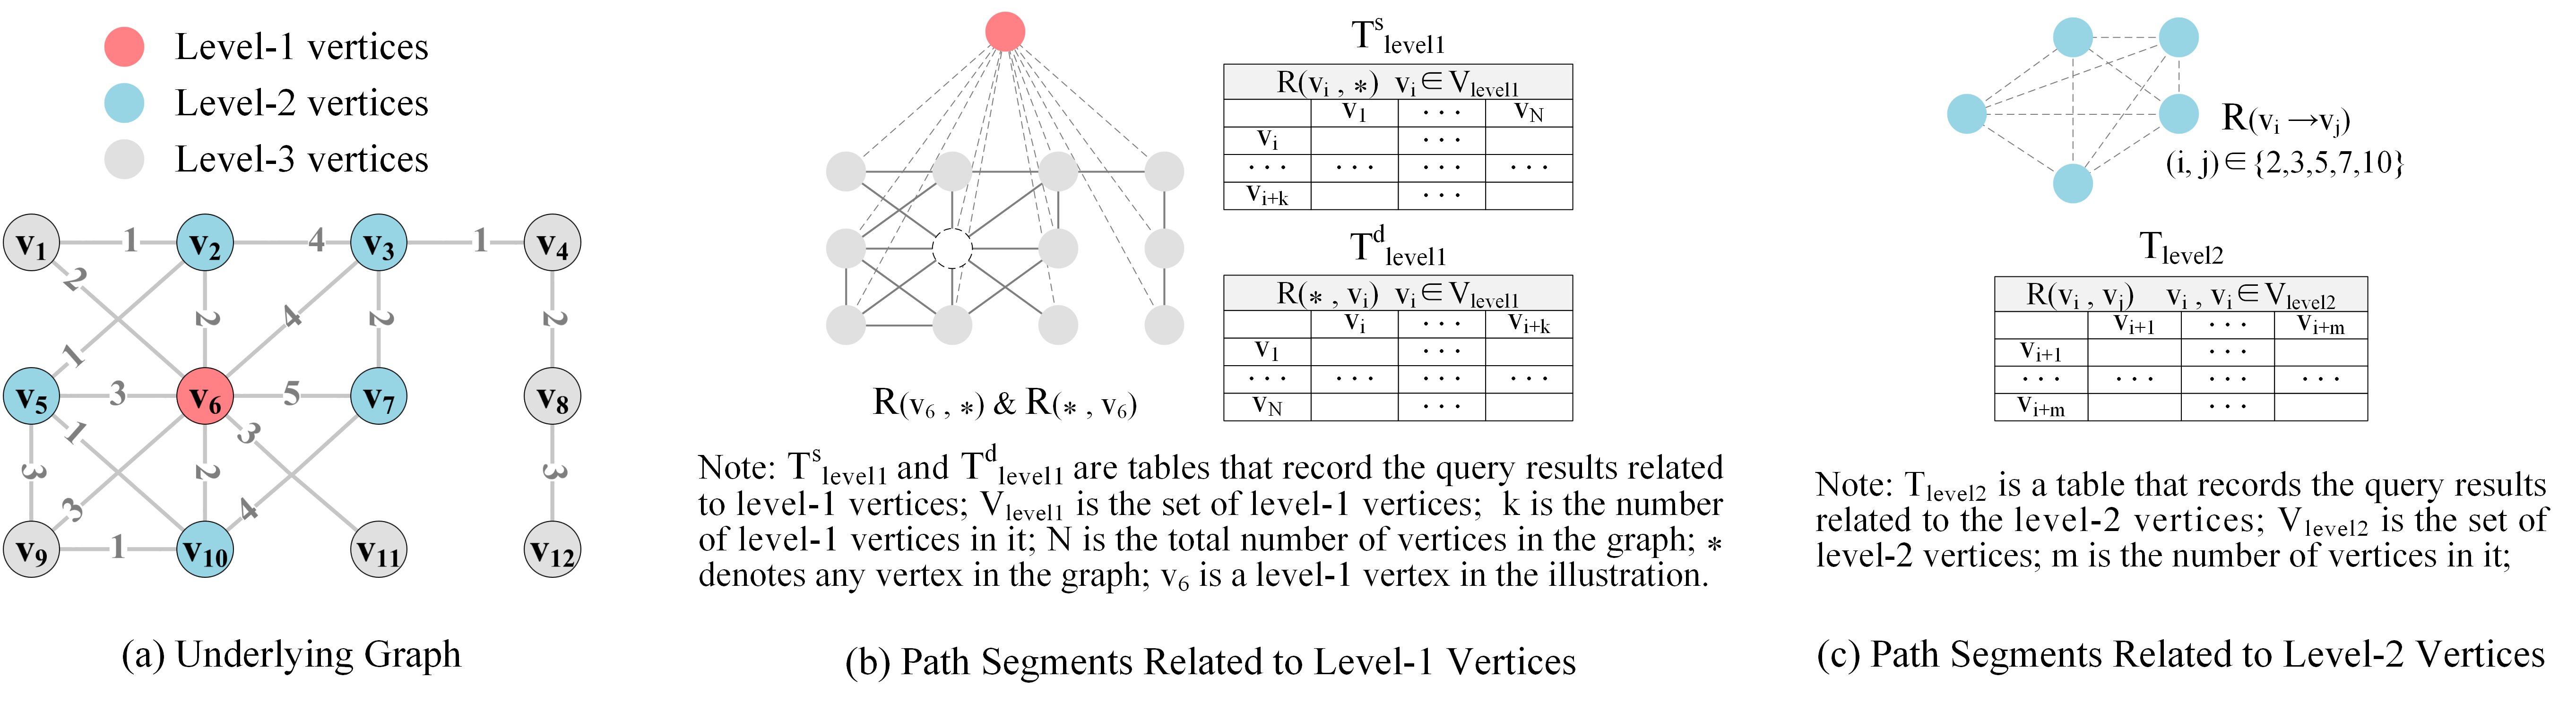
\includegraphics[width=3.0in]{picture/Zhang-fig4.png}
	%\setlength{\abovecaptionskip}{-0.05cm} 
    \captionsetup{labelsep=period}
		\caption{\centering{Computation redundancy among concurrent queries}}
		\label{fig4}
            \vspace{-0.5cm}
\end{figure}


\vspace{-6pt}
\section{Overview Of GraphCPP}\label{overview}
\begin{figure}[t]
    \centering
    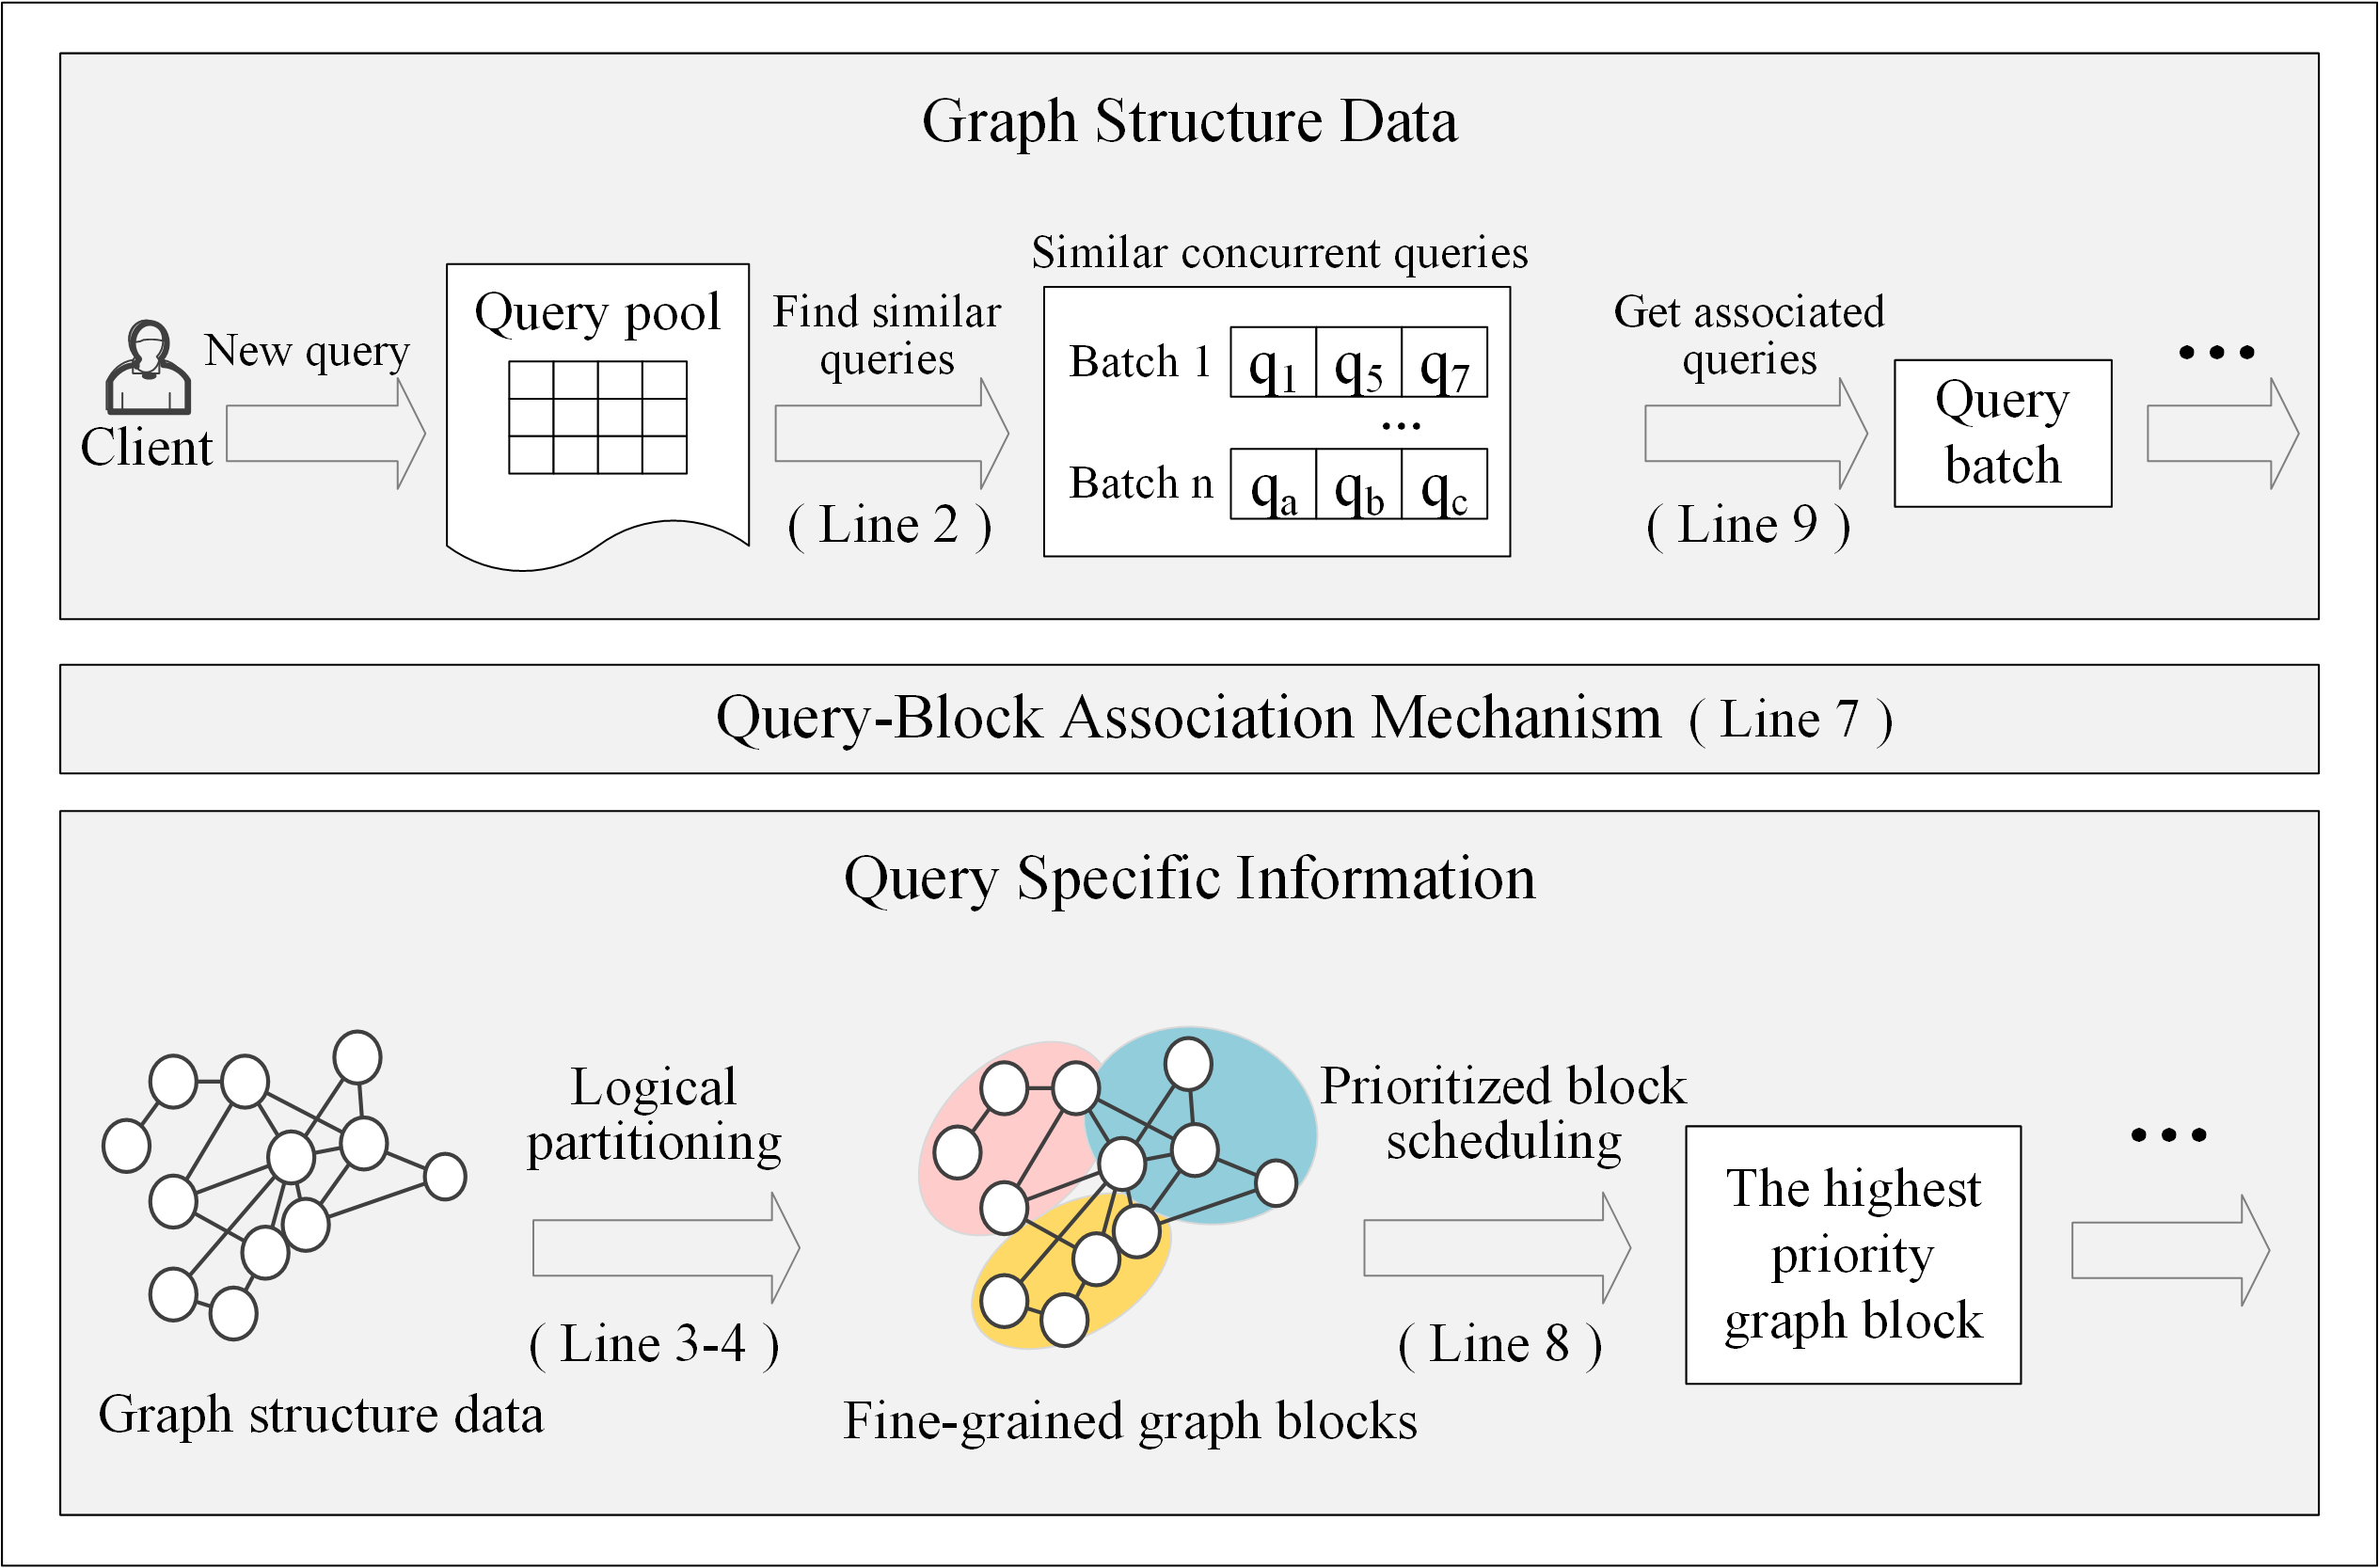
\includegraphics[width=\columnwidth]{picture/Zhang-fig5.png}
    %\setlength{\abovecaptionskip}{-0.05cm} 
    \captionsetup{labelsep=period}
    \caption{\centering{System architecture diagram}}
    \label{fig5}
    \vspace{-0.5cm}
\end{figure}
To enhance the efficiency of concurrent point-to-point queries, we introduce GraphCPP, a system designed to leverage data access and computation sharing among concurrent queries. It incorporates a novel data-driven caching execution mechanism to amortize data access overhead among multiple tasks. Additionally, it introduces a dual-level computation sharing mechanism, enabling computations for hot vertices and hot paths to be shared across queries.
In this section, we will present an overview of GraphCPP. Section \ref{3.1} introduces the overall architecture. Section \ref{3.2} describes the data access sharing mechanism, and Section \ref{3.3} describes the computation sharing mechanism.

\subsection{System Architecture}\label{3.1}
GraphCPP adopts a four-layer architecture, as depicted in Figure \ref{fig5}. 
The {\bf{storage layer}} stores the graph structure data and the query specific information. 
In the {\bf{preprocessing layer}}, graph structure information in memory is logically divided into fine-grained graph blocks, which can be suitably accommodated within LLC. Additionally, a query similarity-aware mechanism is implemented to cluster queries from the query pool into groups based on their similarities, thereby enhancing data access sharing efficiency by concurrently executing  queries in a batch.
The {\bf{scheduling layer}} conducts scheduling based on the associations between blocks and queries. In this context, the term `association' indicates that a specific graph block contains active vertices required by a particular query. This layer will establish associations between blocks and queries, as well as quantify the number of tasks associated with each graph block. It consists of two main components:
1) Priority Block Scheduling: Blocks with a higher number of associated tasks are prioritized for scheduling because they benefit more from sharing.
2) Associated Task Trigger: Once the scheduling layer identifies blocks for shared execution, it proceeds to determine all queries associated with these blocks.
These associated queries form a subset of the  query set.
Simultaneously processing these associated tasks on shared graph blocks enables multiple queries to leverage the same underlying graph structure data, effectively reducing the data access overhead.
The {\bf{engine layer}} is the core of GraphCPP, and it consists of two components:
1) Data Access Sharing Mechanism: This mechanism identifies shared graph structure data accessed by multiple tasks, and employs a data-driven scheduling approach to enable concurrent queries to share the same data.
2) Dual-level Computation Sharing Mechanism: This mechanism exploits the fact that different queries often compute the results for the same hot paths. By facilitating the pre-computing and sharing of these computations across different queries, this mechanism optimizes query processing and effectively reduces computation redundancy.

\begin{figure}[t]
	\centering
	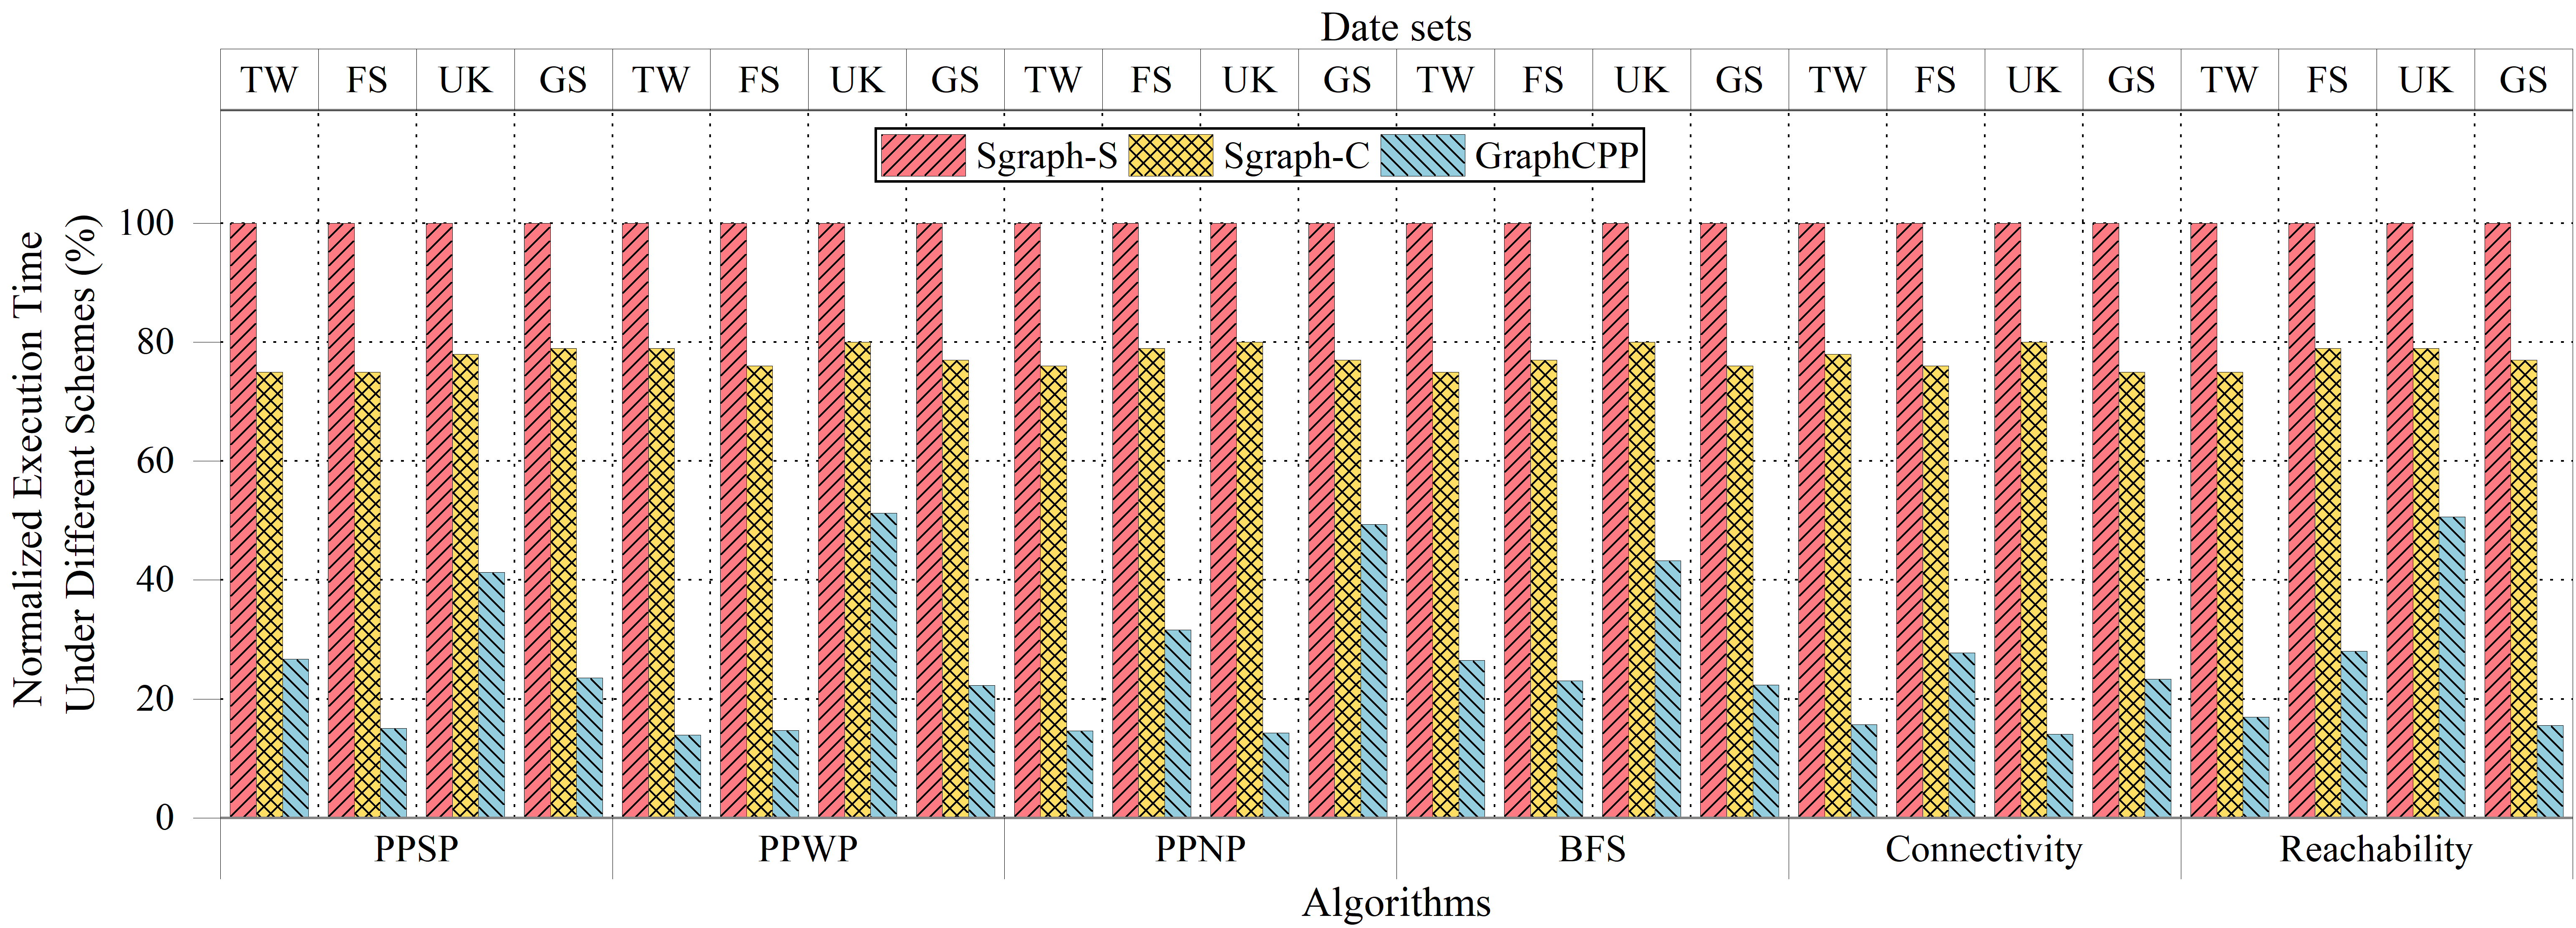
\includegraphics[width=\columnwidth]{picture/Zhang-fig6.png} %调节单个子图大小
	%\setlength{\abovecaptionskip}{-0.05cm} %控制标题与子图距离
    \captionsetup{labelsep=period}
		\caption{\centering{Data Access Sharing Mechanism}} %子图下标题
		\label{fig6} %引用标签
\end{figure}%


\begin{algorithm}[t]
\caption{Data Access Sharing Algorithm}
\label{alg:data_access_sharing}
\begin{algorithmic}[1]
\Function{DataAccessSharing}{$Q$, $G$}
	\State $Q_{similar} \gets$ FindQueries($Q$)
	\State $S_{block} \gets$ DetermineSharedBlockSize()
	\State $T_{block} \gets$ LogicalPartition($G$, $S_{block}$)
	\State $V_{active} \gets$ InitializeActiveVertexSet($Q_{similar}$)
	\While{$V_{active}$ is not empty}
		\State UpdateAssociationInfo($V_{active}$, $T_{block}$)
		\State $b_i \gets$ BlockPrioritizeSchedule()
		\State $Q_{b_i} \gets$ GetAssociatedQueries($b_i$)
		\State $V_{active} \gets$ ComputationSharing($b_i$, $Q_{b_i}$)
	\EndWhile
	\State \textbf{return} $R$
\EndFunction
\end{algorithmic}
\end{algorithm}

\vspace{-8pt}
\subsection{Data Access Sharing Mechanism}\label{3.2}
In Section \ref{motivation}, we observed a significant overlap in graph structure data accessed by concurrent queries. However, under the current processing approach, this overlap data cannot be utilized effectively. For monotonic point-to-point queries on the graph, the order of data access does not affect the accuracy of the final results. Thus the core idea of our data sharing mechanism is to transform the conservative sequential, coarse-grained task-driven scheduling order into a concurrent, fine-grained data-driven approach. This approach addresses data redundancy among concurrent queries to amortize data access overhead, improve cache utilization efficiency, and consequently, enhance system throughput. The pseudo-code in Algorithm 1 illustrates the implementation of the Data Sharing Mechanism, which is consistent with the step in Figure \ref{fig6}.

The function, named \texttt{DataAccessSharing}, accepts two parameters: $Q$ and $G$, representing all requests in the query pool and the graph structure data, respectively (line 1). The algorithm commences by identifying  query set within the query pool, denoted as $Q_{similar}$ (line 2). Subsequently, the size of shared data blocks ($S_{block}$) is determined (line 3). We then employ a logical partitioning approach to subdivide coarse-grained graph partitions into fine-grained blocks ($S_{block}$). The information of logical partitioning is stored in $T_{block}$, a dictionary data structure that records the mapping relationship between physical data and logical partitions (line 4). Following this, the active vertex set ($V_{active}$) is initialized based on the $Q_{similar}$ (line 5). The algorithm iterates until $V_{active}$ is empty (line 6). In each iteration, the association information between active vertices and graph blocks is updated (line 7). The algorithm prioritizes the selection of graph blocks using the \texttt{BlockPrioritizeSchedule} function (line 8). Then, it retrieves the associated tasks using the \texttt{GetAssociatedQueris} function (line 9). Next, computation sharing is performed on the selected block and query set (line 10). This updates $V_{active}$ for the next iteration. When all active vertices have been processed, indicating that the query batch has been completed, the algorithm returns the computation results (line 12).
This part provides an overview of the algorithm's flow, with further details to be explored in the following parts.

{\bf{Find Similar Queries.}} The query pool often contains numerous queries that exceed the concurrent limit. Hence, it's necessary to group these queries for batch processing. Queries within the same batch run concurrently, while those in different batches are processed sequentially. The degree of overlap among query paths can vary significantly, with some sharing many common path segments and others having minimal overlap. Therefore, the selection of query tasks within a batch can significantly impact overall system performance.
To address this, we employ an intuitive similarity-aware approach for grouping queries within a batch. It calculates the similarity between queries $q_i$ and $q_j$ using the following formula, where $v_{src}^i$ and $v_{dst}^i$ denote the source and destination vertices of query $q_i$ respectively, and $D(v_i,v_j)$ represents the distance between two vertices ($v_i$ and $v_j$) using PPSP. The corresponding value increases as the similarity between queries rises. Specifically, we randomly select a query $q_i$ and compute its similarity with other queries. If the similarity between a task and $q_i$ exceeds a predefined threshold (we set it to 0.1 in our experiments), it's considered a similar query to $q_i$. Once enough similar queries fill a batch, they are executed concurrently.
Since similarity computation can be performed in the background while executing query tasks, the overall overhead is minimal.

\begin{equation}
{Similarity} = \frac{1}{{D}(v_{src}^i,v_{src}^j) + {D}(v_{dst}^i,v_{dst}^j)}
\end{equation}


{\bf{Determine shared block size.}} Cache plays a critical role in hierarchical storage systems. Therefore, it is important to select an appropriate shared graph block size to maximize cache utilization. Ideally, the shared graph block size should be small enough to fit into the LLC, yet not so small as to cause excessive scheduling overhead during query processing. Formula 2 is employed to calculate the maximum size for shared graph blocks, taking into account factors including shared block size ($S_{block}$), partition size ($S_{graph}$), total number of vertices ($|V|$), average storage cost per vertex ($S_{vertex}$), number of concurrent queries ($N$), LLC size ($S_{LLC}$), and reserved redundant space ($S_{reserve}$) determined by empirical judgment. By considering both graph structure and query-specific information, this formula enables us to determine the maximum granularity for each shared graph block while ensuring efficient utilization of the available LLC capacity.
\begin{equation}
    S_{block} + \frac{S_{block}}{S_{graph}} \cdot \lvert V \rvert \cdot S_{vertex} \cdot N \leq S_{LLC} - S_{reserve}
    \end{equation}

{\bf{Logical partitioning.}} After determining the shared block size, we apply this granularity to perform logical graph partitioning. Given that each edge in the graph structure dataset occupies a fixed size, we can calculate the maximum number of edges a shared block can accommodate. Subsequently, we partition the edges in the edgelist based on this calculated value. Since the edgelist is arranged in ascending order by source vertex ID, it suffices to record the start and end vertex IDs for each block. Due to variations in the out-degree of each vertex, resulting in a uniform division may amortize a vertex's different out-edges across multiple blocks. Therefore, we additionally store the count of edges associated with a specific vertex in a given block. This approach allows us to partition the physically contiguous graph structure data into logically independent blocks. The partitioning information is stored in $T_{block}$, and during data access, we can determine the physical location of a block by referring to the vertex ID and edge count saved in $T_{block}$.


{\bf{Update the association information between blocks and queries.}} In our data-driven scheduling model, it is essential to update the association between blocks and queries in each iteration. The dynamic relationship between a graph block and a query is determined by the query's active vertex set ($V_{active}$).
If a graph block contains active vertices required by a query, then the block is associated with the query. By tracking each query's traversal process during an iteration, we can predict $V_{active}$ for the next round. Leveraging the $T_{block}$, we efficiently map these active vertices to their corresponding graph blocks, updating the graph block-query association. Although this association dynamically updates with each execution, the low number of active vertices ensures minimal overhead for maintaining these connections.


{\bf{Block prioritize schedule}}. Following the established associative relationship between blocks and queries, we implement prioritized scheduling for graph blocks to address data access redundancy among concurrent queries. This approach prioritizes blocks with the greatest potential for shared data utilization across tasks, ultimately enhancing system performance. The calculation of priority follows the formula below.

\begin{equation}
{Priority} = w_1 \cdot {N}_{{query}} + w_2 \cdot \left(\frac{{N}_{{hot}}}{{N}_{{active}}}\right)
\end{equation}


Here, ${N}_{{query}}$ denotes the number of queries associated with the block, and $\frac{{N}_{{hot}}}{{N}_{{active}}}$ represents the proportion of active hot vertices within a block out of the total active vertices. $w_1$ and $w_2$ are weight parameters that balance the influence of these factors, with their values manually tuned. 
In our experiments, $w_1$ is set to 0.5, and $w_2$ is set to 1.
The computed priority determines the sequence for loading graph blocks into the LLC, giving preference to those with higher priority and thus facilitating efficient data sharing.

\vspace{-6pt}
\subsection{Computation Sharing Mechanism}\label{3.3}
Recognizing that most of this redundancy is attributed to hot vertices and hot paths in Section \ref{2.3}, we introduce a dual-level computation sharing mechanism to share their query results among different queries. Query results represent the converged outcomes of executing the respective point-to-point query algorithm for a specific vertex pair.
The operational process of this mechanism is illustrated in Figure \ref{fig7}:

\begin{figure*}[t]
    \centering
    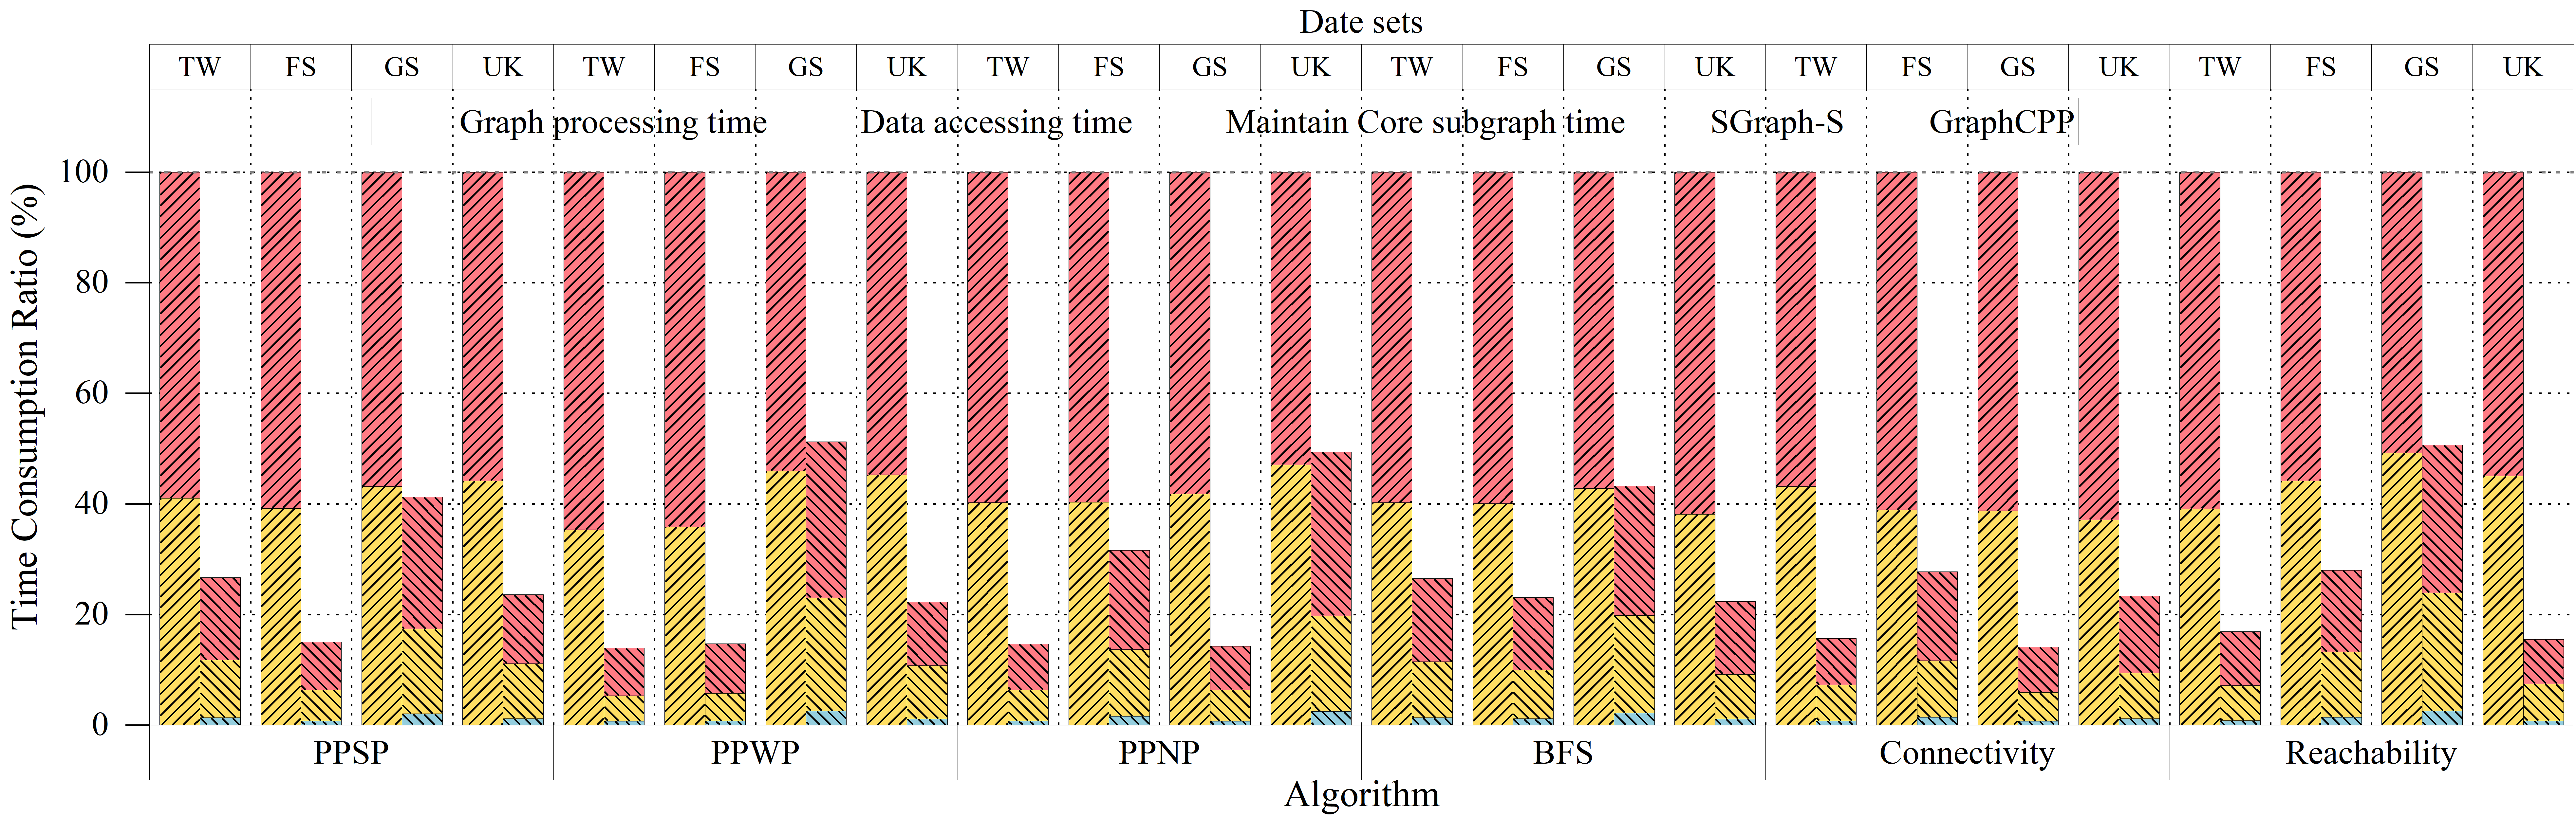
\includegraphics[width=7.0in, height=1.98in]{picture/Zhang-fig7.png}
    \captionsetup{labelsep=period}
    \caption{\centering{Computation Sharing Mechanism}}
    \label{fig7}
\end{figure*}

In Figure \ref{fig7}(a), we label vertices with connection edges exceeding 6 as {\bf{hot~vertices}}, considering the one with the highest degree as the Global Vertex, while the remaining hot vertices are allocated to the Core Subgraph.
Figure \ref{fig7}(b) depicts the operation of the {\bf{Global Vertices Mechanism}}, which computes query results from hot vertices to other vertices ($Q(v_6\rightarrow *)$) and from other vertices to hot vertices ($Q(*\rightarrow v_6$)) during the preprocessing stage.
This precomputation enables rapid determination of query bounds without actual computations when the query process traverses Global Vertices. For instance, before traversing the query $Q(v_1\rightarrow v_9)$, we can quickly establish a valid path connecting $v_1$ and $v_9$: $v_1\rightarrow v_6\rightarrow v_9$. At this point, $Q(v_1\rightarrow v_9) = R(v_1\rightarrow v_6) + R(v_6\rightarrow v_9)$. 
The right side of the equation represents the query results for $v_1$ to $v_6$ and $v_6$ to $v_9$, which are computed during the preprocessing stage. Using this equation, we obtain the bound for $Q(v_1\rightarrow v_9)$ without redundant computation, assisting subsequent iterative processes.
The computation sharing based on Global Vertices is termed as the first level of computation sharing. While the number of Global Vertices is often limited in practical applications due to their computational and storage costs, it also affects the efficiency of computation sharing. The subsequent Core Subgraph Mechanism addresses this limitation.

The {\bf{Core Subgraph Mechanism}} is illustrated in Figure \ref{fig7}(c). During the preprocessing stage, we identify hot vertices within the Core Subgraph and pair them to create vertex pairs for queries. For a given number of hot vertices, denoted as $m$ (in this instance, $m$ is 5), we generate $m \times m$ vertex pairs and utilize a table ($T_{subgraph}$) of this size to store their query results. We consider the converged query paths as edges in Core Subgraph, with the edge weights indicating the corresponding converged query results.
To keep operations lightweight, we do not directly compute the query results for these hot vertex pairs. Instead, during runtime, we extract hot path fragments from known query results. This is facilitated by a straightforward observation: \textit{if we acquire a converged query path between two vertices, any path fragment extracted from this path also satisfies the convergence condition}.
In the final part of this section, we elaborate on obtaining relevant information from converged paths, extracting hot path segments, and efficiently facilitating the sharing of query results for identical hot paths across different queries. As shown in Figure 7, leveraging the Core Subgraph allows us to break down $Q(v_1\rightarrow v_9)$ into $Q(v_1\rightarrow v_2) + R(v_2\rightarrow v_{10}) + R(v_{10}\rightarrow v_9)$, effectively avoiding redundant computations of $Q(v_2\rightarrow v_{10})$.
It is crucial to note that during querying, we lack knowledge on how to partition a complete query into multiple sub-queries. In practice, we treat edges in the Core Subgraph as normal outgoing edges. When a task traverses a vertex $v_i$ within the Core Subgraph, it considers other hot vertices in the Core Subgraph as outgoing neighbors of $v_i$, with the edge weights representing the corresponding query results. Therefore, for $Q(v_1\rightarrow v_9)$, $v_1$ initially traverses its outgoing neighbor $v_2$, then $v_2$ traverses its outgoing neighbor $v_{10}$, and finally, $v_{10}$ traverses its outgoing neighbor $v_9$. The entire process aligns with the normal traversal steps, rendering the Core Subgraph transparent to the user.
In contrast to the Global Vertices Mechanism, the Core Subgraph is more lightweight, encompassing more hot vertices and providing more precise pruning bounds.




\begin{algorithm}[t]
  \caption{Dual-level Computation Sharing Algorithm}
  \begin{algorithmic}[1]
    \Function{Preprocessing}{$V, k, m$}
      \State $V_{{global}}, V_{{subgraph}} \gets \text{StatisticsVertexDegree}(V, k, m)$
      \State $T_{{global}}^s,T_{{global}}^d \gets \text{ComputeGlobalVertices}(V_{{global}})$
      \State $T_{{subgraph}} \gets \text{InitCoreSubgraph}(V_{{subgraph}})$
    \EndFunction
    \Function{ComputationSharing}{$B$, $Q_{similar}$}
      \For{\textbf{each} $q_i$ \textbf{in} $Q_{similar}$ \textbf{in parallel}}
        \State $bound \gets \text{L1Share}(T_{{global}}, {q_i})$
        \State $V_{{active}} \gets \text{GetActiveVertexSet}({q_i})$
        \For{\textbf{each} $v_i$ \textbf{in} $V_{{active}}$}
          \If{$v_i \in V_{{subgraph}}$}
            \State $bound \gets \text{L2Share}(v_i, T_{{subgraph}},bound)$
          \EndIf
          \State $bound \gets \text{travNeighbors}(v_i, V_{{active}}, bound)$
        \EndFor
      \EndFor
      \State \textbf{return} $V_{{active}}$
    \EndFunction
    \Function{MaintainCoreSubgraph}{$R$}
      \State $T_{{subgraph}} \gets \text{ExtractHotPath}(R)$
      \State \textbf{return} $T_{{subgraph}}$
    \EndFunction    
  \end{algorithmic}
\end{algorithm}
Algorithm 2 illustrates the steps of the dual-level computation sharing. It is broadly divided into three phases: the preprocessing phase (lines 1-5), which is responsible for collecting vertex degrees, precomputing Global Vertices, and initializing the Core Subgraph. The computation sharing phase (lines 6-18) achieves the first level of computation sharing through Global Vertices mechanism (line 8) and the second level through the Core Subgraph (line 12). The phase of Maintaining the Core Subgraph (lines 19-22) involves extracting hot paths from existing computation results into the Core Subgraph, thereby reducing redundant computations for subsequent queries.
The first stage is executed only once at the beginning of the query, while the latter two stages are iteratively executed throughout the entire runtime. Below are explanations of key functions in the algorithm.

{\bf{Preprocessing.}} 
Instead of using a complex evaluation method \cite{china2}, we opt for a simple yet effective approach by selecting a subset of vertices with the highest degree of incoming and outgoing edges in the graph as hot vertices. In the preprocessing stage, we utilize the selection sort algorithm to identify the top 522 vertices with the highest degree. We designate the top 10 vertices as Global Vertices and allocate the remaining 512 vertices to the Core Subgraph (line 2).
For the Global Vertices mechanism, employ a point-to-all query algorithm to obtain all query results for paths originating from or leading to Global Vertices.
This generates $k*|V|*2$ computation results, where $k$ represents the number of Global Vertices, and $|V|$ represents the total number of vertices in the graph.
We utilize $T_{global}^s$ to store all query results with Global Vertices as source, and $T_{global}^d$ to store those with Global Vertices as destination. The row and column indices of the table correspond to the starting and ending points of the query, facilitating the quick retrieval of the corresponding query results (line 3).
For the Core Subgraph mechanism, it contains $m$ vertices, allowing the formation of $m*m$ unique vertex pairs, with each pair corresponding to a single query result. We use a dedicated two-dimensional table $T_{subgraph}$ to store these results. Unlike the Global Vertices mechanism, the Core Subgraph only establishes the table and initializes it with empty values during preprocessing. In the third stage, it extracts hot paths from the previously computed query results to populate the Core Subgraph (line 4).



{\bf{Computation Sharing.}} 
In the computation sharing mechanism, we execute all queries concurrently (line 7).
{\bf{First layer of computation sharing}}: when a query $Q(v_s\rightarrow v_d)$ starts, the \texttt{L1Share()} function traverses $T_{global}^d$ to find all query results $R{(v_s,*)}$ corresponding to the row of $v_s$, and traverses $T_{global}^s$ to find all query results $R{(*,v_d)}$ corresponding to the column of $v_d$. Then, it iterates through all Global Vertices $v_h$ to obtain the minimum value of $R{(v_s,v_h)}+R{(v_h,v_d)}$.
This value serves as the query's bound, which can be utilized for pruning (line 8). This bound is continuously updated in successive iterations. If the query's start and end points are unreachable, the bound is set to infinity. The system then retrieves query information to obtain the corresponding active vertex set (line 9).
{\bf{Second layer of computation sharing}}: as mentioned above, various queries frequently recalculate certain popular paths. The Core Subgraph is utilized to share the query results for these hot paths. 
When traversing the hot vertex $v_h$ within the Core Subgraph, we initially explore $T_{subgraph}$ to retrieve all query results corresponding to the row of $v_h$. Each entry in this row represents a query result for a pair of vertices, where the row index denotes the starting vertex and the column index denotes the destination vertex. If there are non-empty entries in this row, it indicates that before the current query execution, another task traversed the corresponding path segment, obtaining and storing the relevant query result. This enables us to retrieve all non-empty query results from $v_h$ to other hot vertices. We consider these hot vertices as out-edge neighbors of $v_h$, and the query results between them as the edge weights. These edges serve as shortcuts, reducing redundant computations for hot paths and accelerating traversal (line 12).
Then, the query iterates over the neighbors of each query task, updating the bound and the next round of active vertex set (line 14).
Finally, the function returns the updated set ($V_{{active}}$) for the next round of computation (line 17).

{\bf{Maintain Core Subgraph.}} 
The first two stages initialize and utilize the Core Subgraph, respectively. This phase refines the query results of Core Subgraph in $T_{subgraph}$.
In monotonic point-to-point query algorithms, any path fragment of a convergent path does remain convergent itself. For instance, if we obtain the shortest path between two vertices, any fragment of that path corresponds to the shortest path between those vertices.
After completing a batch of queries, we analyze the composition of the convergent paths corresponding to the queries. If a known optimal query path contains multiple hot vertices, it implies the presence of at least one convergent path fragment consisting of hot vertices at both ends.
So, how do we obtain convergent path information? 
As the query path traverses a vertex $v_i$, we record the query result for the path $v_s\rightarrow v_i$ and the parent node of $v_i$ on this path. This information is retained until a new and better path reactivates $v_i$, at which point all information is updated. In this way, when the final query converges, we obtain the query results and parent nodes for each relevant vertex. 
Then, starting from the destination vertex ($v_d$), we extract the query results from the starting vertex to $v_d$ and its corresponding parent node along the convergent path. We then repeat the previous step with the obtained parent node until we obtain the complete convergent path from $v_s$ to $v_d$. Once this extraction process is complete, we update the query results in $T_{subgraph}$ at their corresponding positions to facilitate sharing in the next batch of queries.
It's essential to note that due to the pruning operations employed in point-to-point queries, effectively avoiding a significant portion of redundant calculations, the proportion of activated vertices is minimal. Consequently, the process of extracting hot path query results can be completed with extremely low time and space overhead.



\vspace{-8pt}
\section{EXPERIMENTAL EVALUATION}\label{experimental}
%This section presents experimental evaluation of GraphSO in comparison with state-of-the-art solutions.

\vspace{-4pt}
\subsection{Experimental Setup}
{\bf{Hardware Configuration.}} The experiments are conducted on an 8-node cluster, each machine equipped with 2 32-core lntel Xeon platinum 8358 CPUs (each CPU has 48MB L3 cache) and 256 GB memory. All nodes are interconnected through an lnfiniband network with a bandwidth of 300Gbps. The programs are compiled using gcc version 9.4.0, openMPl version 4.0.3, and with openMP enabled.


{\bf{Graph Algorithms And Datasets.}} 
We utilized six commonly used point-to-point query algorithms, as shown in Table \ref{table1}. These algorithms have broad applications in different domains, such as social networks and traffic planning, making them representative. Additionally, Table \ref{table3} provides details on the graph datasets used in these algorithms. The datasets cover diverse application scenarios and scales, following a power-law distribution that accurately reflects the characteristics of real-world graph distributions. 
We adopt advanced graph partitioning approach \cite{china1} to meet the requirements of distributed systems.

\begin{table}[h]
    \centering
    \renewcommand\arraystretch{1.2}
    \scriptsize
    \begin{tabular}{c c c c}
    \hline
    \rule{0pt}{8pt} 
    Datasets          & Vertices & Edges  & Data sizes \\
    \hline
    \rule{0pt}{8pt}
    Twitter-2010(TW) \cite{twitter}   & 41.7M    & 1.5B   & 10.9GB     \\
    Friendster(FS) \cite{Friendster}    & 65.6M     & 1.81B    & 8.7GB      \\
    Gsh-2015-host(GS) \cite{bubing}  & 68.7M    & 1.8B   & 13.4GB     \\
    UK-2007-05(UK) \cite{timeaware}     & 106M     & 3.74B  & 27.9GB     \\
    \hline
    \end{tabular}
    \caption{\centering{Graph Dataset Information}}
    \label{table3}
    \vspace{-0.3cm}
\end{table}

{\bf{System Comparison.}} We conducted a comparative analysis between GraphCPP and the state-of-the-art point-to-point query solution SGraph \cite{sgraph}. Additionally, we implemented a concurrent query processing version of SGraph, denoted by the `-C' suffix, and a sequential query execution version, denoted by the `-S' suffix.
To ensure scientific rigor in our experiments, we used random parameters for each query, maintaining consistency with the baseline: the number of Global Vertices was set to 10, and the vertices of the Core Subgraph in GraphCPP were set to 512. All tests were conducted 10 times, and the reported results represent the average values.


\vspace{-8pt}
\subsection{Overall Performance Comparison}
\vspace{-2pt}
\begin{figure*}[ht]
	\centering
	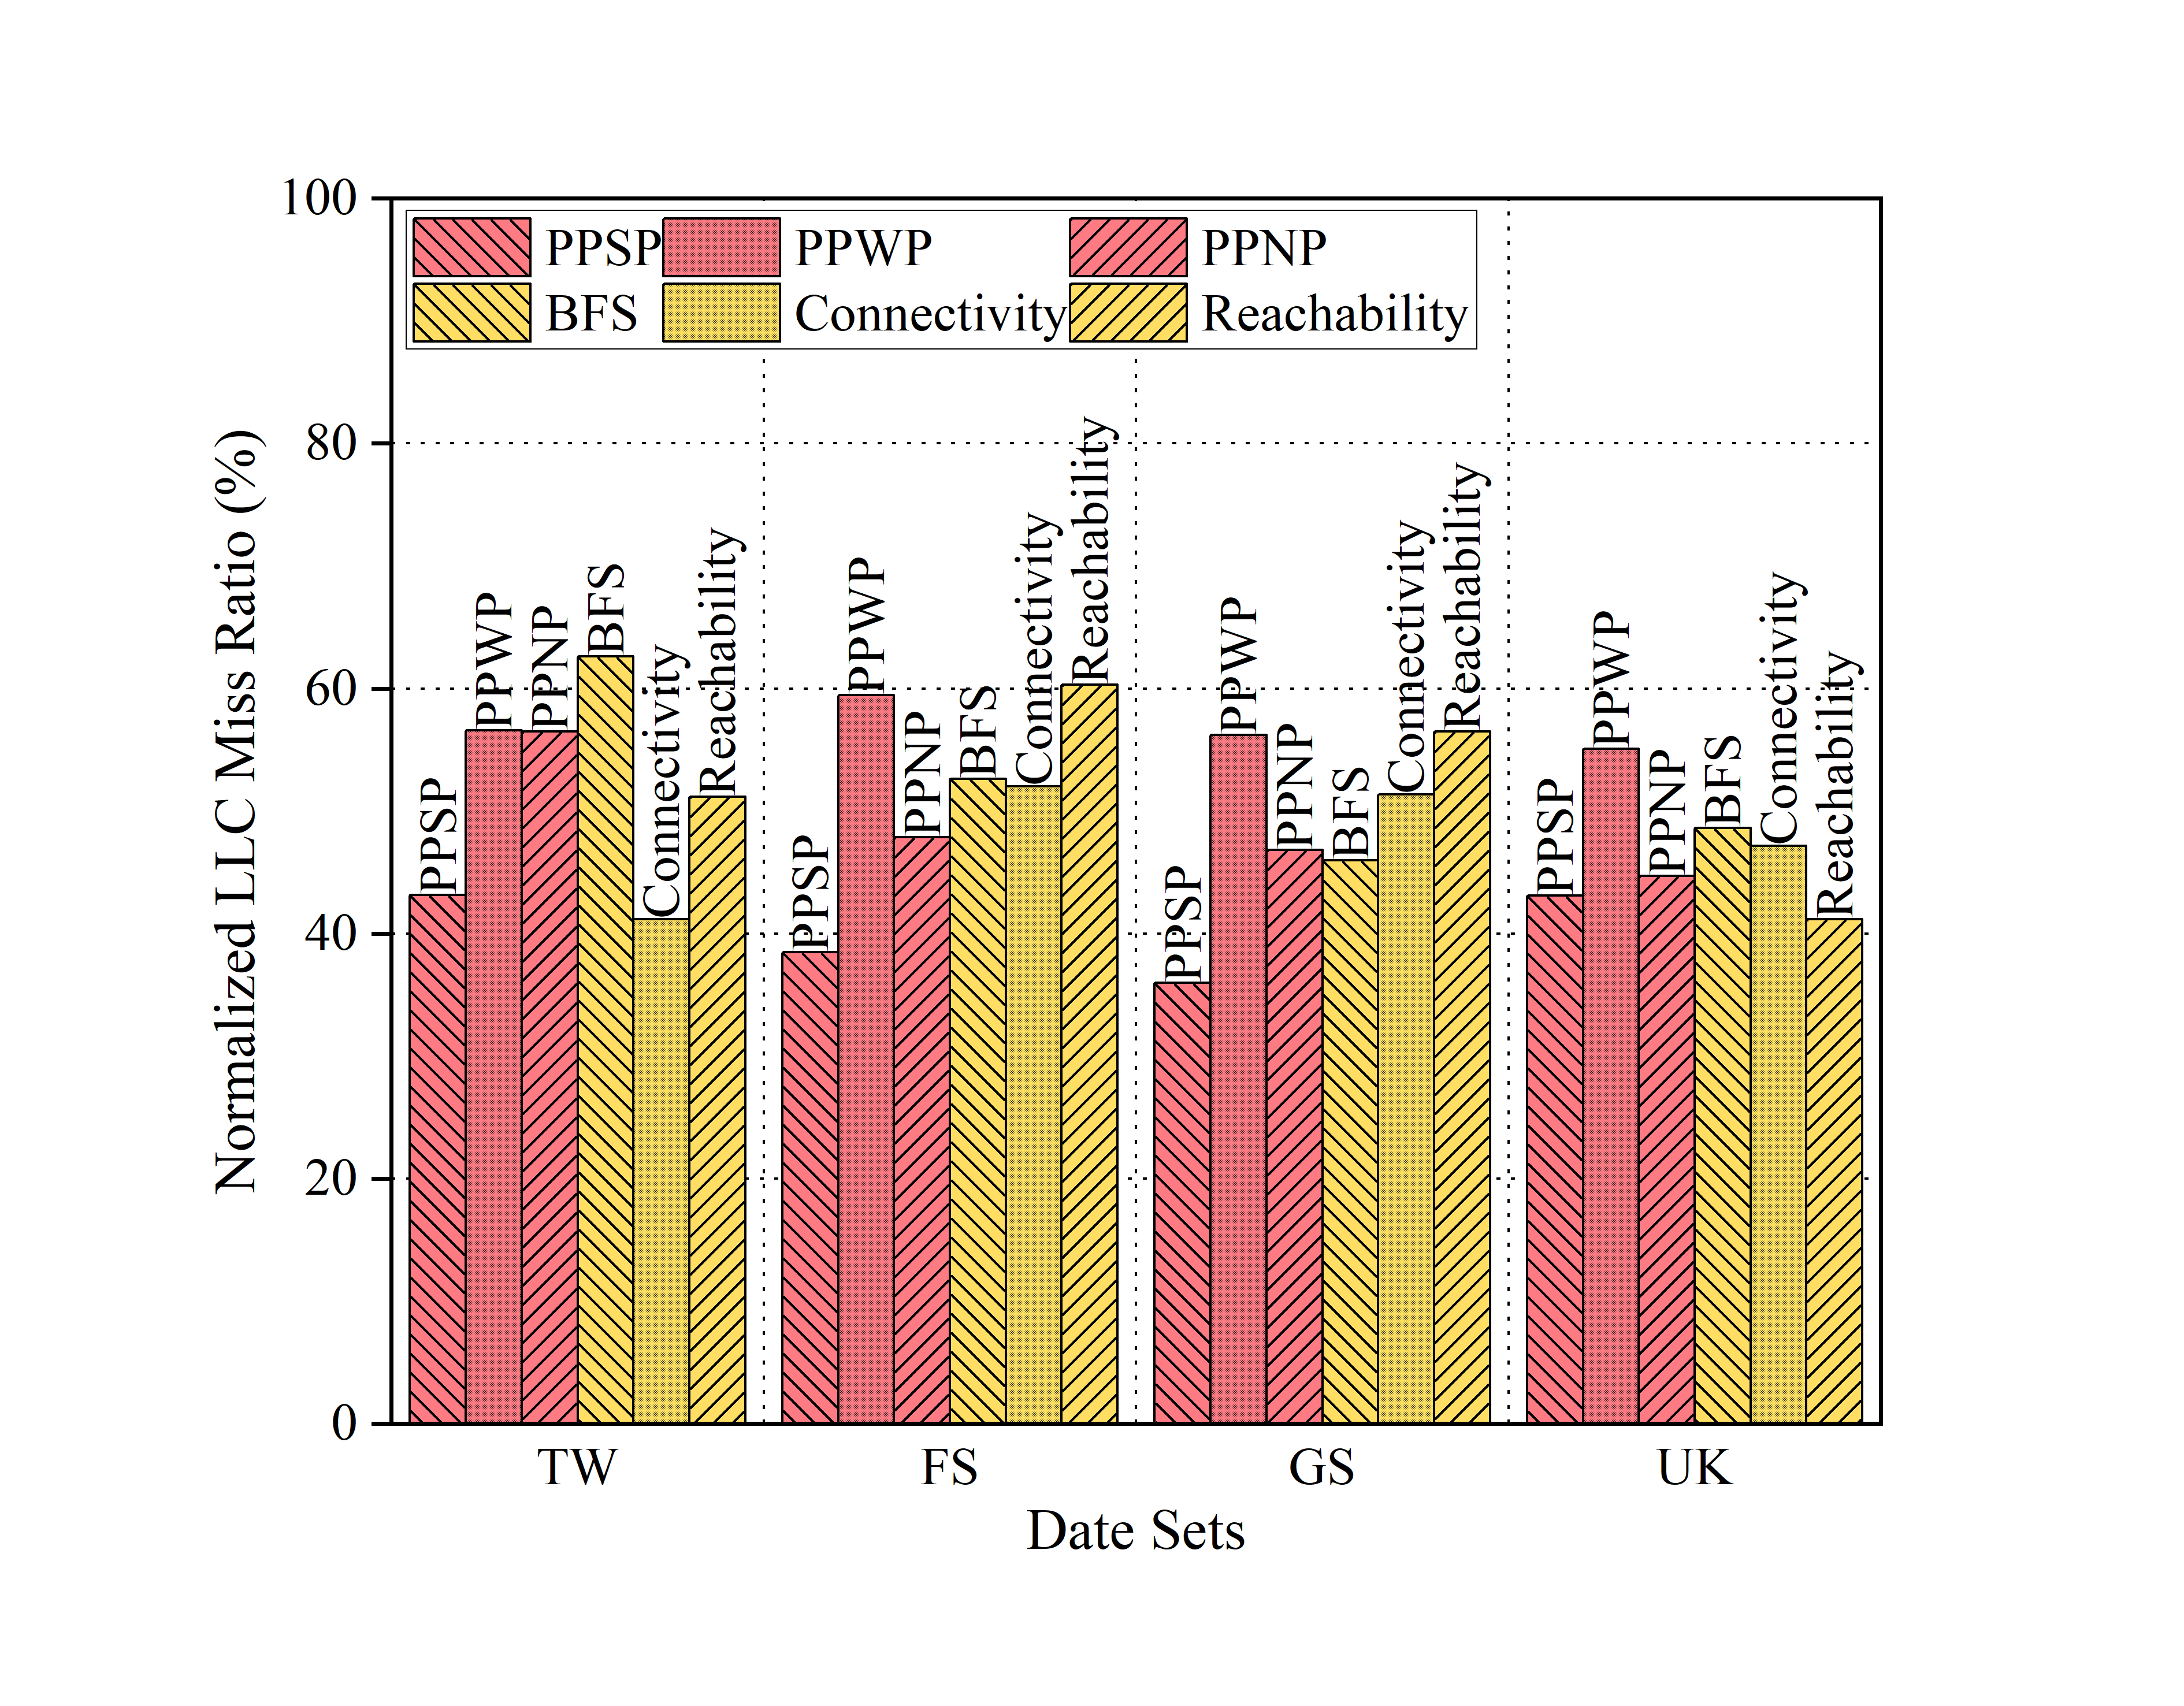
\includegraphics[width=7.0in, height=2.0in]{picture/Zhang-fig8.png} %调节单个子图大小
	%\setlength{\abovecaptionskip}{-0.05cm} %控制标题与子图距离
    \captionsetup{labelsep=period}
		\caption{\centering{Total execution time of different systems with six algorithms on four datasets (512 queries, 128 concurrent, normalized to SGraph-S)}} %子图下标题
		\label{fig8} %引用标签
\end{figure*}%

\begin{figure*}[ht]
	\centering
	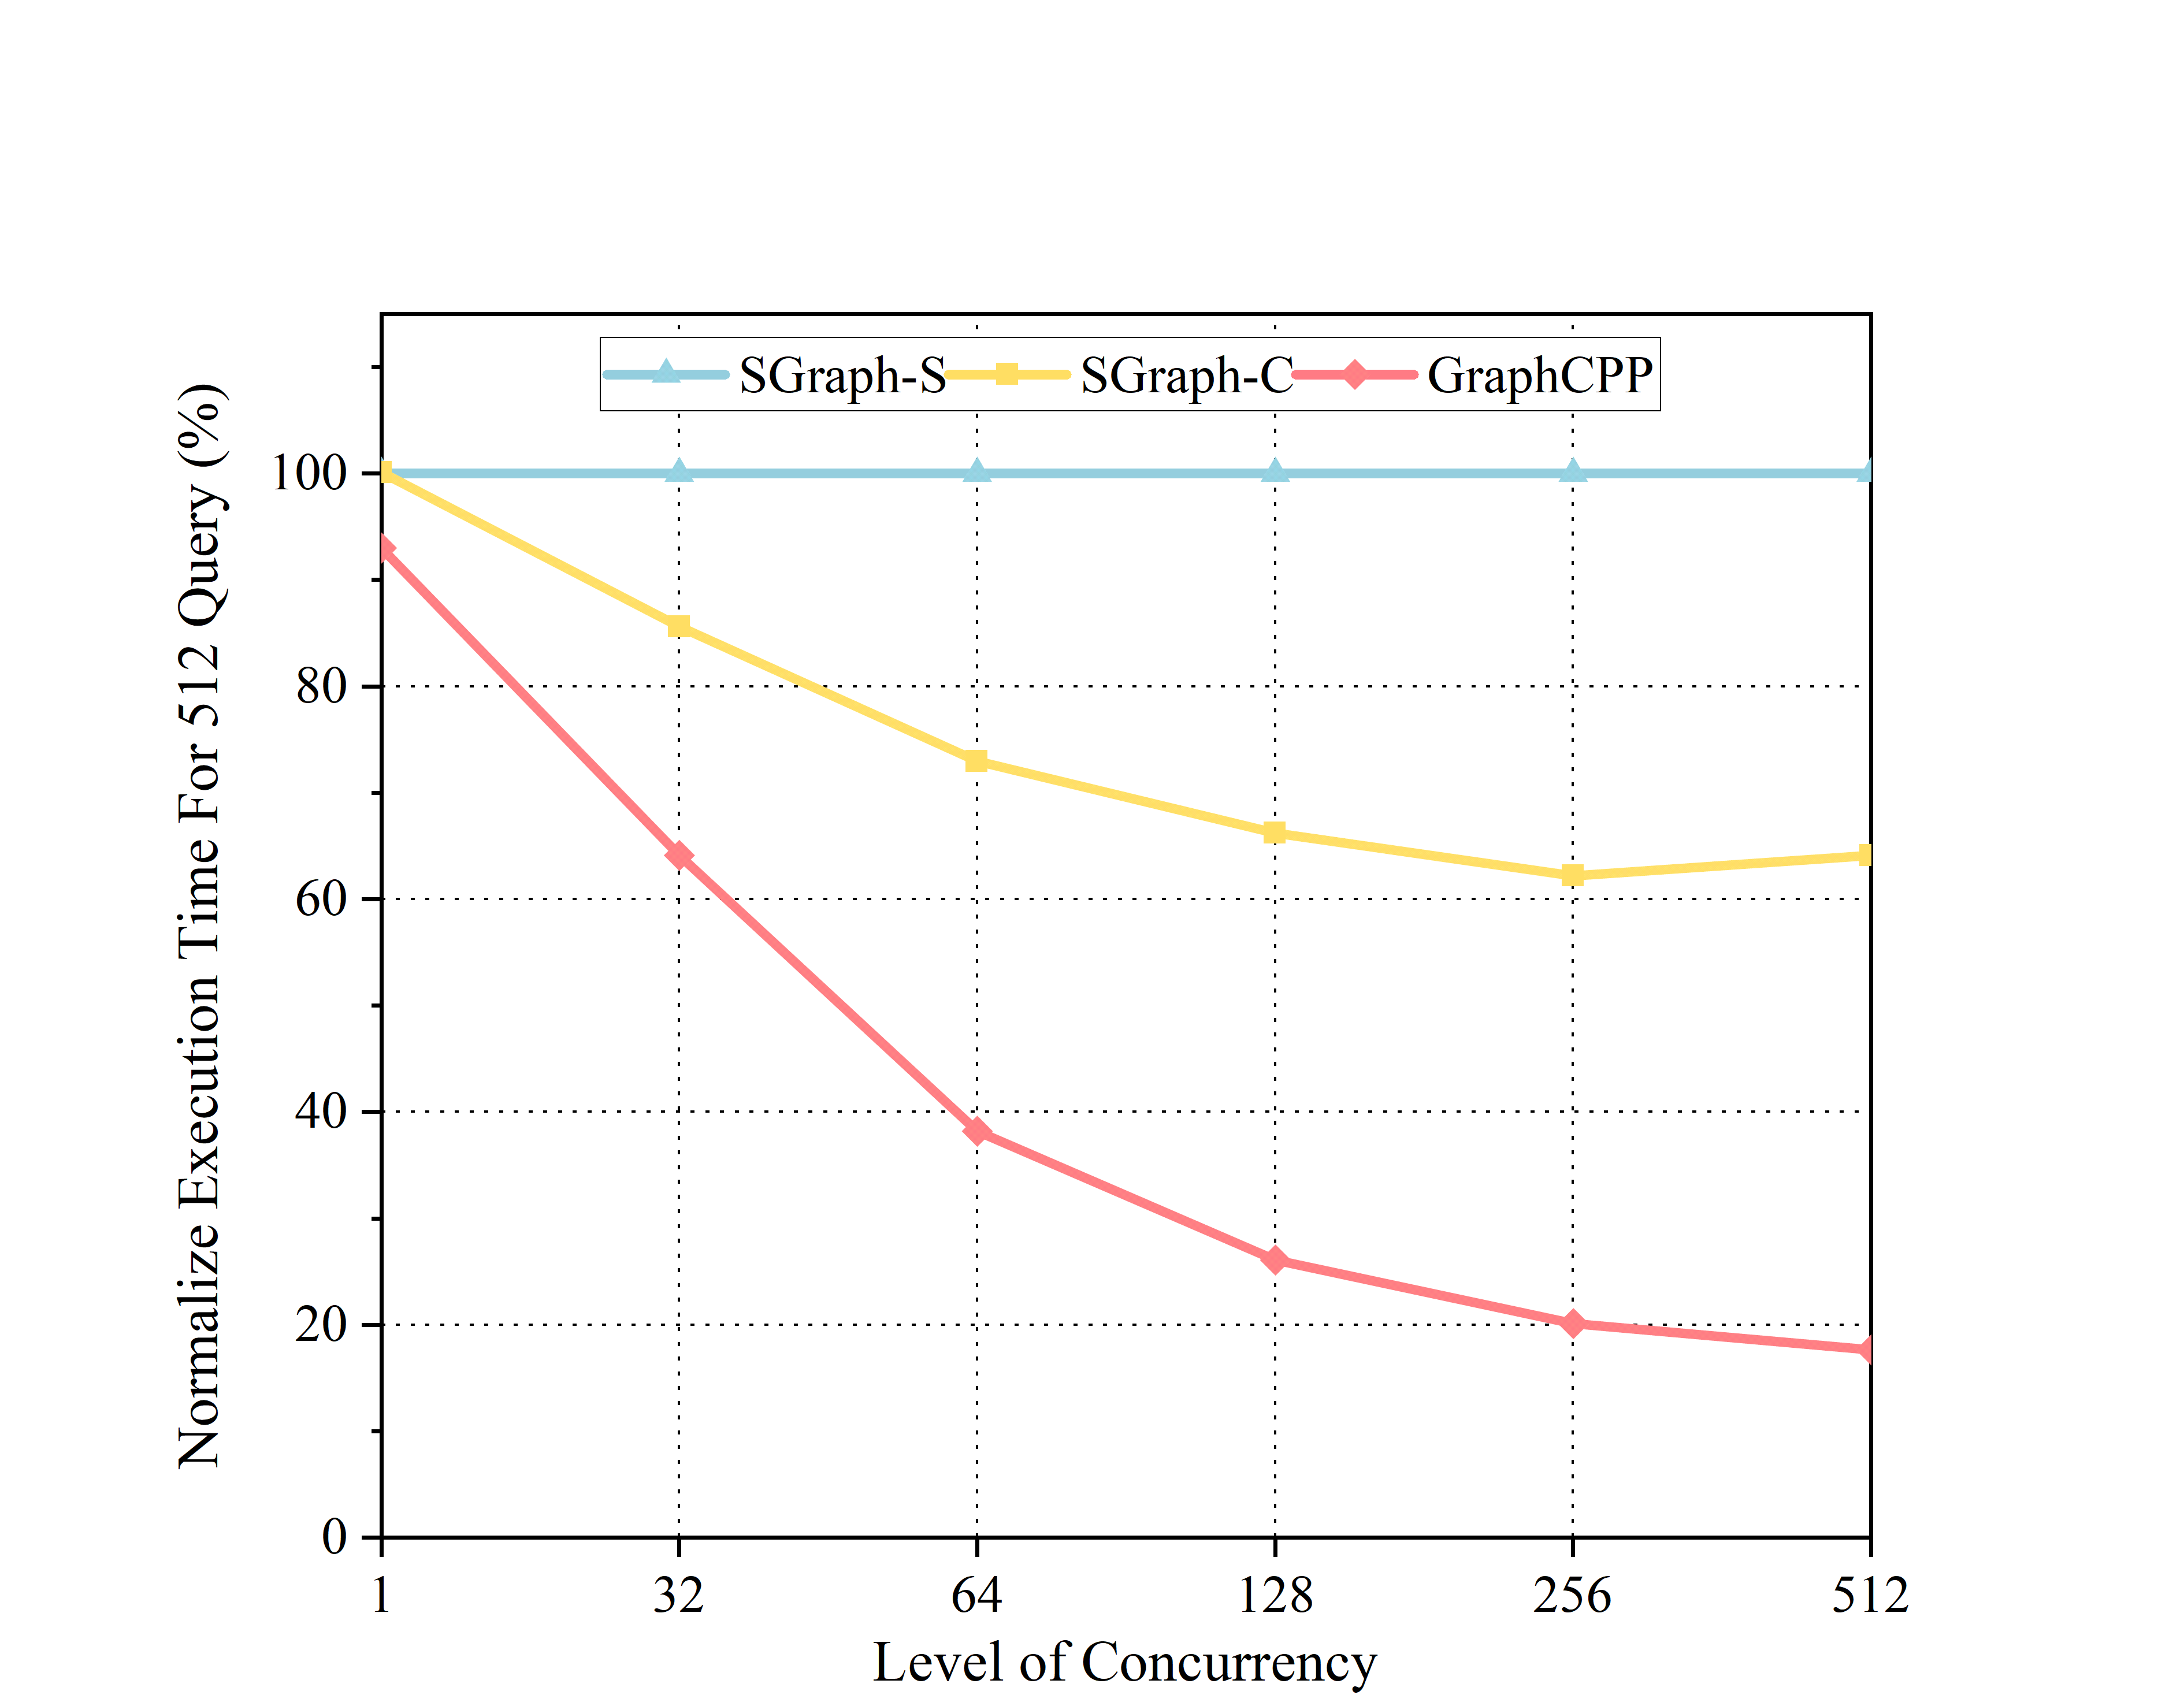
\includegraphics[width=7.0in, height=2.0in]{picture/Zhang-fig9.png}
	%\setlength{\abovecaptionskip}{-0.05cm} 
    \captionsetup{labelsep=period}
		\caption{\centering{Execution time breakdown of different systems with six algorithms on four datasets (512 queries, 128 concurrent, normalized to SGraph-S)}}
		\label{fig9}
\end{figure*}



\begin{figure}[ht]
    \centering
	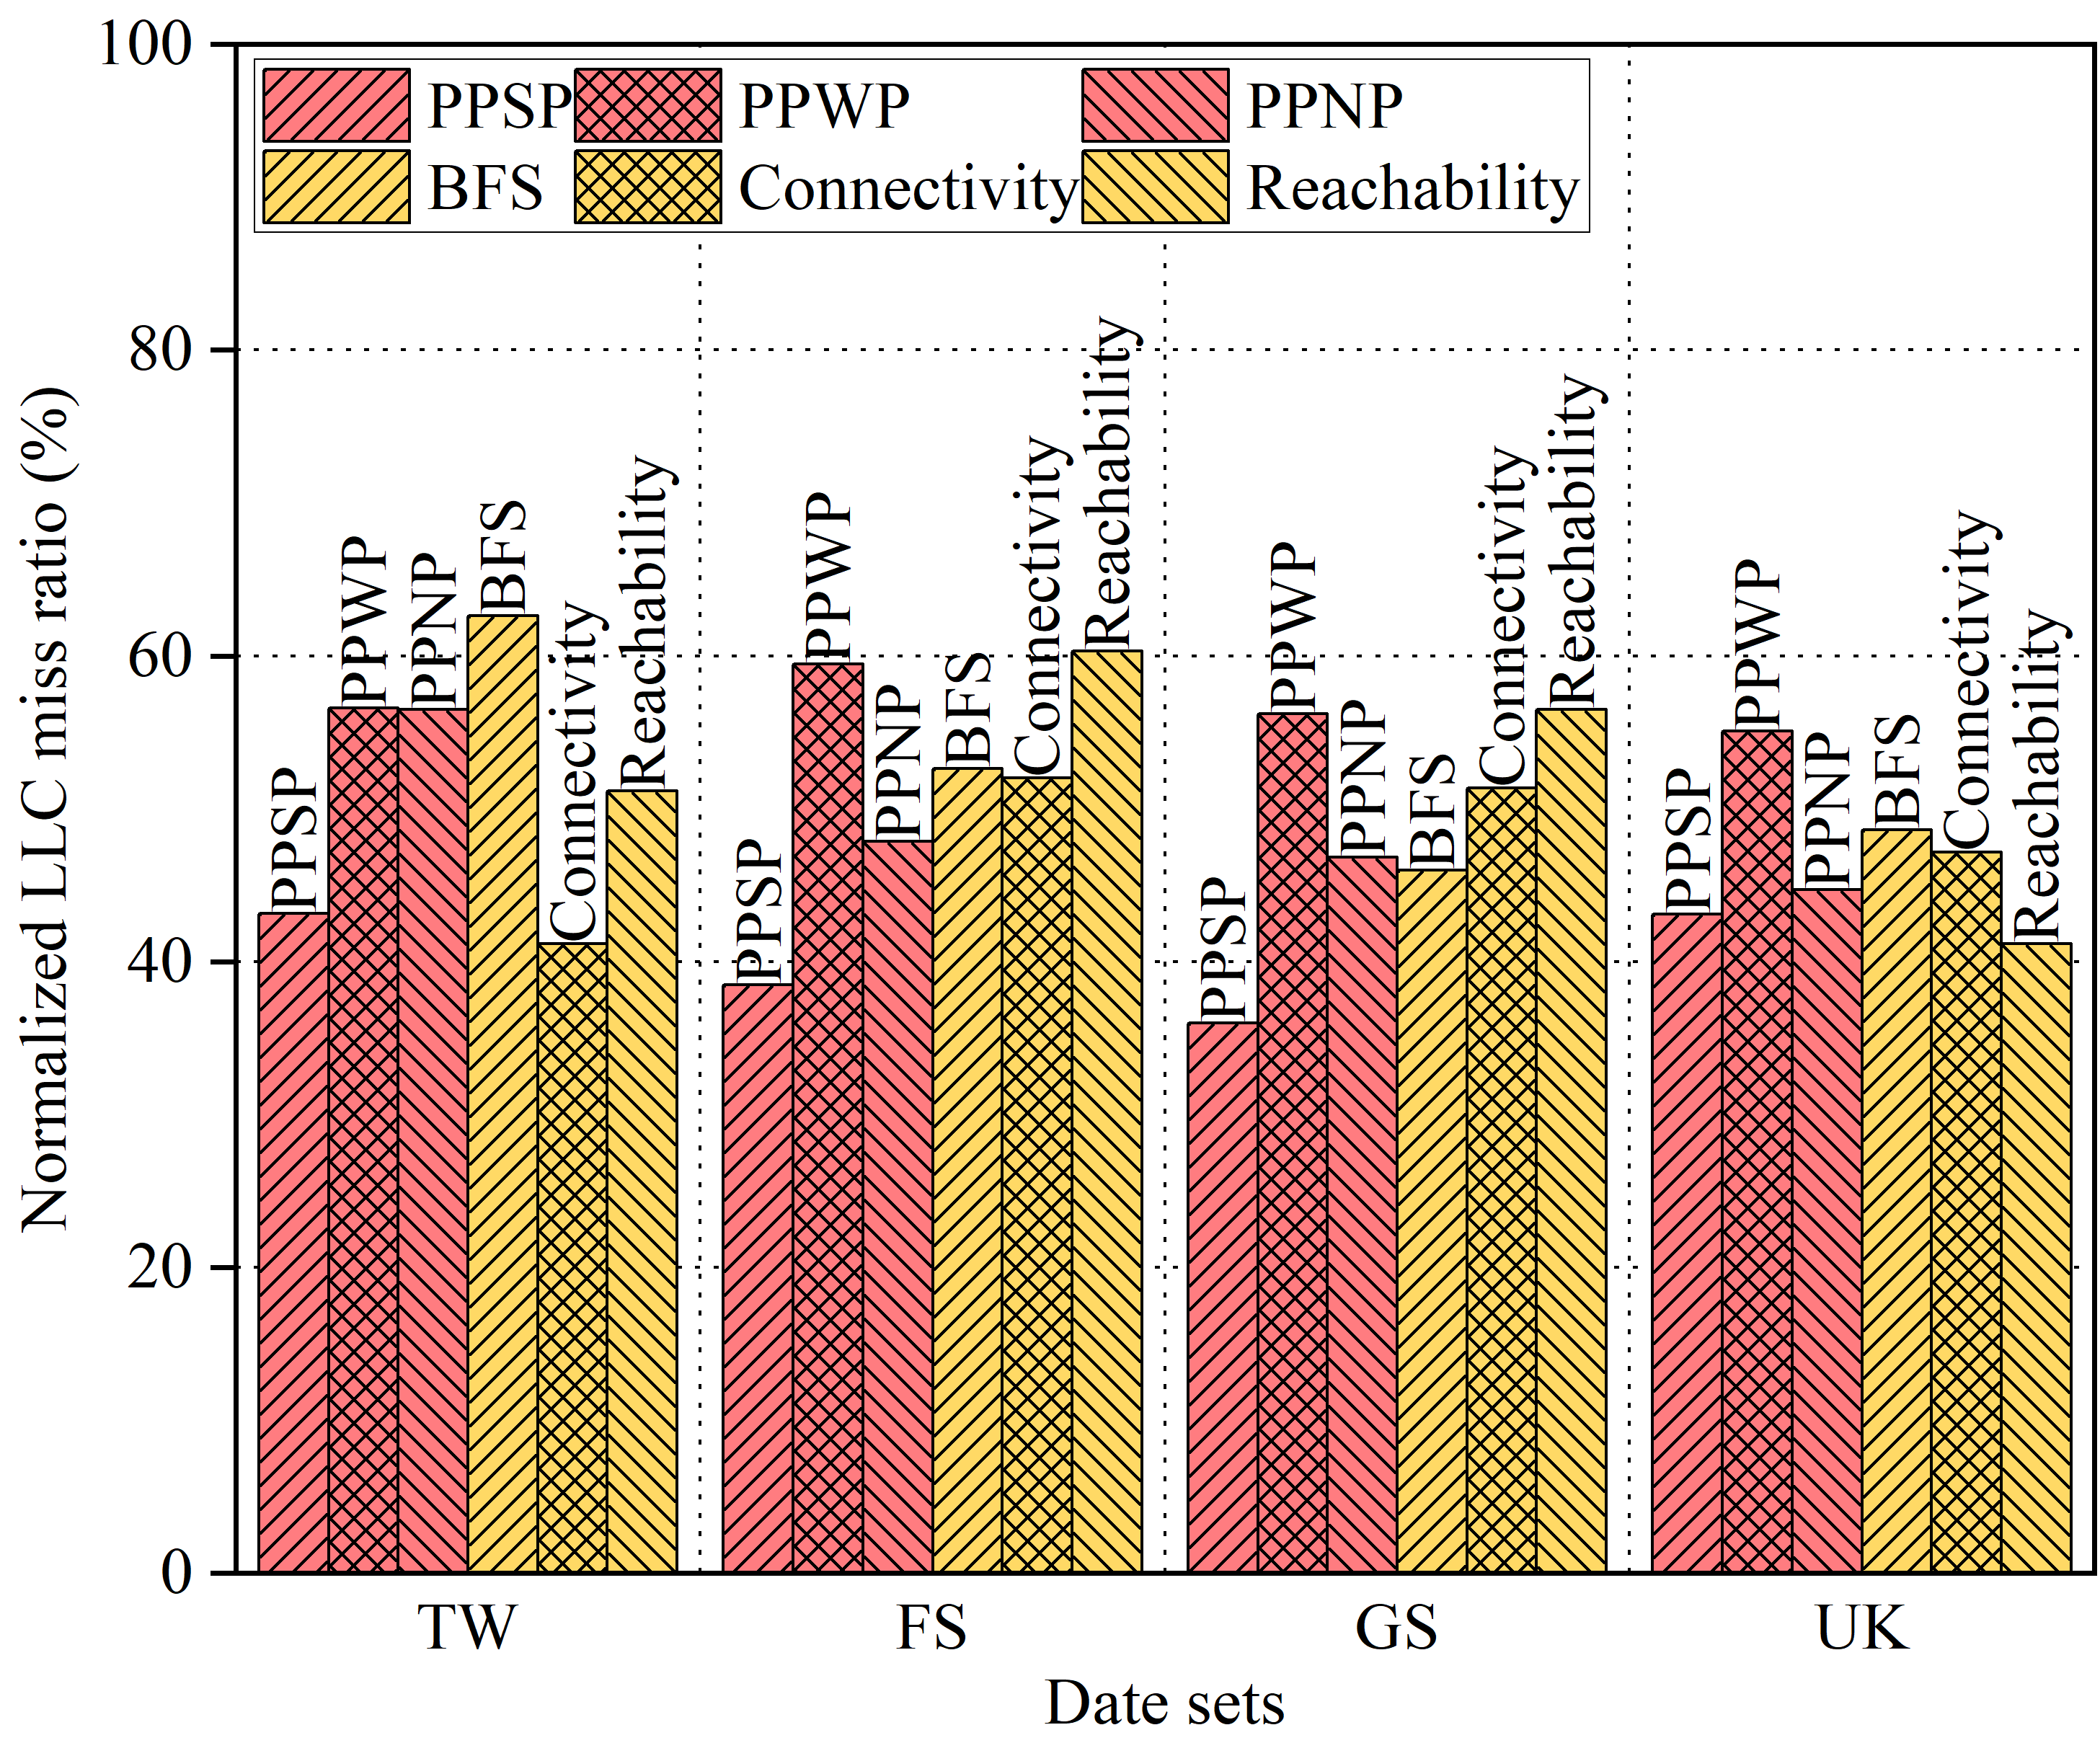
\includegraphics[width=3.0in, height=2.0in]{picture/Zhang-fig10.png}
	%\setlength{\abovecaptionskip}{-0.05cm} 
    \captionsetup{labelsep=period}
		\caption{\centering{LLC miss rate of GraphCPP with six algorithms on four datasets (512 queries, 128 concurrent, normalized to SGraph-S)}}
		\label{fig10}
    \vspace{-0.4cm}
\end{figure}

Figure \ref{fig8} illustrates the overall execution time for 512 queries using various approaches. The execution time is normalized relative to the performance of SGraph-S, considering significant variations in the execution time across different test cases. The results indicate that GraphCPP consistently achieves shorter execution time for all graphs and algorithms. Specifically, when compared to alternative schemes, GraphCPP demonstrates an average throughput improvement ranging from 1.56 to 5.67 times. This improvement is attributed to the reduction of data access costs and effective pruning of the Core Subgraph in GraphCPP.


For a more detailed performance analysis, we further categorize the total time into data access time and graph processing time, measured by the waiting time for core pauses. As depicted in Figure \ref{fig9}, GraphCPP requires less time for graph data access compared to SGraph-S, with this proportion decreasing as the graph size increases. Notably, GraphCPP's data access time averages a reduction of 1.23 to 2.39 times when compared to other systems. The efficiency of GraphCPP stems from two critical factors: 1) identical portions of graph data required by different concurrent queries are loaded and maintained as a single copy in memory, reducing overall memory consumption; 2) graph data blocks are prioritized and regularly loaded into the LLC based on associated query counts, facilitating job reuse and effectively lowering LLC miss rates, thereby minimizing unnecessary memory data transfers. Furthermore, the two-level computing sharing mechanism contributes to GraphCPP's lower computation time compared to other systems.



\vspace{-10pt}
\subsection{Efficiency of Data Access Sharing Mechanism}
\vspace{-2pt}
In Figure \ref{fig9}, GraphCPP demonstrates a substantial reduction in data access time, ranging from 45\% to 85\%, when utilizing the data access sharing mechanism compared to SGraph. This performance improvement is attributed to concurrent tasks sharing the data access overhead, and the unified scheduling approach of the data access sharing mechanism enhances data locality for various tasks. To assess the effectiveness of our data-sharing mechanism, we conducted 512 queries on the different graph and normalized GraphCPP's LLC miss ratio relative to SGraph-S. As shown in Figure \ref{fig10}, GraphCPP consistently achieves a lower LLC miss ratio across all datasets and algorithms, averaging a 50\% improvement.


\vspace{-8pt}
\subsection{Efficiency of the Computation Sharing Mechanism}
\vspace{-2pt}
We compared the performance of GraphCPP and SGraph-S (Figure \ref{fig9}), demonstrating that despite the inherent overhead of the computation sharing mechanism (including the cost of computing Global Vertices and maintaining the Core Subgraph), an overall computational acceleration is achieved. The specific costs associated with this mechanism are outlined below:

{\bf{Global Vertices Overhead.}} GraphCPP and SGraph-S both require precomputation and storage of queries involving Global Vertices in the graph, facilitating shared calculations for any computation that involves Global Vertices. The computation and storage overhead for Global Vertices is proportionate to the number of Global Vertices. For SGraph, it needs to maintain a sufficient number of Gobal Vertices (usually 16) to ensure the efficiency of computation sharing. However, for GraphCPP, it achieves this by initializing query boundaries based on Global Vertices, and more precise boundaries can be established in subsequent Core Subgraph computations. This flexibility enables GraphCPP to select fewer Global Vertices query results without compromising the efficiency of computation sharing. For instance, reducing the number of Global Vertices from 16 to 10 can result in a 37.5\% reduction in the computation and storage overhead associated with Global Vertices.

{\bf{Core Subgraph Overhead.}} We designed the construction of the Core Subgraph to leverage previous query results, employing a lightweight prefix sum method for extracting hot paths. As depicted in Figure \ref{fig8}, the time dedicated to maintaining the Core Subgraph constitutes approximately 5\% of GraphCPP's total execution time. Despite this, it significantly reduces the overall computation time. Additionally, for each hot path, we need to store its query result and the vertices it traverses. We observe a positive correlation between the number of Core Subgraph vertices and storage overhead. Nevertheless, this cost remains relatively small when compared to the overall graph size since the Core Subgraph exclusively stores paths among hot vertices, and the maximum number of hot paths is merely the square of the hot vertices, making it quite limited compared to larger graphs.

\begin{figure}[t]
    \centering
    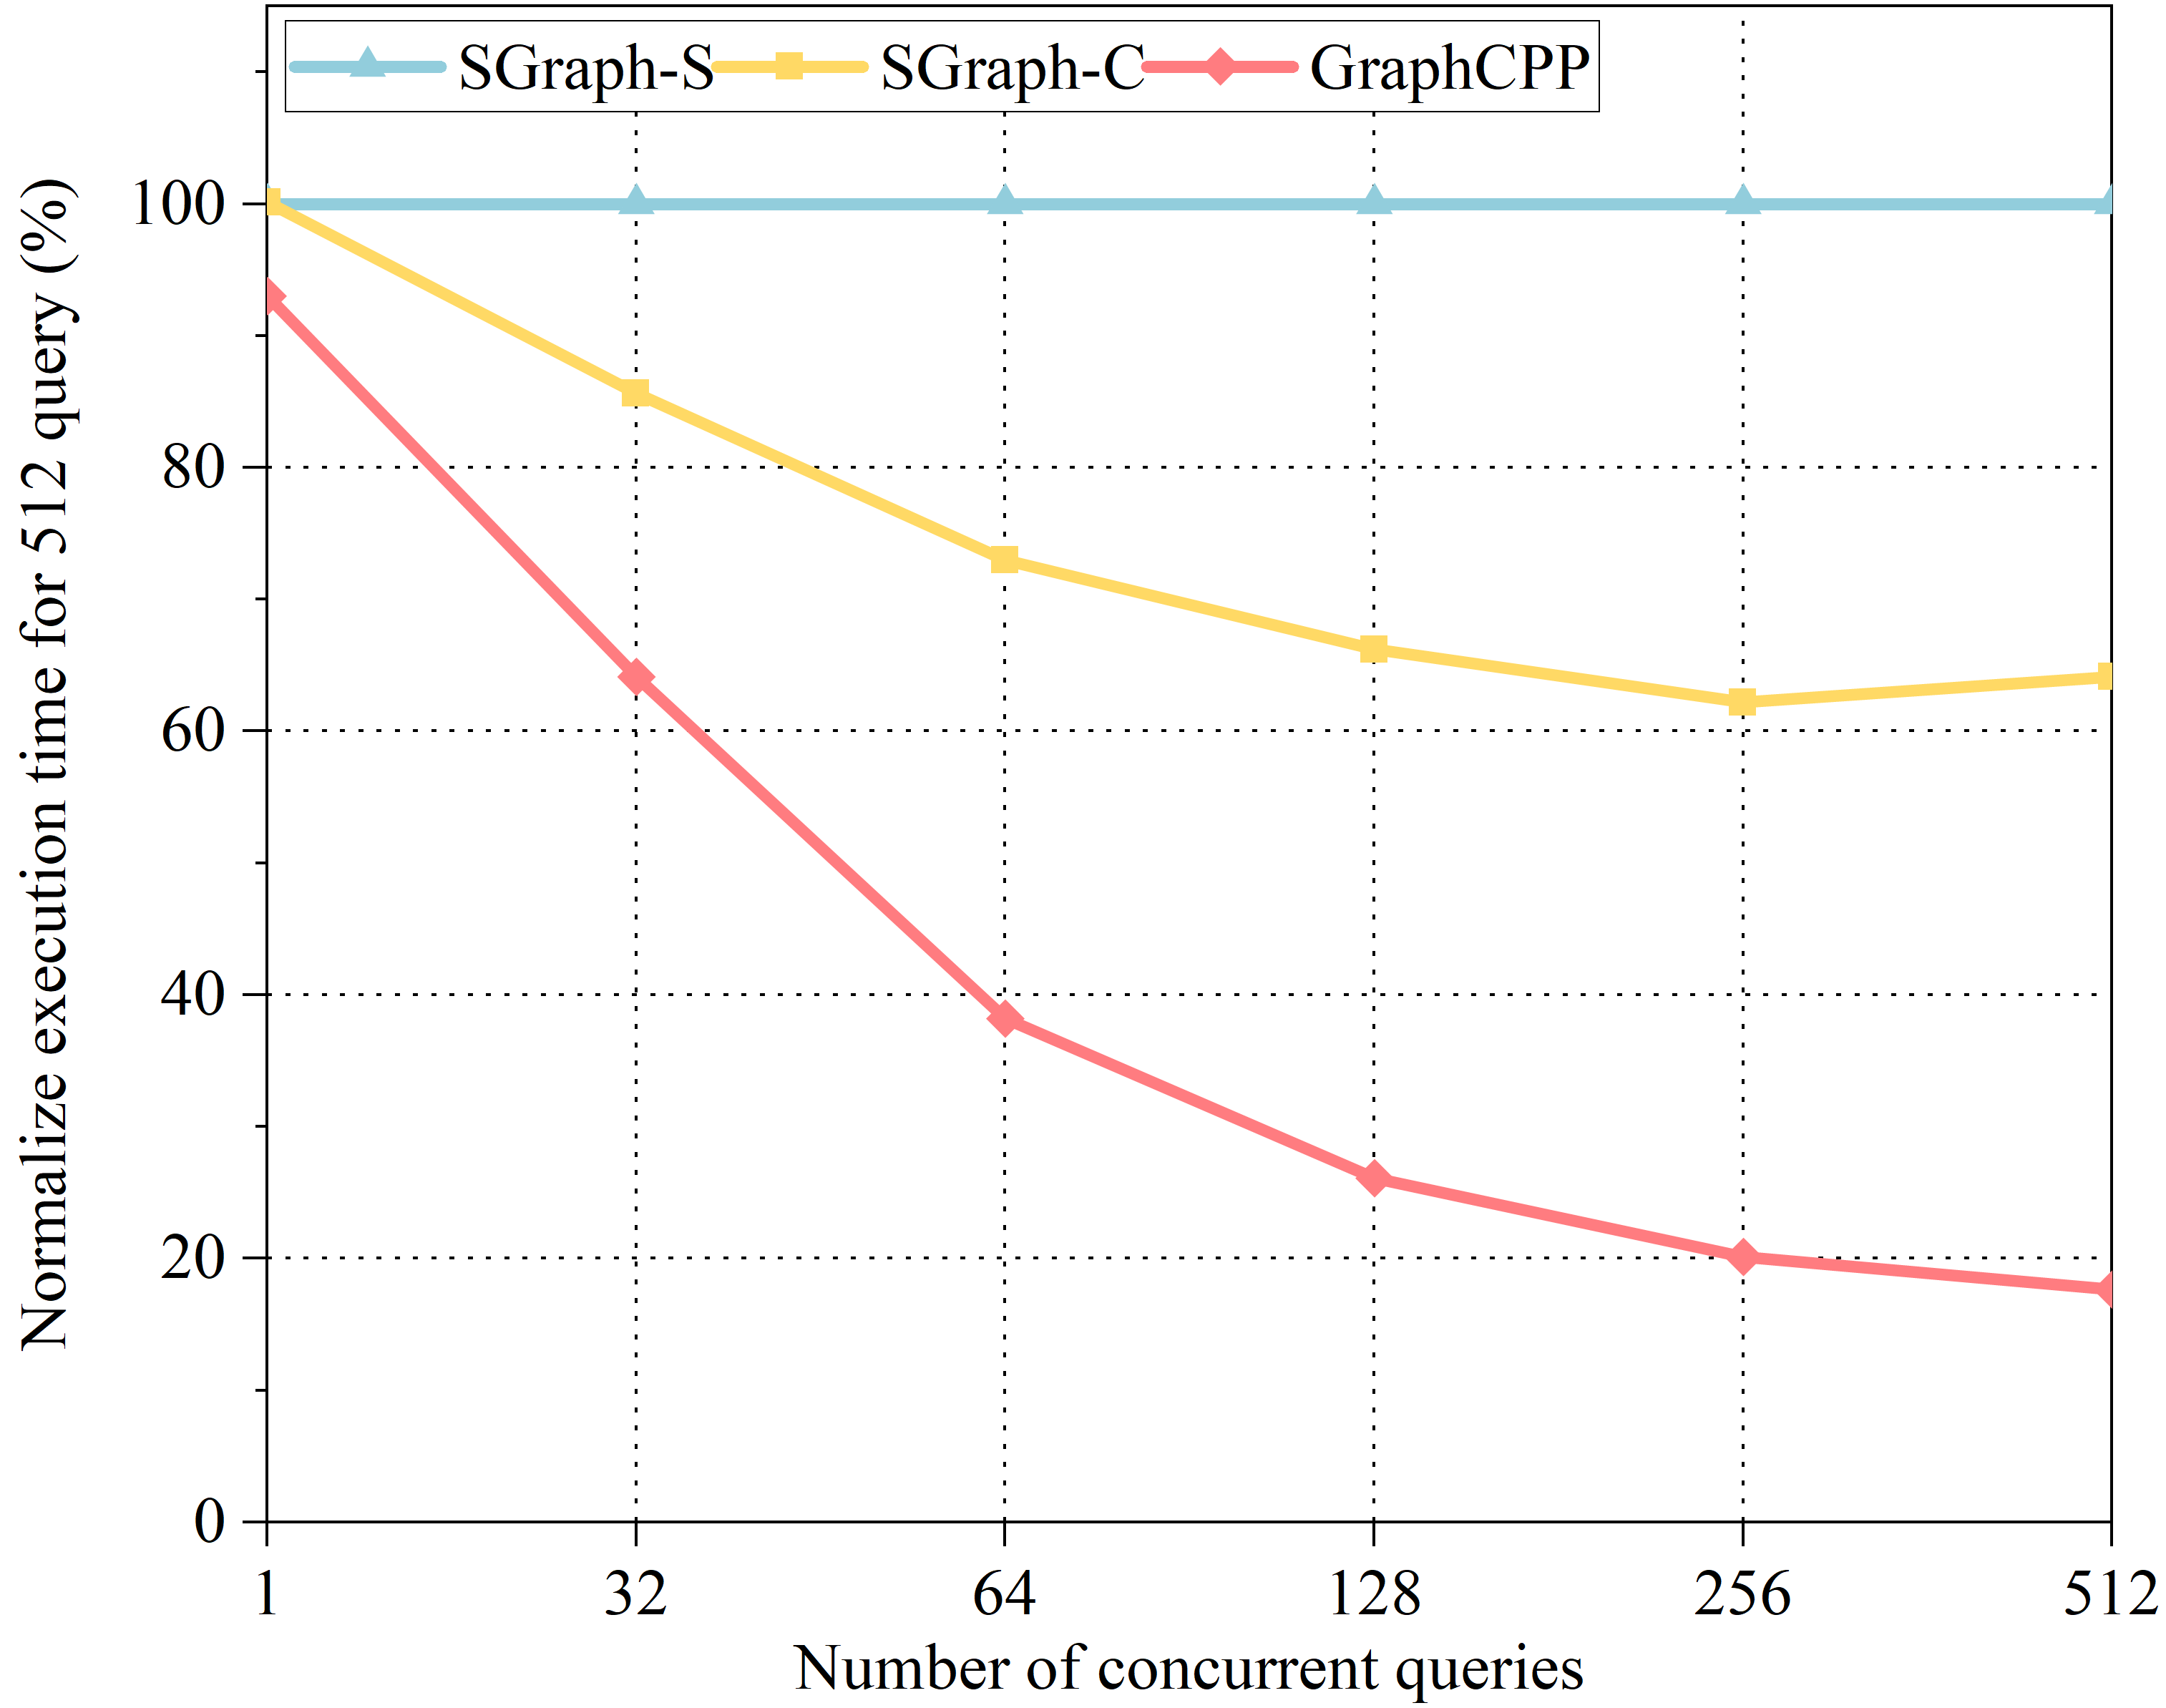
\includegraphics[width=3.0in, height=2.0in]{picture/Zhang-fig11.png}
    %\setlength{\abovecaptionskip}{-0.05cm} 
    \captionsetup{labelsep=period}
    \caption{\centering{Scalability of different systems with varying concurrency (512 PPSP queries on TW \cite{twitter}, normalized to SGraph-S)}}
    \label{fig11}
    \vspace{-0.5cm}
\end{figure}

\vspace{-8pt}
\subsection{Scalability of GraphCPP}
\vspace{-4pt}
In Figure \ref{fig11}, we evaluated the scalability of different systems by examining the time required for 512 queries under different concurrent query counts.
For clearer comparison, we normalized the query time of SGraph-C and GraphCPP relative to SGraph-S. The blue horizontal line represents the time required for SGraph-S to linearly execute 512 queries.
We chose the maximum of 512 concurrency, indicating that all queries can be completed in a single concurrent execution.
SGraph-C benefits from concurrent execution; however, the absence of a data sharing mechanism results in the highest synchronization overhead among concurrent tasks, resulting in an earlier performance turning point. As the concurrent count increases, the performance gains diminish gradually.
In comparison, GraphCPP consistently exhibits a decrease in processing time. This is attributed to its efficient data access and computation sharing mechanism, which consequently reduce the overhead of individual query task, enhancing the system's scalability to concurrent query tasks.


\vspace{-8pt}
\section{RELATED WORK}\label{relate_work}
{\bf{Graph Processing Systems}}. Graph computation systems fall into three main categories based on differences in storage media and computing platforms.
1) Single-node in-memory systems: Ligra \cite{ligra} optimizes graph traversal using push-pull computation. GraphBolt \cite{graphbolt} and ACGraph \cite{acgraph} handle streaming graphs incrementally. DiGraph \cite{digraph} supports iterative directed graph processing on GPUs. DepGraph \cite{depgraph} and TDGraph \cite{tdgraph} reduce redundancy and data access costs through topology-aware execution.
2) Single-node out-of-core systems: FlashGraph \cite{flashgraph} achieves high IOPS with semi-external memory. GridGraph \cite{gridgraph} enhances locality with Streaming-Apply. DGraph \cite{efficient} accelerates processing through faster state propagation. GraphM \cite{graphm} optimizes throughput for concurrent systems.
3) Distributed systems: Pregel \cite{pregel} uses Bulk Synchronous Parallel (BSP) for scalable, fault-tolerant processing of large graphs. PowerGraph \cite{powergraph} reduces communication volume with vertex-cut partitioning. PowerLyra \cite{powerlyra} employs a hybrid model for high/low-degree vertices. Gemini \cite{gemini} ensures scalability with a dual-mode engine. CGraph \cite{cgraph} minimizes overhead with a load-trigger-push (LTP) model.
However, existing graph computing systems mainly focus on point-to-all algorithms, which are not suitable for point-to-point scenarios.

{\bf{Point-to-Point Queries}}. Numerous studies have explored point-to-point queries. For example, $Hub^2$ \cite{hub} introduces a specialized hardware accelerator that utilizes a hub-centric approach to constrain the search scope of high-degree vertices, thereby expediting the PPSP process. Quegel \cite{quegel} pursues a software-based query result sharing approach, improving response speed by constructing a static distributed query-sharing table during loading. PnP \cite{pnp} adopts a universal pruning strategy to reduce redundant accesses and computations. Tripoline \cite{tripoline} combines query reuse and pruning, achieving incremental query evaluation without prior knowledge through the application of the triangle inequality principle. Although initially designed for point-to-all algorithms, it can also be applied to point-to-point query systems.
SGraph \cite{sgraph} further optimizes pruning strategies by incorporating upper and lower bounds, resulting in sub-second latency queries on large graphs with dynamically changing data.
Existing solutions focus on improving the speed of individual point-to-point queries by pruning or sharing results. But they often overlook optimizing throughput in concurrent queries by sharing data access. Additionally, some approaches utilize the Global Vertices mechanism to achieve computation sharing. This approach requires exponential storage, computation, and dynamic upkeep as the graph size grows. To alleviate high overhead, practitioners often limit the number of vertices, which compromises the efficiency of computation sharing.


{\bf{Concurrent Graph Computing}}. Concurrent graph processing systems address large-scale data across diverse architectures. Single-node in-memory system like Congra \cite{Congra}, enhances throughput and resource efficiency through dynamic query scheduling and awareness of atomic operations. Krill \cite{krill} adopts an SAP model to simplify attribute data management and reduce memory access. ForkGraph \cite{cache} accelerates execution by employing a yield-based scheduling strategy for efficient data sharing among concurrent queries. Out-of-core systems, such as GraphM \cite{graphm} and its distributed counterpart CGraph \cite{cgraph}, exploit locality to facilitate effective data sharing and computation.
Other out-of-core systems, including Seraph \cite{seraph}, advocates for decoupling data structures, while MultiLyra \cite{multilyra} optimizes batch query evaluation by distributing communication costs through graph and boundary sharing. While the previously mentioned systems concentrate on optimizing data access sharing for concurrent general algorithms, they overlook specific optimizations for point-to-point queries.

\section{CONCLUSION}\label{conclusion}
Traditional point-to-point query systems excel in optimizing individual queries, but encounter throughput challenges in large-scale concurrent query scenarios. In contrast, contemporary concurrent graph computing systems have extensively explored the concurrent execution of point-to-all algorithms. However, due to the absence of efficient pruning mechanisms, they demonstrate low efficiency in handling point-to-point queries. GraphCPP identifies substantial redundancies in data access and computation among concurrent point-to-point queries, which brings optimization opportunities. It introduces a data-driven caching execution mechanism to facilitate overlapping data access sharing during concurrent queries. Additionally, it employs a two-level computation sharing mechanism, effectively enabling computation sharing across multiple queries. Experimental results indicate that GraphCPP achieves a performance improvement of 3.2x on average compared to existing state-of-the-art approach.

\section{ACKNOWLEDGMENTS}\label{acknowledfments}
This paper is supported by National Key Research and Development Program of China (No. 2022YFB2404202), Key Research and Development Program of Hubei Province (No. 2023BAB078), Knowledge Innovation Program of Wuhan-Basi Research (No. 2022013301015177), and Huawei Technologies Co., Ltd (No. YBN2021035018A6).

%\vspace{-10pt}
% use section* for acknowledgment
\ifCLASSOPTIONcompsoc
% The Computer Society usually uses the plural form
%\section*{Acknowledgments}
%\else
% regular IEEE prefers the singular form
%\section*{Acknowledgment}
%\fi
%This paper is supported by National Key Research and Development Program of China under grant No. 2018YFB1003500, National Natural Science Foundation of China under grant No.~61832006, 61825202, and 61702202. This work is also supported by Science and Technology on Parallel and Distributed Processing Laboratory (PDL).
\vspace{-8pt}
% Can use something like this to put references on a page
% by themselves when using endfloat and the captionsoff option.
\ifCLASSOPTIONcaptionsoff
  \newpage
\fi


\begin{thebibliography}{100}
\bibliographystyle{IEEEtran}
\bibitem{google}
``Google Maps,'' https://www.alibabagroup, 2023.

\bibitem{facebook}
``Facebook,'' www.facebook.com, 2023.

\bibitem{alipay}
``Alipay,'' www.alipay.com, 2019.

\bibitem{pnp}
C. Xu, K. Vora, R. Gupta, ``Pnp: Pruning and prediction for point-to-point iterative graph analytics,'' in \textit{Proc. Int. Conf. Architectural Support Program. Languages Operating Syst.}, Providence, RI, USA, 2019, pp. 587--600.

\bibitem{sgraph}
H. Chen, M. Zhang, K. Yang, et al., ``Achieving Sub-second Pairwise Query over volving Graphs,'' in \textit{Proc. Int. Conf. Architectural Support Program. Languages Operating Syst.}, Vancouver, BC, Canada, 2023, pp. 1--15.

\bibitem{tripoline}
X. Jiang, C. Xu, X. Yin, et al., ``Tripoline: generalized incremental graph processing via graph triangle inequality,'' in \textit{Proc. Eur. Conf. Comput. Syst.}, United Kingdom, 2021, pp. 17--32.

\bibitem{glign}
X. Yin, Z. Zhao, and R. Gupta, ``Glign: Taming Misaligned Graph Traversals in Concurrent Graph Processing,'' in \textit{Proc. ACM Int. Conf. Architectural Support Program. Languages Operating Syst.}, Vancouver, BC, Canada, 2022, pp. 78--92.


\bibitem{cagis}
``Cagis,'' http://www.cagis.org.cn, 2021.

\bibitem{Friendster}
``Stanford large network dataset collection,'' http://snap.stanford.edu/data/index.html, 2020.

\bibitem{twitter}
H. Kwak, C. Lee, H. Park, et al., ``What is Twitter, a social network or a news media?'' in \textit{Proc. Int. Conf. World Wide Web}, Raleigh, NC, USA, 2020, pp. 591--600.

\bibitem{bubing}
P. Boldi, A. Marino and M. Santini, et al.,  ``BUbiNG: Massive Crawling for the Masses,''  \textit{ACM Trans. Web}, vol. 12, no. 2, pp. 1--26, 2018.

\bibitem{timeaware}
P. Boldi, M. Santini and S. Vigna,  ``A large time-aware web graph,''  \textit{ACM SIGIR Forum}, vol. 42, no. 2, pp. 33--38, 2008.

\bibitem{ppsp}
K. Joseph, H. Jiang, ``Content based News Recommendation via Shortest Entity Distance over Knowledge Graphs,'' in \textit{Companion Proc. 2019 World Wide Web Conf.}, San Francisco, CA, USA, 2019, pp. 690--699.

\bibitem{ppwp}
M. Pollack, ``The maximum capacity through a network,'' \textit{Operations Res.}, Vol. 8, no. 5, pp. 733--736, 1960.

\bibitem{ppnp}
O. Berman, G. Handler, ``Optimal Minimax Path of a Single Service Unit on a Network to Nonservice Destinations,'' \textit{Transp. Sci.}, Vol. 21, no. 2, pp. 115--122, 1987.

\bibitem{bfs}
S. Schaeffer, ``Graph clustering,'' \textit{Comput. Sci. Rev.}, Vol. 1, no. 1, pp. 27--64, 2020.

\bibitem{connectivity}
L. Dhulipala, C. Hong, J. Shun, ``A framework for static and incremental parallel graph connectivity algorithms,'' \textit{arXiv preprint arXiv:2008.03909}, 2020. 

\bibitem{reachability}
E. Cohen, E. Halperin, H. Kaplan, et al., ``Reachability and Distance Queries via 2-Hop Labels,'' \textit{SIAM J. Comput.}, Vol. 32, no. 5, pp. 1338--1355, 2003.

\bibitem{ligra}
J. Shun, J. Blelloch, ``Ligra: a lightweight graph processing framework for shared memory,'' in \textit{Proc. Symp. Princ. Pract. Parallel Program.}, Shenzhen, China, 2013, pp. 135--146.

\bibitem{graphbolt}
M. Mariappan, K. Vora, ``Graphbolt: Dependency-driven synchronous processing of streaming graphs,'' in \textit{Proc. EuroSys Conf.}, Dresden, Germany, 2019, pp. 1--16.

\bibitem{acgraph}
Z. Jiang, et al., ``ACGraph: Accelerating Streaming Graph Processing via Dependence Hierarchy,'' in \textit{2023 60th ACM/IEEE Design Automation Conference (DAC)}, IEEE, 2023.

\bibitem{digraph}
Y. Zhang, X. Liao, H. Jin, et al., ``DiGraph: An efficient path-based iterative directed graph processing system on multiple GPUs,'' in \textit{Proc. Int. Cinf. Architectural Support Program. Languages and Operating Syst.}, Providence, RI, USA, 2019, pp. 601--614.


\bibitem{depgraph}
Y. Zhang, X. Liao, H. Jin, et al., ``DepGraph: A Dependency-Driven Accelerator for Efficient Iterative Graph Processing,'' in \textit{IEEE Int. Symp. High-Perform. Comput. Architecture }, Seoul, Korea, 2021, pp. 371--384.

\bibitem{tdgraph}
J. Zhao, Y. Yang, Y. Zhang, et al., ``TDGraph: a topology-driven accelerator for high-performance streaming graph processing,'' in \textit{Proc. Annu. Int. Symp. Comput. Architecture}, New York, NY, USA, 2022, pp. 116--129.

\bibitem{flashgraph}
D. Zheng, M. Mhembere, R. Burns, et al., ``{FlashGraph}: Processing {Billion-Node} Graphs on an Array of Commodity {SSDs},'' in \textit{USENIX Conf. File Storage Technologies}, Santa Clara, CA, USA, 2015, pp. 45--58.

\bibitem{gridgraph}
X. Zhu, W. Han, W. Chen, ``{GridGraph}:{Large-Scale} Graph Processing on a Single Machine Using 2-Level Hierarchical Partitioning,'' in \textit{USENIX Annu. Tech. Conf.}, Santa Clara, CA, USA, 2015, pp. 375--386.

\bibitem{efficient}
Y. Zhang, X. Liao, X. Shi, et al., ``Efficient Disk-Based Directed Graph Processing: A Strongly Connected Component Approach,'' \textit{IEEE Trans. Parallel Distrib. Syst.}, vol. 29, no. 4, pp. 830--842, 2018.

\bibitem{graphm}
J. Zhao, Y. Zhang, X. Liao, et al., ``GraphM: an efficient storage system for high throughput of concurrent graph processing,'' in \textit{Proc. Int. Conf. High Perform. Comput., Netw., Storage and Anal.}, Denver, Colorado, USA, 2019, pp. 1--14.

\bibitem{pregel}
G. Malewicz, M. Austern, A. Bik, et al., ``Pregel: a system for large-scale graph processing,'' in \textit{Proc. ACM SIGMOD Int. Conf. Manage. Data}, New York, NY, USA, 2010, pp. 135--146.

\bibitem{cgraph}
Y. Zhang, J. Zhao, X. Liao, et al., ``{CGraph}: A Correlations-aware Approach for Efficient Concurrent Iterative Graph Processing,'' in \textit{USENIX Annu. Tech. Conf.}, Boston, MA, USA, 2018, pp. 441--452.

\bibitem{gemini}
X. Zhu, W. Chen, W. Zheng, et al., ``Gemini: A {Computation-Centric} Distributed Graph Processing System,'' in \textit{USENIX Symp. Operating Syst. Des. Implementation}, Savannah, GA, USA, 2016, pp. 301--316.

\bibitem{giraph}
C. Avery, ``Giraph: Large-scale graph processing infrastructure on hadoop,'' in \textit{Proc. Hadoop Summit}, pp. 5--9, 2011.

\bibitem{graphlab}
Y. Low, J. Gonzalez, A. Kyrola, et al., ``Graphlab: A new framework for parallel machine learning,'' \textit{arXiv preprint arXiv:1408.2041}, 2019.

\bibitem{powergraph}
J. Gonzalez, Y. Low, H. Gu, et al., ``{PowerGraph}: Distributed {Graph-Parallel} Computation on Natural Graphs,'' in \textit{USENIX Symp. Operating Syst. Des. Implementation}, Hollywood, CA, USA, 2012, pp. 17--30.

\bibitem{graphx}
J. Gonzalez, R. Xin, A. Dave, et al., ``{GraphX}: Graph Processing in a Distributed Dataflow Framework,'' in \textit{USENIX Symp. Operating Syst. Des. Implementation}, Broomfield, CO, USA, 2014, pp. 599--613.


\bibitem{powerlyra}
R. Chen, J. Shi, Y. Chen, et al., ``Powerlyra: Differentiated graph computation and partitioning on skewed graphs,'' \textit{ACM Trans. Parallel Comput.}, vol. 5, no. 3, pp. 1--39, 2019.

\bibitem{hub}
R. Jin, N. Ruan, B. You, et al., ``Hub-accelerator: Fast and exact shortest path computation in large social networks,'' \textit{arXiv preprint arXiv:1305.0507}, 2013.

\bibitem{quegel}
Q. Zhang, D. Yan and J. Cheng, ``Quegel: A general-purpose system for querying big graphs,'' in \textit{Proc. Int. Conf. Manage. Data}, New York, NY, USA, 2016, pp. 2189--2192.

\bibitem{Congra}
P. Pan and C. Li, ``Congra: Towards Efficient Processing of Concurrent Graph Queries on Shared-Memory Machines,'' in \textit{IEEE Int. Conf. Comput. Des.}, Boston, MA, USA, 2017, pp. 217--224.

\bibitem{krill}
H. Chen, M. Shen, N. Xiao, et al., ``Krill: a compiler and runtime system for concurrent graph processing,'' in \textit{Proc. Int. Conf. High Perform. Comput., Netw., Storage and Anal.}, New York, NY, USA, 2021, pp. 1--16.

\bibitem{cache}
S. Lu, S. Sun, J. Paul, et al., ``Cache-efficient fork-processing patterns on large graphs,'' in \textit{Proc. Int. Conf. Manage. Data}, New York, NY, USA, 2021, pp. 1208--1221.

\bibitem{seraph}
J. Xue, Z. Yang, Z. Qu, et al., ``Seraph: an efficient, low-cost system for concurrent graph processing,'' in \textit{Proc. Int. Symp. High-perform. Parallel Distrib. Comput.}, Vancouver, BC, Canada, 2014, pp. 227--238.

\bibitem{multilyra}
A. Mazloumi, X. Jiang, R. Gupta, ``Multilyra: Scalable distributed evaluation of batches of iterative graph queries,'' in \textit{IEEE Int. Conf. Big Data}, Los Angeles, CA, USA, 2019, pp. 349--358.

\bibitem{china1}
X. Liu, Z. Ji, T. Hou, ``Graph partitions and the controllability of directed signed networks,'' in \textit{Sci. China Inf. Sci}, vol. 62, no. 4, pp. 1--11, 2019.

\bibitem{china2}
J. Zhang, H. Chen, D. Yu, et al., ``Cluster-preserving sampling algorithm for large-scale graphs,'' in \textit{Sci. China Inf. Sci}, vol. 66, no. 1, pp. 1--17, 2023.

\end{thebibliography}

% \vspace{-1.5cm}
% \begin{IEEEbiography}
% [{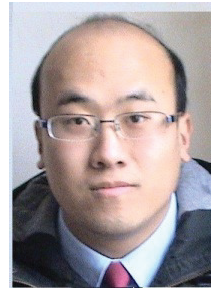
\includegraphics[width=1in,height=1.25in,clip,keepaspectratio]{picture/Yu-eps-converted-to.png}}] 
% {\bf Yu Zhang} (Member, IEEE) received the PhD degree in computer science from the Huazhong University of Science and Technology in 2016. He is currently a professor with the School of Computer Science and Technology, Huazhong University of Science and Technology, Wuhan, China. His research interests include computer architecture, system software, runtime optimization, programming model, and big data processing. He is a member of the CCF, ACM, and USENIX.
% \end{IEEEbiography}
% \vspace{-1.5cm}


% \begin{IEEEbiography}
% [{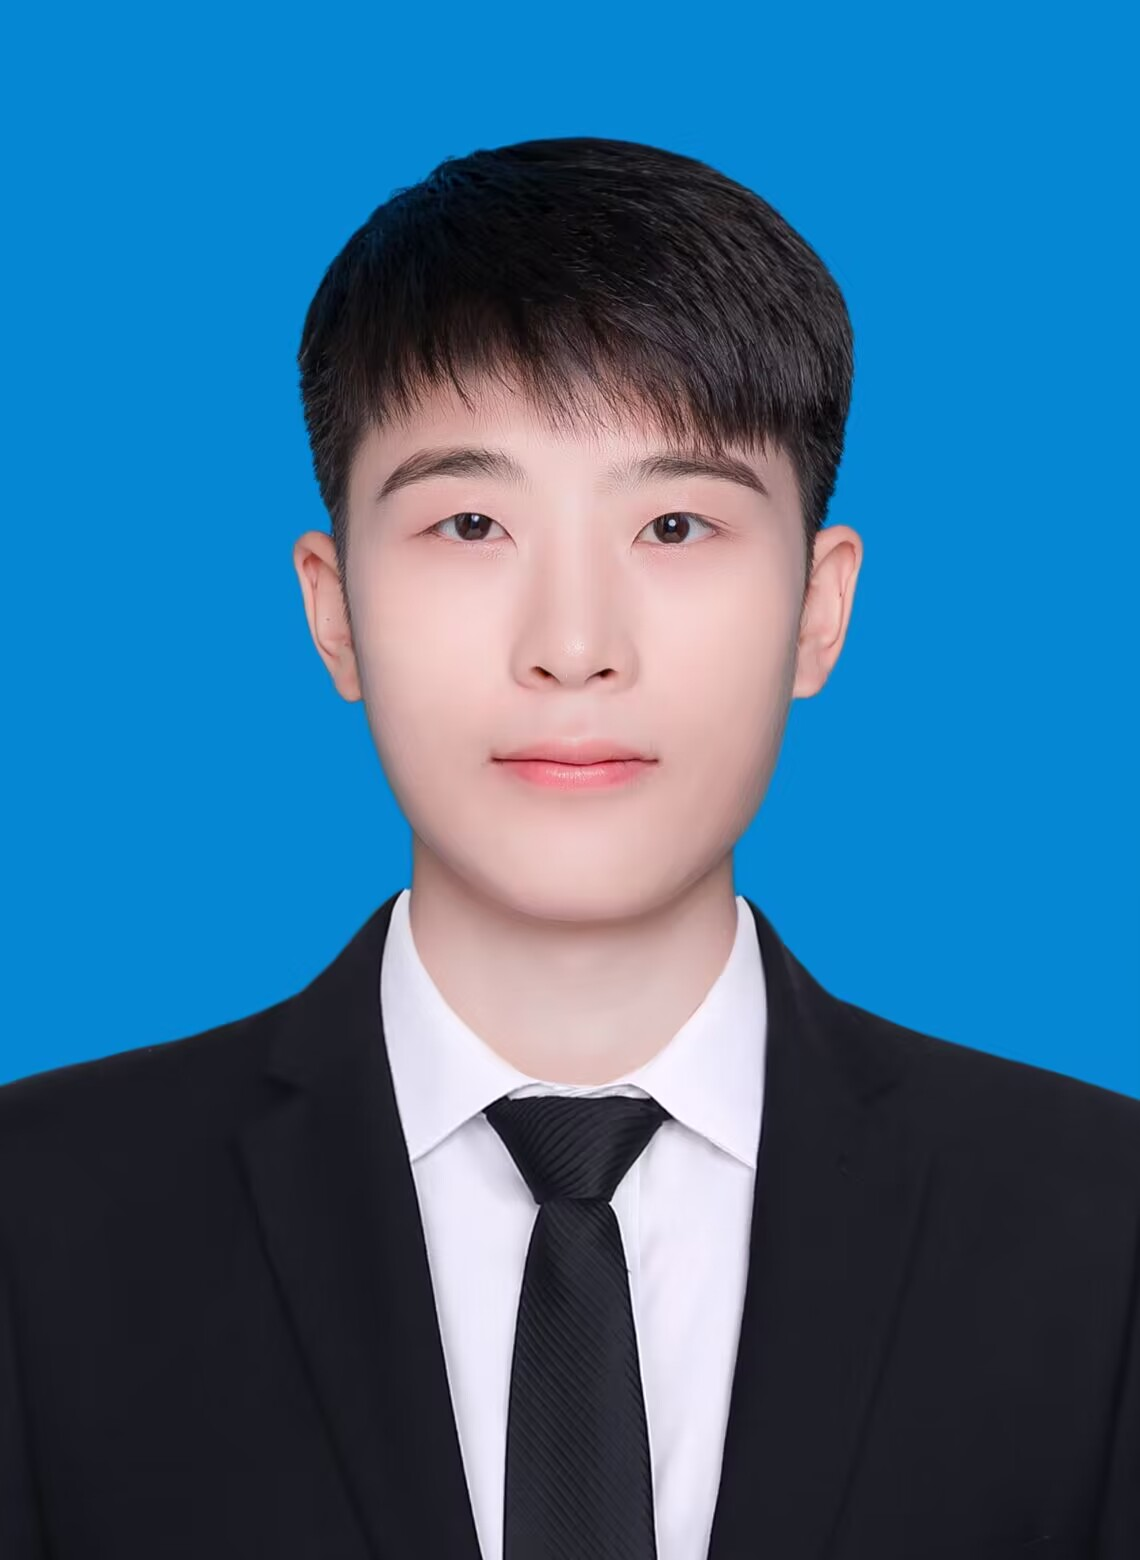
\includegraphics[width=1in,height=1.25in,clip,keepaspectratio]{picture/lhy.jpg}}] 
% {\bf Haoyu Lu} received the bachelor's degree from Zhengzhou University, China. He is currently working toward master's degree with the School of Computer Science and Technology, Huazhong University of Science and Technology, Wuhan, China. His research interests include dynamic graph and high performance computing.
% \end{IEEEbiography}
% \vspace{-1.5cm}

% \begin{IEEEbiography}
% [{\includegraphics[width=1in,height=1.25in,clip,keepaspectratio]{picture/yue.jpg}}] 
% {\bf Jianhui Yue} (Member, IEEE) received the PhD degree in computer science from the University of Maine, Orono, in 2012. He is an assistant professor of Computer Science Department, Michigan Technological University, Michigan. Before joining Michigan Technological University, he was a visiting assistant professor with Miami University, Ohio. His research interests include computer architecture, systems, and accelerator designs for machine learning. He received the Best Paper Award at IEEE CLUSTER 2007 and was the Best Paper Award candidate at HPCA 2013.
% \end{IEEEbiography}
% \vspace{-1.3cm}

% \begin{IEEEbiography}
% [{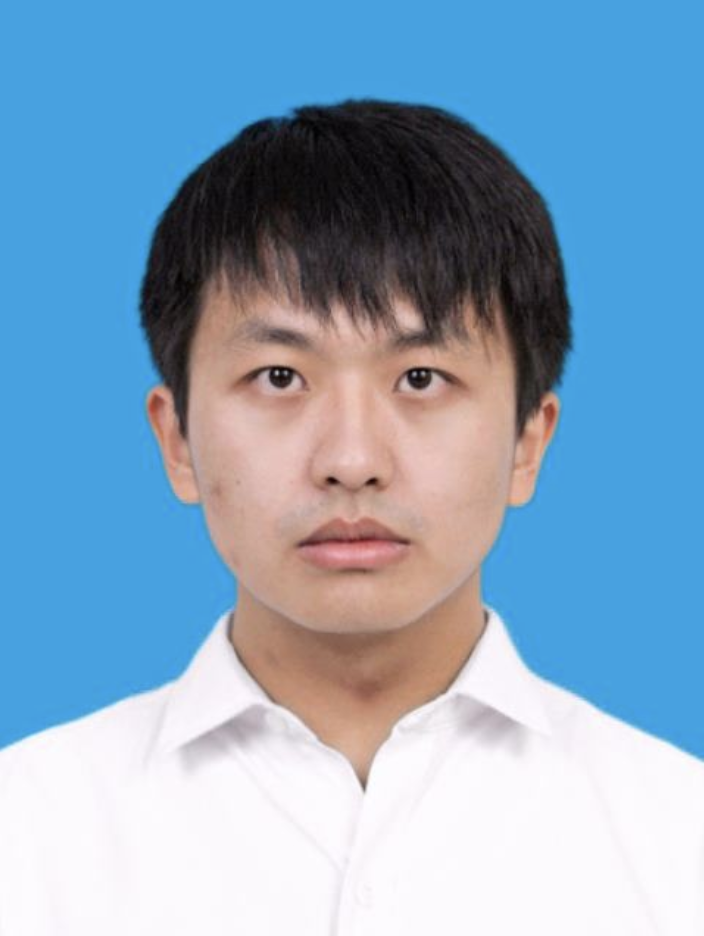
\includegraphics[width=1in,height=1.25in,clip,keepaspectratio]{picture/lk.png}}] 
% {\bf Kang Luo} received the bachelor's degree from the School of Computer Science and Engineering, Northeastern University, China. He is currently working toward the master's degree with the School of Computer Science and Technology, Huazhong University of Science and Technology, China. His research interests include graph process and graph mining.
% \end{IEEEbiography}
% \vspace{-1.3cm}

% \begin{IEEEbiography}
% [{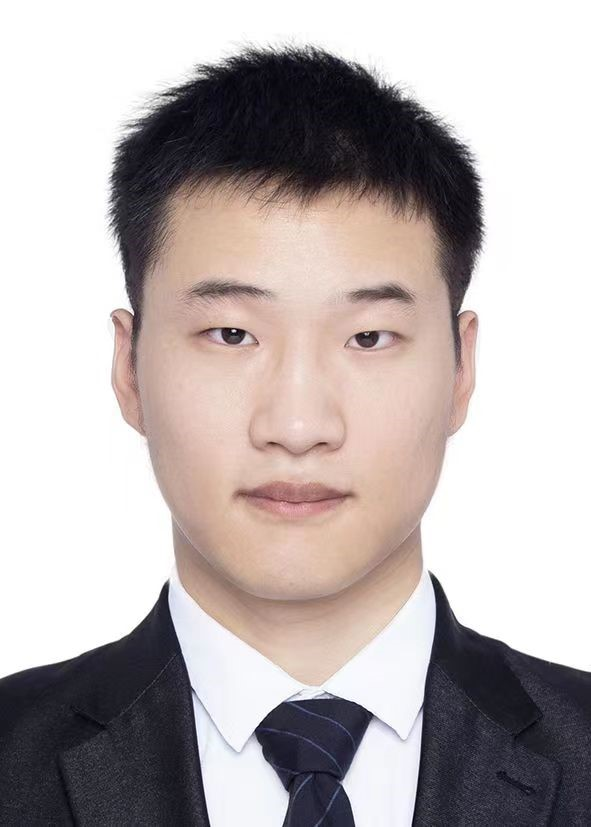
\includegraphics[width=1in,height=1.25in,clip,keepaspectratio]{picture/ywh.jpg}}] 
% {\bf Weihang Yin} received the bachelor's degree from Wuhan University, China. He is currently working toward master's degree with the School of Computer Science and Technology, Huazhong University of Science and Technology, Wuhan, China. His research interests include dynamic graph and large model.
% \end{IEEEbiography}
% \vspace{-1.3cm}

% \begin{IEEEbiography}
% [{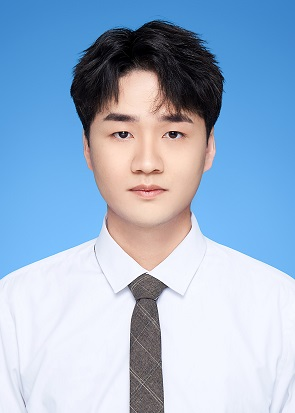
\includegraphics[width=1in,height=1.25in,clip,keepaspectratio]{picture/fyt.jpg}}] 
% {\bf Yutao Fu} received the bachelor's degree in software engineering from China University of Geosciences, Wuhan, China, in 2023. He is currently working toward the PhD degree with the school of computer science, Huazhong University of Science and Technology. His research interests include graph processing, system software, and architecture.
% \end{IEEEbiography}
% \vspace{-1.3cm}


% \begin{IEEEbiography}
% [{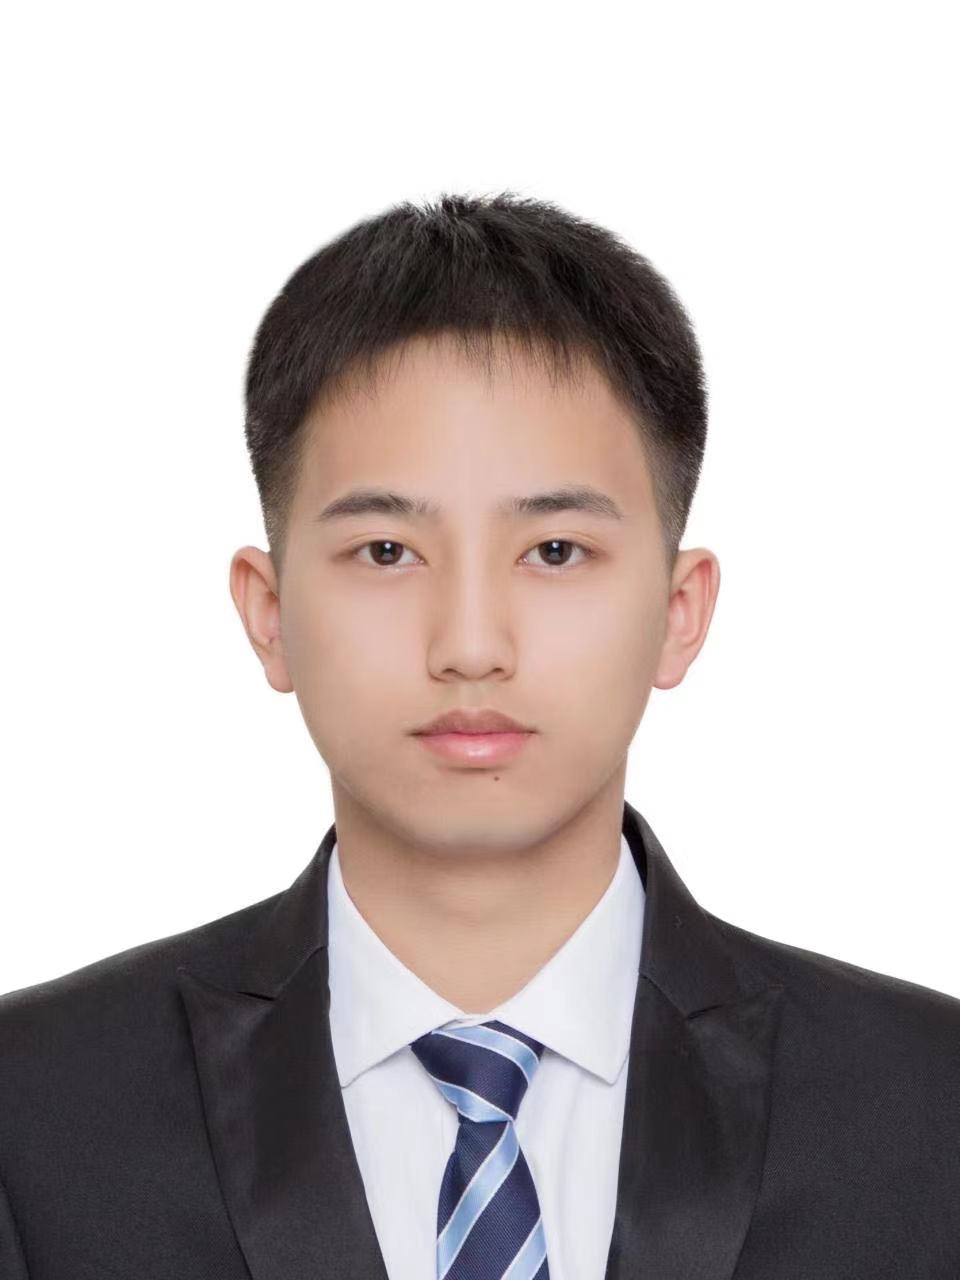
\includegraphics[width=1in,height=1.25in,clip,keepaspectratio]{picture/hzr.jpg}}] 
% {\bf Zirui He} received the bachelor's degree from the School of Software, Shandong University, Jinan, China. He is currently working toward the master's degree with the School of Computer and Science, Huazhong University of Science and Technology, China. His research interests include graph processing and graph neural networks.
% \end{IEEEbiography}
% \vspace{-1.3cm}

% \begin{IEEEbiography}
% [{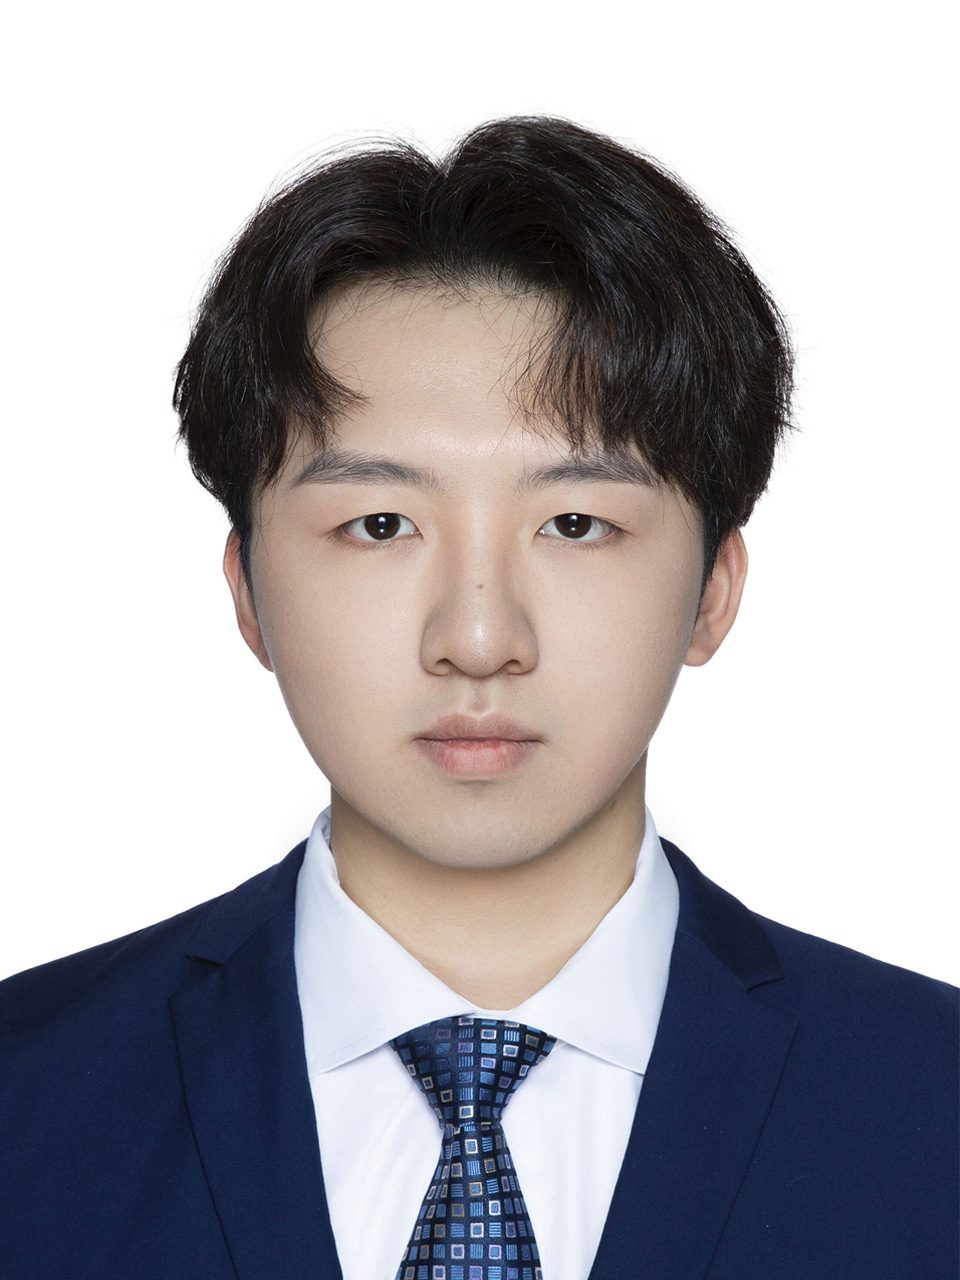
\includegraphics[width=1in,height=1.25in,clip,keepaspectratio]{picture/xxx.jpg}}] 
% {\bf Xiaoxuan Xu} received the bachelor's degree from the School of Intelligence Science and Technology, University of Science and Technology Beijing, China. He is currently working toward the master's degree with the School of Computer and Science, Huazhong University of Science and Technology, Wuhan, China. His research interests include dynamic graph and graph neural networks.
% \end{IEEEbiography}
% \vspace{-1.3cm}

% \begin{IEEEbiography}
% [{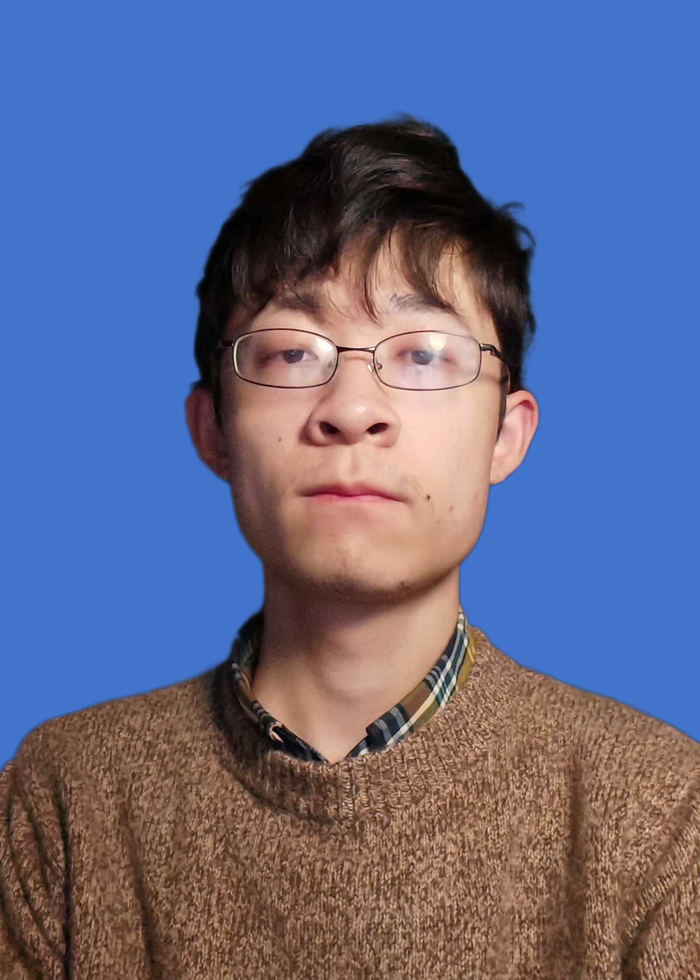
\includegraphics[width=1in,height=1.25in,clip,keepaspectratio]{picture/ljp.jpg}}] 
% {\bf Jiapeng Li} is an undergraudate from the School of Computer Science, Huazhong University of Science and Technology at Wuhan, China. His research interests include Graph Processing and Big Data Analysis.
% \end{IEEEbiography}
% \vspace{-0.8cm}

% \begin{IEEEbiography}
% [{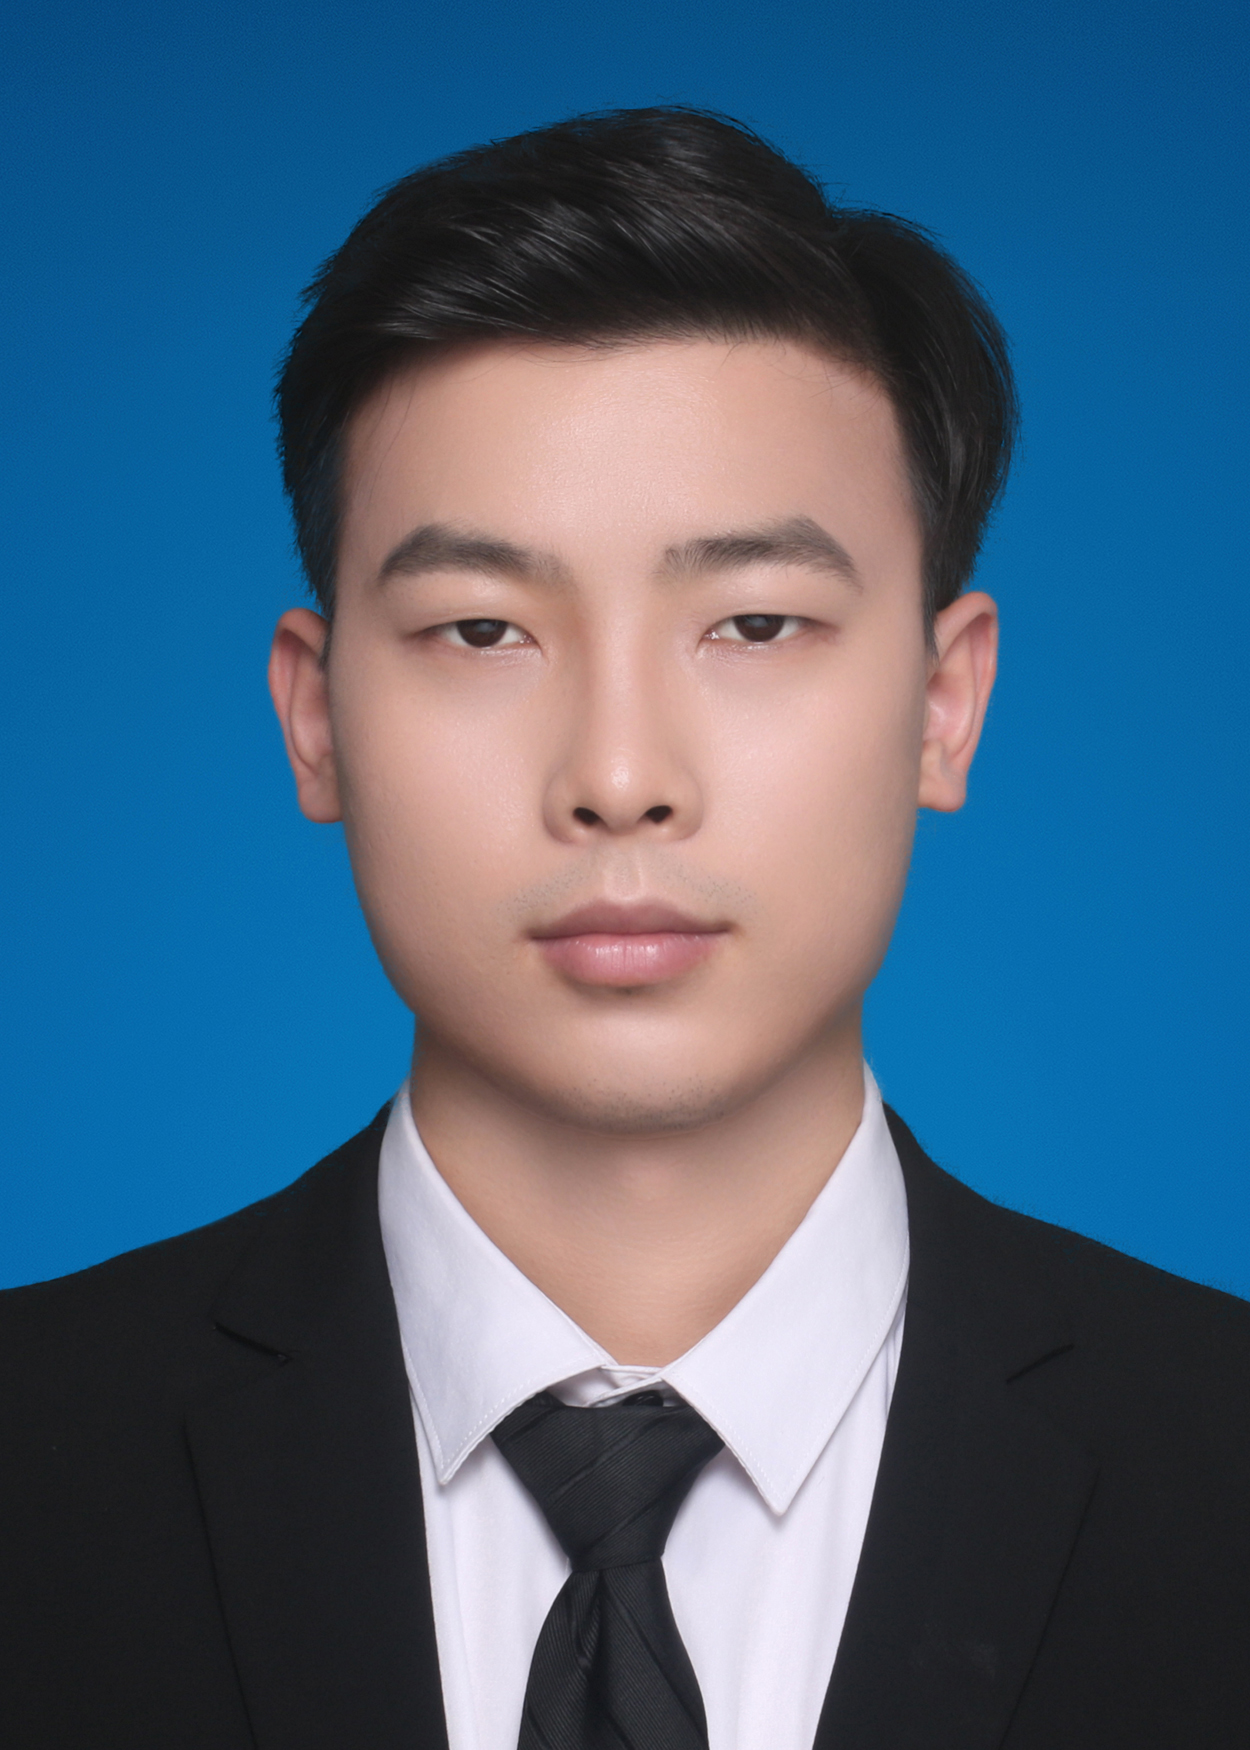
\includegraphics[width=1in,height=1.25in,clip,keepaspectratio]{picture/zjin.jpg}}] 
% {\bf Jin Zhao} received the PhD degree from the Huazhong University of Science and Technology, in 2022. He is now working toward the postdoctoral fellow at Zhejiang Lab, in China. His current research interests include graph processing, system software and architecture.
% \end{IEEEbiography}
% \vspace{-0.8cm}

% \begin{IEEEbiography}
% [{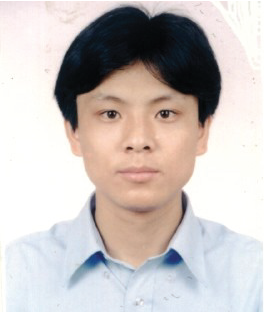
\includegraphics[width=1in,height=1.25in,clip,keepaspectratio]{picture/Xiaofei-eps-converted-to.png}}] 
% {\bf Xiaofei Liao} (Member, IEEE) received a PhD degree in computer science and engineering from Huazhong University of Science and Technology, China, in 2005. He is now a professor in school of Computer Science and Engineering at Huazhong University of Science and Technology. His research interests are in the areas of system virtualization, system software, and Cloud computing.
% \end{IEEEbiography}
% \vspace{-0.8cm}

% \begin{IEEEbiography}
% [{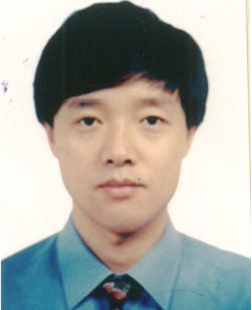
\includegraphics[width=1in,height=1.25in,clip,keepaspectratio]{picture/Hai-eps-converted-to.png}}]
% {\bf Hai Jin} (Fellow, IEEE) is a Cheung Kung Scholars Chair Professor of computer science and engineering at Huazhong University of Science and Technology in China. Jin received his PhD in computer engineering from Huazhong University of Science and Technology in 1994. In 1996, he was awarded a German Academic Exchange Service fellowship to visit the Technical University of Chemnitz in Germany. Jin worked at The University of Hong Kong between 1998 and 2000, and as a visiting scholar at the University of Southern California between 1999 and 2000. He was awarded Excellent Youth Award from the National Science Foundation of China in 2001. Jin is the chief scientist of ChinaGrid, the largest grid computing project in China, and the chief scientists of National 973 Basic Research Program Project of Virtualization Technology of Computing System, and Cloud Security. Jin is a Fellow of CCF, a Fellow of the IEEE and a member of the ACM. He has co-authored 22 books and published over 800 research papers. His research interests include computer architecture, virtualization technology, cluster computing and cloud computing, peer-to-peer computing, network storage, and network security.
% \end{IEEEbiography}
% \vfill



% if you will not have a photo at all

% You can push biographies down or up by placing
% a \vfill before or after them. The appropriate
% use of \vfill depends on what kind of text is
% on the last page and whether or not the columns
% are being equalized.

%\vfill

% Can be used to pull up biographies so that the bottom of the last one
% is flush with the other column.
%\enlargethispage{-5in}



% that's all folks
\end{document}


